% Generated by Sphinx.
\def\sphinxdocclass{report}
\documentclass[a4paper,10pt,english]{sphinxmanual}
\usepackage[utf8]{inputenc}
\DeclareUnicodeCharacter{00A0}{\nobreakspace}
\usepackage{cmap}
\usepackage[T1]{fontenc}
\usepackage{babel}
\usepackage{times}
\usepackage[Bjarne]{fncychap}
\usepackage{longtable}
\usepackage{sphinx}
\usepackage{multirow}

\addto\captionsenglish{\renewcommand{\figurename}{Fig. }}
\addto\captionsenglish{\renewcommand{\tablename}{Table }}
\floatname{literal-block}{Listing }



\title{pynoddy Documentation}
\date{October 11, 2015}
\release{}
\author{Florian Wellmann, Sam Thiele}
\newcommand{\sphinxlogo}{
\includegraphics{pynoddy_logo_3.pdf}\par}
\renewcommand{\releasename}{Release}
\makeindex

\makeatletter
\def\PYG@reset{\let\PYG@it=\relax \let\PYG@bf=\relax%
    \let\PYG@ul=\relax \let\PYG@tc=\relax%
    \let\PYG@bc=\relax \let\PYG@ff=\relax}
\def\PYG@tok#1{\csname PYG@tok@#1\endcsname}
\def\PYG@toks#1+{\ifx\relax#1\empty\else%
    \PYG@tok{#1}\expandafter\PYG@toks\fi}
\def\PYG@do#1{\PYG@bc{\PYG@tc{\PYG@ul{%
    \PYG@it{\PYG@bf{\PYG@ff{#1}}}}}}}
\def\PYG#1#2{\PYG@reset\PYG@toks#1+\relax+\PYG@do{#2}}

\expandafter\def\csname PYG@tok@gd\endcsname{\def\PYG@tc##1{\textcolor[rgb]{0.63,0.00,0.00}{##1}}}
\expandafter\def\csname PYG@tok@gu\endcsname{\let\PYG@bf=\textbf\def\PYG@tc##1{\textcolor[rgb]{0.50,0.00,0.50}{##1}}}
\expandafter\def\csname PYG@tok@gt\endcsname{\def\PYG@tc##1{\textcolor[rgb]{0.00,0.27,0.87}{##1}}}
\expandafter\def\csname PYG@tok@gs\endcsname{\let\PYG@bf=\textbf}
\expandafter\def\csname PYG@tok@gr\endcsname{\def\PYG@tc##1{\textcolor[rgb]{1.00,0.00,0.00}{##1}}}
\expandafter\def\csname PYG@tok@cm\endcsname{\let\PYG@it=\textit\def\PYG@tc##1{\textcolor[rgb]{0.25,0.50,0.56}{##1}}}
\expandafter\def\csname PYG@tok@vg\endcsname{\def\PYG@tc##1{\textcolor[rgb]{0.73,0.38,0.84}{##1}}}
\expandafter\def\csname PYG@tok@m\endcsname{\def\PYG@tc##1{\textcolor[rgb]{0.13,0.50,0.31}{##1}}}
\expandafter\def\csname PYG@tok@mh\endcsname{\def\PYG@tc##1{\textcolor[rgb]{0.13,0.50,0.31}{##1}}}
\expandafter\def\csname PYG@tok@cs\endcsname{\def\PYG@tc##1{\textcolor[rgb]{0.25,0.50,0.56}{##1}}\def\PYG@bc##1{\setlength{\fboxsep}{0pt}\colorbox[rgb]{1.00,0.94,0.94}{\strut ##1}}}
\expandafter\def\csname PYG@tok@ge\endcsname{\let\PYG@it=\textit}
\expandafter\def\csname PYG@tok@vc\endcsname{\def\PYG@tc##1{\textcolor[rgb]{0.73,0.38,0.84}{##1}}}
\expandafter\def\csname PYG@tok@il\endcsname{\def\PYG@tc##1{\textcolor[rgb]{0.13,0.50,0.31}{##1}}}
\expandafter\def\csname PYG@tok@go\endcsname{\def\PYG@tc##1{\textcolor[rgb]{0.20,0.20,0.20}{##1}}}
\expandafter\def\csname PYG@tok@cp\endcsname{\def\PYG@tc##1{\textcolor[rgb]{0.00,0.44,0.13}{##1}}}
\expandafter\def\csname PYG@tok@gi\endcsname{\def\PYG@tc##1{\textcolor[rgb]{0.00,0.63,0.00}{##1}}}
\expandafter\def\csname PYG@tok@gh\endcsname{\let\PYG@bf=\textbf\def\PYG@tc##1{\textcolor[rgb]{0.00,0.00,0.50}{##1}}}
\expandafter\def\csname PYG@tok@ni\endcsname{\let\PYG@bf=\textbf\def\PYG@tc##1{\textcolor[rgb]{0.84,0.33,0.22}{##1}}}
\expandafter\def\csname PYG@tok@nl\endcsname{\let\PYG@bf=\textbf\def\PYG@tc##1{\textcolor[rgb]{0.00,0.13,0.44}{##1}}}
\expandafter\def\csname PYG@tok@nn\endcsname{\let\PYG@bf=\textbf\def\PYG@tc##1{\textcolor[rgb]{0.05,0.52,0.71}{##1}}}
\expandafter\def\csname PYG@tok@no\endcsname{\def\PYG@tc##1{\textcolor[rgb]{0.38,0.68,0.84}{##1}}}
\expandafter\def\csname PYG@tok@na\endcsname{\def\PYG@tc##1{\textcolor[rgb]{0.25,0.44,0.63}{##1}}}
\expandafter\def\csname PYG@tok@nb\endcsname{\def\PYG@tc##1{\textcolor[rgb]{0.00,0.44,0.13}{##1}}}
\expandafter\def\csname PYG@tok@nc\endcsname{\let\PYG@bf=\textbf\def\PYG@tc##1{\textcolor[rgb]{0.05,0.52,0.71}{##1}}}
\expandafter\def\csname PYG@tok@nd\endcsname{\let\PYG@bf=\textbf\def\PYG@tc##1{\textcolor[rgb]{0.33,0.33,0.33}{##1}}}
\expandafter\def\csname PYG@tok@ne\endcsname{\def\PYG@tc##1{\textcolor[rgb]{0.00,0.44,0.13}{##1}}}
\expandafter\def\csname PYG@tok@nf\endcsname{\def\PYG@tc##1{\textcolor[rgb]{0.02,0.16,0.49}{##1}}}
\expandafter\def\csname PYG@tok@si\endcsname{\let\PYG@it=\textit\def\PYG@tc##1{\textcolor[rgb]{0.44,0.63,0.82}{##1}}}
\expandafter\def\csname PYG@tok@s2\endcsname{\def\PYG@tc##1{\textcolor[rgb]{0.25,0.44,0.63}{##1}}}
\expandafter\def\csname PYG@tok@vi\endcsname{\def\PYG@tc##1{\textcolor[rgb]{0.73,0.38,0.84}{##1}}}
\expandafter\def\csname PYG@tok@nt\endcsname{\let\PYG@bf=\textbf\def\PYG@tc##1{\textcolor[rgb]{0.02,0.16,0.45}{##1}}}
\expandafter\def\csname PYG@tok@nv\endcsname{\def\PYG@tc##1{\textcolor[rgb]{0.73,0.38,0.84}{##1}}}
\expandafter\def\csname PYG@tok@s1\endcsname{\def\PYG@tc##1{\textcolor[rgb]{0.25,0.44,0.63}{##1}}}
\expandafter\def\csname PYG@tok@gp\endcsname{\let\PYG@bf=\textbf\def\PYG@tc##1{\textcolor[rgb]{0.78,0.36,0.04}{##1}}}
\expandafter\def\csname PYG@tok@sh\endcsname{\def\PYG@tc##1{\textcolor[rgb]{0.25,0.44,0.63}{##1}}}
\expandafter\def\csname PYG@tok@ow\endcsname{\let\PYG@bf=\textbf\def\PYG@tc##1{\textcolor[rgb]{0.00,0.44,0.13}{##1}}}
\expandafter\def\csname PYG@tok@sx\endcsname{\def\PYG@tc##1{\textcolor[rgb]{0.78,0.36,0.04}{##1}}}
\expandafter\def\csname PYG@tok@bp\endcsname{\def\PYG@tc##1{\textcolor[rgb]{0.00,0.44,0.13}{##1}}}
\expandafter\def\csname PYG@tok@c1\endcsname{\let\PYG@it=\textit\def\PYG@tc##1{\textcolor[rgb]{0.25,0.50,0.56}{##1}}}
\expandafter\def\csname PYG@tok@kc\endcsname{\let\PYG@bf=\textbf\def\PYG@tc##1{\textcolor[rgb]{0.00,0.44,0.13}{##1}}}
\expandafter\def\csname PYG@tok@c\endcsname{\let\PYG@it=\textit\def\PYG@tc##1{\textcolor[rgb]{0.25,0.50,0.56}{##1}}}
\expandafter\def\csname PYG@tok@mf\endcsname{\def\PYG@tc##1{\textcolor[rgb]{0.13,0.50,0.31}{##1}}}
\expandafter\def\csname PYG@tok@err\endcsname{\def\PYG@bc##1{\setlength{\fboxsep}{0pt}\fcolorbox[rgb]{1.00,0.00,0.00}{1,1,1}{\strut ##1}}}
\expandafter\def\csname PYG@tok@mb\endcsname{\def\PYG@tc##1{\textcolor[rgb]{0.13,0.50,0.31}{##1}}}
\expandafter\def\csname PYG@tok@ss\endcsname{\def\PYG@tc##1{\textcolor[rgb]{0.32,0.47,0.09}{##1}}}
\expandafter\def\csname PYG@tok@sr\endcsname{\def\PYG@tc##1{\textcolor[rgb]{0.14,0.33,0.53}{##1}}}
\expandafter\def\csname PYG@tok@mo\endcsname{\def\PYG@tc##1{\textcolor[rgb]{0.13,0.50,0.31}{##1}}}
\expandafter\def\csname PYG@tok@kd\endcsname{\let\PYG@bf=\textbf\def\PYG@tc##1{\textcolor[rgb]{0.00,0.44,0.13}{##1}}}
\expandafter\def\csname PYG@tok@mi\endcsname{\def\PYG@tc##1{\textcolor[rgb]{0.13,0.50,0.31}{##1}}}
\expandafter\def\csname PYG@tok@kn\endcsname{\let\PYG@bf=\textbf\def\PYG@tc##1{\textcolor[rgb]{0.00,0.44,0.13}{##1}}}
\expandafter\def\csname PYG@tok@o\endcsname{\def\PYG@tc##1{\textcolor[rgb]{0.40,0.40,0.40}{##1}}}
\expandafter\def\csname PYG@tok@kr\endcsname{\let\PYG@bf=\textbf\def\PYG@tc##1{\textcolor[rgb]{0.00,0.44,0.13}{##1}}}
\expandafter\def\csname PYG@tok@s\endcsname{\def\PYG@tc##1{\textcolor[rgb]{0.25,0.44,0.63}{##1}}}
\expandafter\def\csname PYG@tok@kp\endcsname{\def\PYG@tc##1{\textcolor[rgb]{0.00,0.44,0.13}{##1}}}
\expandafter\def\csname PYG@tok@w\endcsname{\def\PYG@tc##1{\textcolor[rgb]{0.73,0.73,0.73}{##1}}}
\expandafter\def\csname PYG@tok@kt\endcsname{\def\PYG@tc##1{\textcolor[rgb]{0.56,0.13,0.00}{##1}}}
\expandafter\def\csname PYG@tok@sc\endcsname{\def\PYG@tc##1{\textcolor[rgb]{0.25,0.44,0.63}{##1}}}
\expandafter\def\csname PYG@tok@sb\endcsname{\def\PYG@tc##1{\textcolor[rgb]{0.25,0.44,0.63}{##1}}}
\expandafter\def\csname PYG@tok@k\endcsname{\let\PYG@bf=\textbf\def\PYG@tc##1{\textcolor[rgb]{0.00,0.44,0.13}{##1}}}
\expandafter\def\csname PYG@tok@se\endcsname{\let\PYG@bf=\textbf\def\PYG@tc##1{\textcolor[rgb]{0.25,0.44,0.63}{##1}}}
\expandafter\def\csname PYG@tok@sd\endcsname{\let\PYG@it=\textit\def\PYG@tc##1{\textcolor[rgb]{0.25,0.44,0.63}{##1}}}

\def\PYGZbs{\char`\\}
\def\PYGZus{\char`\_}
\def\PYGZob{\char`\{}
\def\PYGZcb{\char`\}}
\def\PYGZca{\char`\^}
\def\PYGZam{\char`\&}
\def\PYGZlt{\char`\<}
\def\PYGZgt{\char`\>}
\def\PYGZsh{\char`\#}
\def\PYGZpc{\char`\%}
\def\PYGZdl{\char`\$}
\def\PYGZhy{\char`\-}
\def\PYGZsq{\char`\'}
\def\PYGZdq{\char`\"}
\def\PYGZti{\char`\~}
% for compatibility with earlier versions
\def\PYGZat{@}
\def\PYGZlb{[}
\def\PYGZrb{]}
\makeatother

\renewcommand\PYGZsq{\textquotesingle}

\begin{document}

\maketitle
\tableofcontents
\phantomsection\label{index::doc}


Contents:


\chapter{pynoddy}
\label{readme:welcome-to-pynoddy-s-documentation}\label{readme::doc}\label{readme:pynoddy}
pynoddy is a python package to write, change, and analyse kinematic
geological modelling simulations performed with Noddy (see below for
more infomration on Noddy).


\section{How does it work?}
\label{readme:how-does-it-work}
At this stage, pynoddy provides wrapper modules for existing Noddy
history (.his) and result files (.g00, etc.). It is


\section{Installation}
\label{readme:installation}
To install pynoddy simply run:

\begin{Verbatim}[commandchars=\\\{\}]
python setup.py install
\end{Verbatim}

Note:
\begin{itemize}
\item {} 
sufficient privileges are required (i.e. run in sudo with MacOSX/
Linux and set permissions on Windows)

\end{itemize}

Important: the Noddy executable has to be in a directory defined in the
PATH variable!!

Important: the topology executable has to be in a directory defined in
the PATH variable!!


\section{Documentation}
\label{readme:documentation}

\section{Tutorial}
\label{readme:tutorial}
A tutorial starting with simple examples for changing the geological
history and visualisation of output, as well as the implementation of
stochastic simulations and uncertainty visualisation are available as
interactive ipython notebooks.


\section{Dependencies}
\label{readme:dependencies}
pynoddy depends on several standard Python packages that should be
shipped with any standard distribution (and are easy to install,
otherwise):

. numpy . matplotlib . pickle

The uncertainty anaysis, quantification, and visualisation methods based
on information theory are implemented in the python package pygeoinfo.
This package is available on github and part of the python package
index. It is automatically installed with the setup script provided with
this package. For more information, please see:

(todo: include package info!)

In addition, to export model results for full 3-D visualisation with
VTK, the pyevtk package is used, available on bitbucket:

\href{https://bitbucket.org/pauloh/pyevtk/src/9c19e3a54d1e?at=v0.1.0}{https://bitbucket.org/pauloh/pyevtk/src/9c19e3a54d1e?at=v0.1.0}

The package is automatically downloaded and installed when running
python setup.py install.


\section{License}
\label{readme:license}
pynoddy is free software and published under a MIT license (see license
file included in the repository). Please attribute the work when you use
it, feel free to change and adapt it otherwise!


\section{What is Noddy?}
\label{readme:what-is-noddy}
Noddy itself is a kinematic modelling program written by Mark Jessell
{[}1{]}{[}2{]} to simulate the effect of subsequent geological events (folding,
unconformities, faulting, etc.) on a primary sedimentary pile. A typical
example would be:
\begin{enumerate}
\item {} 
Create a sedimentary pile with defined thicknesses for multiple
formations

\item {} 
Add a folding event (for example simple sinoidal folding, but complex
methods are possible!)

\item {} 
Add an unconformity and, above it, a new stratigraphy

\item {} 
Finally, add a sequence of late faults affecting the entire system.

\end{enumerate}

The result could look something like this:

The software runs on Windows only, but the source files (written in C)
are available for download to generate a command line version of the
modelling step alone:

\href{https://github.com/flohorovicic/pynoddy}{https://github.com/flohorovicic/pynoddy}

It has been tested and compiled on MacOSX, Windows and Linux.


\section{References}
\label{readme:references}
{[}1{]} Mark W. Jessell. Noddy, an interactive map creation package.
Unpublished MSc Thesis, University of London. 1981. {[}2{]} Mark W. Jessell,
Rick K. Valenta, Structural geophysics: Integrated structural and
geophysical modelling, In: Declan G. De Paor, Editor(s), Computer
Methods in the Geosciences, Pergamon, 1996, Volume 15, Pages 303-324,
ISSN 1874-561X, ISBN 9780080424309,
\href{http://dx.doi.org/10.1016/S1874-561X(96)80027-7}{http://dx.doi.org/10.1016/S1874-561X(96)80027-7}.


\chapter{Simulation of a Noddy history and visualisation of output}
\label{notebooks/1-Simulation:simulation-of-a-noddy-history-and-visualisation-of-output}\label{notebooks/1-Simulation::doc}
This example shows how the module pynoddy.history can be used to compute
the model, and how simple visualisations can be generated with
pynoddy.output.

\begin{Verbatim}[commandchars=\\\{\}]
\PYG{k+kn}{from} \PYG{n+nn}{IPython.core.display} \PYG{k+kn}{import} \PYG{n}{HTML}
\PYG{n}{css\PYGZus{}file} \PYG{o}{=} \PYG{l+s}{\PYGZsq{}}\PYG{l+s}{pynoddy.css}\PYG{l+s}{\PYGZsq{}}
\PYG{n}{HTML}\PYG{p}{(}\PYG{n+nb}{open}\PYG{p}{(}\PYG{n}{css\PYGZus{}file}\PYG{p}{,} \PYG{l+s}{\PYGZdq{}}\PYG{l+s}{r}\PYG{l+s}{\PYGZdq{}}\PYG{p}{)}\PYG{o}{.}\PYG{n}{read}\PYG{p}{(}\PYG{p}{)}\PYG{p}{)}
\end{Verbatim}

\begin{Verbatim}[commandchars=\\\{\}]
\PYGZpc{}matplotlib inline
\end{Verbatim}

\begin{Verbatim}[commandchars=\\\{\}]
\PYG{c}{\PYGZsh{} Basic settings}
\PYG{k+kn}{import} \PYG{n+nn}{sys}\PYG{o}{,} \PYG{n+nn}{os}
\PYG{k+kn}{import} \PYG{n+nn}{subprocess}

\PYG{c}{\PYGZsh{} Now import pynoddy}
\PYG{k+kn}{import} \PYG{n+nn}{pynoddy}
\PYG{n+nb}{reload}\PYG{p}{(}\PYG{n}{pynoddy}\PYG{p}{)}
\PYG{k+kn}{import} \PYG{n+nn}{pynoddy.output}
\PYG{k+kn}{import} \PYG{n+nn}{pynoddy.history}

\PYG{c}{\PYGZsh{} determine path of repository to set paths corretly below}
\PYG{n}{repo\PYGZus{}path} \PYG{o}{=} \PYG{n}{os}\PYG{o}{.}\PYG{n}{path}\PYG{o}{.}\PYG{n}{realpath}\PYG{p}{(}\PYG{l+s}{\PYGZsq{}}\PYG{l+s}{../..}\PYG{l+s}{\PYGZsq{}}\PYG{p}{)}
\end{Verbatim}


\section{Compute the model}
\label{notebooks/1-Simulation:compute-the-model}
The simplest way to perform the Noddy simulation through Python is
simply to call the executable. One way that should be fairly platform
independent is to use Python's own subprocess module:

\begin{Verbatim}[commandchars=\\\{\}]
\PYG{c}{\PYGZsh{} Change to sandbox directory to store results}
\PYG{n}{os}\PYG{o}{.}\PYG{n}{chdir}\PYG{p}{(}\PYG{n}{os}\PYG{o}{.}\PYG{n}{path}\PYG{o}{.}\PYG{n}{join}\PYG{p}{(}\PYG{n}{repo\PYGZus{}path}\PYG{p}{,} \PYG{l+s}{\PYGZsq{}}\PYG{l+s}{sandbox}\PYG{l+s}{\PYGZsq{}}\PYG{p}{)}\PYG{p}{)}

\PYG{c}{\PYGZsh{} Path to exmaple directory in this repository}
\PYG{n}{example\PYGZus{}directory} \PYG{o}{=} \PYG{n}{os}\PYG{o}{.}\PYG{n}{path}\PYG{o}{.}\PYG{n}{join}\PYG{p}{(}\PYG{n}{repo\PYGZus{}path}\PYG{p}{,}\PYG{l+s}{\PYGZsq{}}\PYG{l+s}{examples}\PYG{l+s}{\PYGZsq{}}\PYG{p}{)}
\PYG{c}{\PYGZsh{} Compute noddy model for history file}
\PYG{n}{history\PYGZus{}file} \PYG{o}{=} \PYG{l+s}{\PYGZsq{}}\PYG{l+s}{simple\PYGZus{}two\PYGZus{}faults.his}\PYG{l+s}{\PYGZsq{}}
\PYG{n}{history} \PYG{o}{=} \PYG{n}{os}\PYG{o}{.}\PYG{n}{path}\PYG{o}{.}\PYG{n}{join}\PYG{p}{(}\PYG{n}{example\PYGZus{}directory}\PYG{p}{,} \PYG{n}{history\PYGZus{}file}\PYG{p}{)}
\PYG{n}{output\PYGZus{}name} \PYG{o}{=} \PYG{l+s}{\PYGZsq{}}\PYG{l+s}{noddy\PYGZus{}out}\PYG{l+s}{\PYGZsq{}}
\PYG{c}{\PYGZsh{} call Noddy}

\PYG{c}{\PYGZsh{} NOTE: Make sure that the noddy executable is accessible in the system!!}
\PYG{k}{print} \PYG{n}{subprocess}\PYG{o}{.}\PYG{n}{Popen}\PYG{p}{(}\PYG{p}{[}\PYG{l+s}{\PYGZsq{}}\PYG{l+s}{noddy.exe}\PYG{l+s}{\PYGZsq{}}\PYG{p}{,} \PYG{n}{history}\PYG{p}{,} \PYG{n}{output\PYGZus{}name}\PYG{p}{,} \PYG{l+s}{\PYGZsq{}}\PYG{l+s}{BLOCK}\PYG{l+s}{\PYGZsq{}}\PYG{p}{]}\PYG{p}{,}
                       \PYG{n}{shell}\PYG{o}{=}\PYG{n+nb+bp}{False}\PYG{p}{,} \PYG{n}{stderr}\PYG{o}{=}\PYG{n}{subprocess}\PYG{o}{.}\PYG{n}{PIPE}\PYG{p}{,}
                       \PYG{n}{stdout}\PYG{o}{=}\PYG{n}{subprocess}\PYG{o}{.}\PYG{n}{PIPE}\PYG{p}{)}\PYG{o}{.}\PYG{n}{stdout}\PYG{o}{.}\PYG{n}{read}\PYG{p}{(}\PYG{p}{)}
\PYG{c}{\PYGZsh{}}
\end{Verbatim}

For convenience, the model computation is wrapped into a Python function
in pynoddy:

\begin{Verbatim}[commandchars=\\\{\}]
\PYG{n}{pynoddy}\PYG{o}{.}\PYG{n}{compute\PYGZus{}model}\PYG{p}{(}\PYG{n}{history}\PYG{p}{,} \PYG{n}{output\PYGZus{}name}\PYG{p}{)}
\end{Verbatim}

\begin{Verbatim}[commandchars=\\\{\}]
\PYG{l+s}{\PYGZsq{}}\PYG{l+s}{\PYGZsq{}}
\end{Verbatim}

Note: The Noddy call from Python is, to date, calling Noddy through the
subprocess function. In a future implementation, this call could be
substituted with a full wrapper for the C-functions written in Python.
Therefore, using the member function compute\_model is not only easier,
but also the more ``future-proof'' way to compute the Noddy model.


\section{Loading Noddy output files}
\label{notebooks/1-Simulation:loading-noddy-output-files}
Noddy simulations produce a variety of different output files, depending
on the type of simulation. The basic output is the geological model.
Additional output files can contain geophysical responses, etc.

Loading the output files is simplified with a class class container that
reads all relevant information and provides simple methods for plotting,
model analysis, and export. To load the output information into a Python
object:

\begin{Verbatim}[commandchars=\\\{\}]
\PYG{n}{N1} \PYG{o}{=} \PYG{n}{pynoddy}\PYG{o}{.}\PYG{n}{output}\PYG{o}{.}\PYG{n}{NoddyOutput}\PYG{p}{(}\PYG{n}{output\PYGZus{}name}\PYG{p}{)}
\end{Verbatim}

The object contains the calculated geology blocks and some additional
information on grid spacing, model extent, etc. For example:

\begin{Verbatim}[commandchars=\\\{\}]
\PYG{k}{print}\PYG{p}{(}\PYG{l+s}{\PYGZdq{}}\PYG{l+s}{The model has an extent of }\PYG{l+s+si}{\PYGZpc{}.0f}\PYG{l+s}{ m in x\PYGZhy{}direction, with }\PYG{l+s+si}{\PYGZpc{}d}\PYG{l+s}{ cells of width }\PYG{l+s+si}{\PYGZpc{}.0f}\PYG{l+s}{ m}\PYG{l+s}{\PYGZdq{}} \PYG{o}{\PYGZpc{}}
      \PYG{p}{(}\PYG{n}{N1}\PYG{o}{.}\PYG{n}{extent\PYGZus{}x}\PYG{p}{,} \PYG{n}{N1}\PYG{o}{.}\PYG{n}{nx}\PYG{p}{,} \PYG{n}{N1}\PYG{o}{.}\PYG{n}{delx}\PYG{p}{)}\PYG{p}{)}
\end{Verbatim}

\begin{Verbatim}[commandchars=\\\{\}]
The model has an extent of 12400 m in x\PYGZhy{}direction, with 124 cells of width 100 m
\end{Verbatim}


\section{Plotting sections through the model}
\label{notebooks/1-Simulation:plotting-sections-through-the-model}
The NoddyOutput class has some basic methods for the visualisation of
the generated models. To plot sections through the model:

\begin{Verbatim}[commandchars=\\\{\}]
\PYG{n}{N1}\PYG{o}{.}\PYG{n}{plot\PYGZus{}section}\PYG{p}{(}\PYG{l+s}{\PYGZsq{}}\PYG{l+s}{y}\PYG{l+s}{\PYGZsq{}}\PYG{p}{,} \PYG{n}{figsize} \PYG{o}{=} \PYG{p}{(}\PYG{l+m+mi}{5}\PYG{p}{,}\PYG{l+m+mi}{3}\PYG{p}{)}\PYG{p}{)}
\end{Verbatim}
\begin{figure}[htbp]
\centering
\capstart

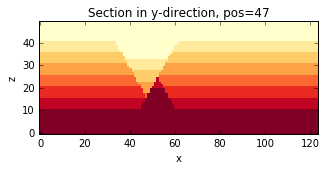
\includegraphics{1-Simulation_14_0.png}
\caption{png}\end{figure}


\section{Export model to VTK}
\label{notebooks/1-Simulation:export-model-to-vtk}
A simple possibility to visualise the modeled results in 3-D is to
export the model to a VTK file and then to visualise it with a VTK
viewer, for example Paraview. To export the model, simply use:

\begin{Verbatim}[commandchars=\\\{\}]
\PYG{n}{N1}\PYG{o}{.}\PYG{n}{export\PYGZus{}to\PYGZus{}vtk}\PYG{p}{(}\PYG{p}{)}
\end{Verbatim}

The exported VTK file can be visualised in any VTK viewer, for example
in the (free) viewer Paraview (www.paraview.org). An example
visualisation of the model in 3-D is presented in the figure below.
\begin{figure}[htbp]
\centering
\capstart

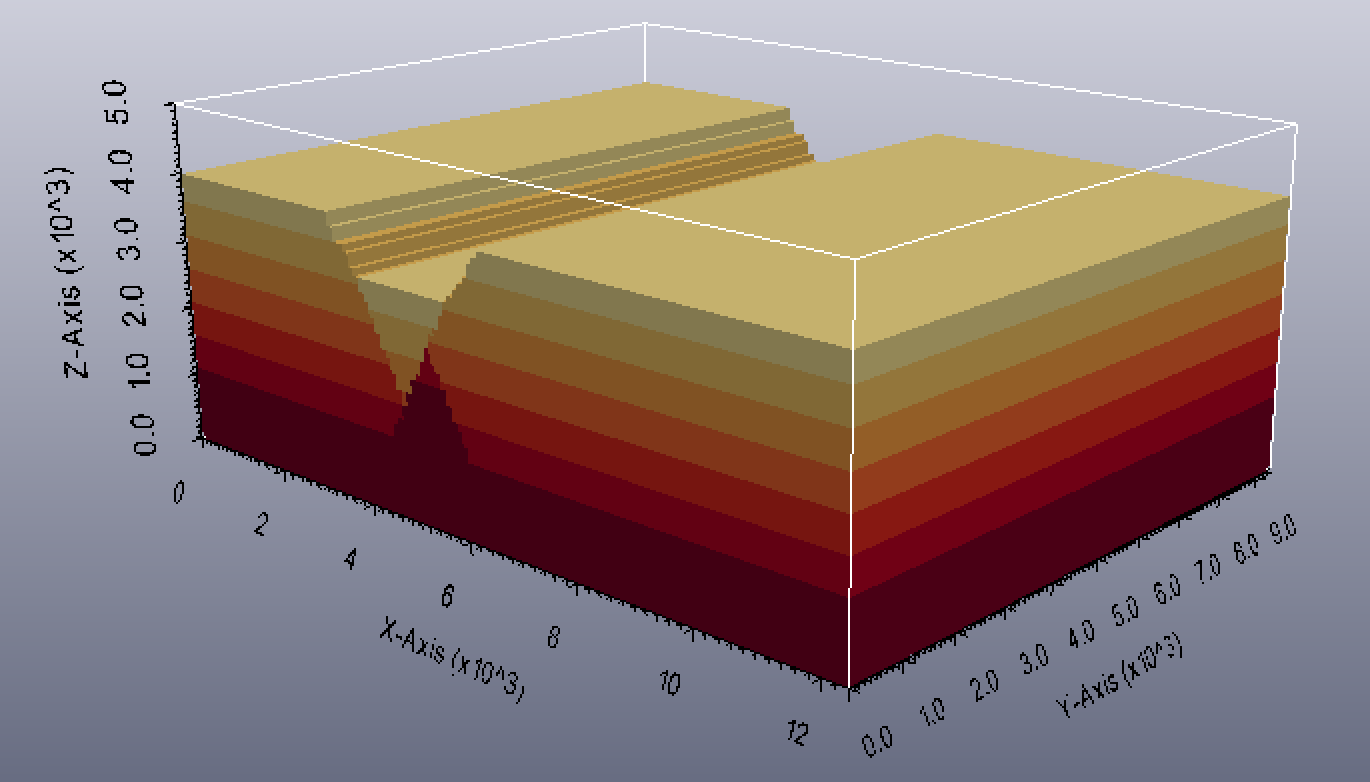
\includegraphics{3d_render_fault_model_2.png}
\caption{3-D Visualisation generated with Paraview (top layer transparent)}\end{figure}


\chapter{Change Noddy input file and recompute model}
\label{notebooks/2-Adjust-input::doc}\label{notebooks/2-Adjust-input:change-noddy-input-file-and-recompute-model}
In this section, we will briefly present possibilities to access the
properties defined in the Noddy history input file and show how simple
adjustments can be performed, for example changing the cube size to
obtain a model with a higher resolution.

Also outlined here is the way that events are stored in the history file
as single objects. For more information on accessing and changing the
events themselves, please be patient until we get to the next section.

\begin{Verbatim}[commandchars=\\\{\}]
\PYG{k+kn}{from} \PYG{n+nn}{IPython.core.display} \PYG{k+kn}{import} \PYG{n}{HTML}
\PYG{n}{css\PYGZus{}file} \PYG{o}{=} \PYG{l+s}{\PYGZsq{}}\PYG{l+s}{pynoddy.css}\PYG{l+s}{\PYGZsq{}}
\PYG{n}{HTML}\PYG{p}{(}\PYG{n+nb}{open}\PYG{p}{(}\PYG{n}{css\PYGZus{}file}\PYG{p}{,} \PYG{l+s}{\PYGZdq{}}\PYG{l+s}{r}\PYG{l+s}{\PYGZdq{}}\PYG{p}{)}\PYG{o}{.}\PYG{n}{read}\PYG{p}{(}\PYG{p}{)}\PYG{p}{)}
\end{Verbatim}

\begin{Verbatim}[commandchars=\\\{\}]
cd ../docs/notebooks/
\end{Verbatim}

\begin{Verbatim}[commandchars=\\\{\}]
/Users/flow/git/pynoddy/docs/notebooks
\end{Verbatim}

\begin{Verbatim}[commandchars=\\\{\}]
\PYGZpc{}matplotlib inline
\end{Verbatim}

\begin{Verbatim}[commandchars=\\\{\}]
\PYG{k+kn}{import} \PYG{n+nn}{sys}\PYG{o}{,} \PYG{n+nn}{os}
\PYG{k+kn}{import} \PYG{n+nn}{matplotlib.pyplot} \PYG{k+kn}{as} \PYG{n+nn}{plt}
\PYG{k+kn}{import} \PYG{n+nn}{numpy} \PYG{k+kn}{as} \PYG{n+nn}{np}
\PYG{c}{\PYGZsh{} adjust some settings for matplotlib}
\PYG{k+kn}{from} \PYG{n+nn}{matplotlib} \PYG{k+kn}{import} \PYG{n}{rcParams}
\PYG{c}{\PYGZsh{} print rcParams}
\PYG{n}{rcParams}\PYG{p}{[}\PYG{l+s}{\PYGZsq{}}\PYG{l+s}{font.size}\PYG{l+s}{\PYGZsq{}}\PYG{p}{]} \PYG{o}{=} \PYG{l+m+mi}{15}
\PYG{c}{\PYGZsh{} determine path of repository to set paths corretly below}
\PYG{n}{repo\PYGZus{}path} \PYG{o}{=} \PYG{n}{os}\PYG{o}{.}\PYG{n}{path}\PYG{o}{.}\PYG{n}{realpath}\PYG{p}{(}\PYG{l+s}{\PYGZsq{}}\PYG{l+s}{../..}\PYG{l+s}{\PYGZsq{}}\PYG{p}{)}
\PYG{k+kn}{import} \PYG{n+nn}{pynoddy}
\PYG{k+kn}{import} \PYG{n+nn}{pynoddy.history}
\PYG{k+kn}{import} \PYG{n+nn}{pynoddy.output}
\end{Verbatim}

First step: load the history file into a Python object:

\begin{Verbatim}[commandchars=\\\{\}]
\PYG{c}{\PYGZsh{} Change to sandbox directory to store results}
\PYG{n}{os}\PYG{o}{.}\PYG{n}{chdir}\PYG{p}{(}\PYG{n}{os}\PYG{o}{.}\PYG{n}{path}\PYG{o}{.}\PYG{n}{join}\PYG{p}{(}\PYG{n}{repo\PYGZus{}path}\PYG{p}{,} \PYG{l+s}{\PYGZsq{}}\PYG{l+s}{sandbox}\PYG{l+s}{\PYGZsq{}}\PYG{p}{)}\PYG{p}{)}
\PYG{c}{\PYGZsh{} Path to exmaple directory in this repository}
\PYG{n}{example\PYGZus{}directory} \PYG{o}{=} \PYG{n}{os}\PYG{o}{.}\PYG{n}{path}\PYG{o}{.}\PYG{n}{join}\PYG{p}{(}\PYG{n}{repo\PYGZus{}path}\PYG{p}{,}\PYG{l+s}{\PYGZsq{}}\PYG{l+s}{examples}\PYG{l+s}{\PYGZsq{}}\PYG{p}{)}
\PYG{c}{\PYGZsh{} Compute noddy model for history file}
\PYG{n}{history\PYGZus{}file} \PYG{o}{=} \PYG{l+s}{\PYGZsq{}}\PYG{l+s}{simple\PYGZus{}two\PYGZus{}faults.his}\PYG{l+s}{\PYGZsq{}}
\PYG{n}{history} \PYG{o}{=} \PYG{n}{os}\PYG{o}{.}\PYG{n}{path}\PYG{o}{.}\PYG{n}{join}\PYG{p}{(}\PYG{n}{example\PYGZus{}directory}\PYG{p}{,} \PYG{n}{history\PYGZus{}file}\PYG{p}{)}
\PYG{n}{output\PYGZus{}name} \PYG{o}{=} \PYG{l+s}{\PYGZsq{}}\PYG{l+s}{noddy\PYGZus{}out}\PYG{l+s}{\PYGZsq{}}
\PYG{n}{H1} \PYG{o}{=} \PYG{n}{pynoddy}\PYG{o}{.}\PYG{n}{history}\PYG{o}{.}\PYG{n}{NoddyHistory}\PYG{p}{(}\PYG{n}{history}\PYG{p}{)}
\end{Verbatim}

\textbf{Technical note}: the \code{NoddyHistory} class can be accessed on the
level of pynoddy (as it is imported in the \code{\_\_init\_\_.py} module) with
the shortcut:

\code{H1 = pynoddy.NoddyHistory(history)}

I am using the long version \code{pynoddy.history.NoddyHistory} here to
ensure that the correct package is loaded with the \code{reload()}
function. If you don't make changes to any of the pynoddy files, this is
not required. So for any practical cases, the shortcuts are absolutely
fine!


\section{Get basic information on the model}
\label{notebooks/2-Adjust-input:get-basic-information-on-the-model}
The history file contains the entire information on the Noddy model.
Some information can be accessed through the NoddyHistory object (and
more will be added soon!), for example the total number of events:

\begin{Verbatim}[commandchars=\\\{\}]
\PYG{k}{print}\PYG{p}{(}\PYG{l+s}{\PYGZdq{}}\PYG{l+s}{The history contains }\PYG{l+s+si}{\PYGZpc{}d}\PYG{l+s}{ events}\PYG{l+s}{\PYGZdq{}} \PYG{o}{\PYGZpc{}} \PYG{n}{H1}\PYG{o}{.}\PYG{n}{n\PYGZus{}events}\PYG{p}{)}
\end{Verbatim}

\begin{Verbatim}[commandchars=\\\{\}]
The history contains 3 events
\end{Verbatim}

Events are implemented as objects, the classes are defined in
\code{H1.events}. All events are accessible in a list on the level of the
history object:

\begin{Verbatim}[commandchars=\\\{\}]
\PYG{n}{H1}\PYG{o}{.}\PYG{n}{events}
\end{Verbatim}

\begin{Verbatim}[commandchars=\\\{\}]
\PYGZob{}1: \PYGZlt{}pynoddy.events.Stratigraphy at 0x103ac2a50\PYGZgt{},
 2: \PYGZlt{}pynoddy.events.Fault at 0x103ac2a90\PYGZgt{},
 3: \PYGZlt{}pynoddy.events.Fault at 0x103ac2ad0\PYGZgt{}\PYGZcb{}
\end{Verbatim}

The properties of an event are stored in the event objects themselves.
To date, only a subset of the properties (deemed as relevant for the
purpose of pynoddy so far) are parsed. The .his file contains a lot more
information! If access to this information is required, adjustments in
pynoddy.events have to be made.

For example, the properties of a fault object are:

\begin{Verbatim}[commandchars=\\\{\}]
\PYG{n}{H1}\PYG{o}{.}\PYG{n}{events}\PYG{p}{[}\PYG{l+m+mi}{2}\PYG{p}{]}\PYG{o}{.}\PYG{n}{properties}
\PYG{c}{\PYGZsh{} print H1.events[5].properties.keys()}
\end{Verbatim}

\begin{Verbatim}[commandchars=\\\{\}]
\PYG{p}{\PYGZob{}}\PYG{l+s}{\PYGZsq{}}\PYG{l+s}{Amplitude}\PYG{l+s}{\PYGZsq{}}\PYG{p}{:} \PYG{l+m+mf}{2000.0}\PYG{p}{,}
 \PYG{l+s}{\PYGZsq{}}\PYG{l+s}{Blue}\PYG{l+s}{\PYGZsq{}}\PYG{p}{:} \PYG{l+m+mf}{254.0}\PYG{p}{,}
 \PYG{l+s}{\PYGZsq{}}\PYG{l+s}{Color Name}\PYG{l+s}{\PYGZsq{}}\PYG{p}{:} \PYG{l+s}{\PYGZsq{}}\PYG{l+s}{Custom Colour 8}\PYG{l+s}{\PYGZsq{}}\PYG{p}{,}
 \PYG{l+s}{\PYGZsq{}}\PYG{l+s}{Cyl Index}\PYG{l+s}{\PYGZsq{}}\PYG{p}{:} \PYG{l+m+mf}{0.0}\PYG{p}{,}
 \PYG{l+s}{\PYGZsq{}}\PYG{l+s}{Dip}\PYG{l+s}{\PYGZsq{}}\PYG{p}{:} \PYG{l+m+mf}{60.0}\PYG{p}{,}
 \PYG{l+s}{\PYGZsq{}}\PYG{l+s}{Dip Direction}\PYG{l+s}{\PYGZsq{}}\PYG{p}{:} \PYG{l+m+mf}{90.0}\PYG{p}{,}
 \PYG{l+s}{\PYGZsq{}}\PYG{l+s}{Geometry}\PYG{l+s}{\PYGZsq{}}\PYG{p}{:} \PYG{l+s}{\PYGZsq{}}\PYG{l+s}{Translation}\PYG{l+s}{\PYGZsq{}}\PYG{p}{,}
 \PYG{l+s}{\PYGZsq{}}\PYG{l+s}{Green}\PYG{l+s}{\PYGZsq{}}\PYG{p}{:} \PYG{l+m+mf}{0.0}\PYG{p}{,}
 \PYG{l+s}{\PYGZsq{}}\PYG{l+s}{Movement}\PYG{l+s}{\PYGZsq{}}\PYG{p}{:} \PYG{l+s}{\PYGZsq{}}\PYG{l+s}{Hanging Wall}\PYG{l+s}{\PYGZsq{}}\PYG{p}{,}
 \PYG{l+s}{\PYGZsq{}}\PYG{l+s}{Pitch}\PYG{l+s}{\PYGZsq{}}\PYG{p}{:} \PYG{l+m+mf}{90.0}\PYG{p}{,}
 \PYG{l+s}{\PYGZsq{}}\PYG{l+s}{Profile Pitch}\PYG{l+s}{\PYGZsq{}}\PYG{p}{:} \PYG{l+m+mf}{90.0}\PYG{p}{,}
 \PYG{l+s}{\PYGZsq{}}\PYG{l+s}{Radius}\PYG{l+s}{\PYGZsq{}}\PYG{p}{:} \PYG{l+m+mf}{1000.0}\PYG{p}{,}
 \PYG{l+s}{\PYGZsq{}}\PYG{l+s}{Red}\PYG{l+s}{\PYGZsq{}}\PYG{p}{:} \PYG{l+m+mf}{0.0}\PYG{p}{,}
 \PYG{l+s}{\PYGZsq{}}\PYG{l+s}{Rotation}\PYG{l+s}{\PYGZsq{}}\PYG{p}{:} \PYG{l+m+mf}{30.0}\PYG{p}{,}
 \PYG{l+s}{\PYGZsq{}}\PYG{l+s}{Slip}\PYG{l+s}{\PYGZsq{}}\PYG{p}{:} \PYG{l+m+mf}{1000.0}\PYG{p}{,}
 \PYG{l+s}{\PYGZsq{}}\PYG{l+s}{X}\PYG{l+s}{\PYGZsq{}}\PYG{p}{:} \PYG{l+m+mf}{5500.0}\PYG{p}{,}
 \PYG{l+s}{\PYGZsq{}}\PYG{l+s}{XAxis}\PYG{l+s}{\PYGZsq{}}\PYG{p}{:} \PYG{l+m+mf}{2000.0}\PYG{p}{,}
 \PYG{l+s}{\PYGZsq{}}\PYG{l+s}{Y}\PYG{l+s}{\PYGZsq{}}\PYG{p}{:} \PYG{l+m+mf}{3968.0}\PYG{p}{,}
 \PYG{l+s}{\PYGZsq{}}\PYG{l+s}{YAxis}\PYG{l+s}{\PYGZsq{}}\PYG{p}{:} \PYG{l+m+mf}{2000.0}\PYG{p}{,}
 \PYG{l+s}{\PYGZsq{}}\PYG{l+s}{Z}\PYG{l+s}{\PYGZsq{}}\PYG{p}{:} \PYG{l+m+mf}{0.0}\PYG{p}{,}
 \PYG{l+s}{\PYGZsq{}}\PYG{l+s}{ZAxis}\PYG{l+s}{\PYGZsq{}}\PYG{p}{:} \PYG{l+m+mf}{2000.0}\PYG{p}{\PYGZcb{}}
\end{Verbatim}


\section{Change model cube size and recompute model}
\label{notebooks/2-Adjust-input:change-model-cube-size-and-recompute-model}
The Noddy model itself is, once computed, a continuous model in 3-D
space. However, for most visualisations and further calculations (e.g.
geophysics), a discretised version is suitable. The discretisation (or
block size) can be adapted in the history file. The according pynoddy
function is change\_cube\_size.

A simple example to change the cube size and write a new history file:

\begin{Verbatim}[commandchars=\\\{\}]
\PYG{c}{\PYGZsh{} We will first recompute the model and store results in an output file for comparison}
\PYG{n}{NH1} \PYG{o}{=} \PYG{n}{pynoddy}\PYG{o}{.}\PYG{n}{history}\PYG{o}{.}\PYG{n}{NoddyHistory}\PYG{p}{(}\PYG{n}{history}\PYG{p}{)}
\PYG{n}{pynoddy}\PYG{o}{.}\PYG{n}{compute\PYGZus{}model}\PYG{p}{(}\PYG{n}{history}\PYG{p}{,} \PYG{n}{output\PYGZus{}name}\PYG{p}{)}
\PYG{n}{NO1} \PYG{o}{=} \PYG{n}{pynoddy}\PYG{o}{.}\PYG{n}{output}\PYG{o}{.}\PYG{n}{NoddyOutput}\PYG{p}{(}\PYG{n}{output\PYGZus{}name}\PYG{p}{)}
\end{Verbatim}

\begin{Verbatim}[commandchars=\\\{\}]
\PYG{c}{\PYGZsh{} Now: change cubsize, write to new file and recompute}
\PYG{n}{NH1}\PYG{o}{.}\PYG{n}{change\PYGZus{}cube\PYGZus{}size}\PYG{p}{(}\PYG{l+m+mi}{50}\PYG{p}{)}
\PYG{c}{\PYGZsh{} Save model to a new history file and recompute (Note: may take a while to compute now)}
\PYG{n}{new\PYGZus{}history} \PYG{o}{=} \PYG{l+s}{\PYGZdq{}}\PYG{l+s}{fault\PYGZus{}model\PYGZus{}changed\PYGZus{}cubesize.his}\PYG{l+s}{\PYGZdq{}}
\PYG{n}{new\PYGZus{}output\PYGZus{}name} \PYG{o}{=} \PYG{l+s}{\PYGZdq{}}\PYG{l+s}{noddy\PYGZus{}out\PYGZus{}changed\PYGZus{}cube}\PYG{l+s}{\PYGZdq{}}
\PYG{n}{NH1}\PYG{o}{.}\PYG{n}{write\PYGZus{}history}\PYG{p}{(}\PYG{n}{new\PYGZus{}history}\PYG{p}{)}
\PYG{n}{pynoddy}\PYG{o}{.}\PYG{n}{compute\PYGZus{}model}\PYG{p}{(}\PYG{n}{new\PYGZus{}history}\PYG{p}{,} \PYG{n}{new\PYGZus{}output\PYGZus{}name}\PYG{p}{)}
\PYG{n}{NO2} \PYG{o}{=} \PYG{n}{pynoddy}\PYG{o}{.}\PYG{n}{output}\PYG{o}{.}\PYG{n}{NoddyOutput}\PYG{p}{(}\PYG{n}{new\PYGZus{}output\PYGZus{}name}\PYG{p}{)}
\end{Verbatim}

The different cell sizes are also represented in the output files:

\begin{Verbatim}[commandchars=\\\{\}]
\PYG{k}{print}\PYG{p}{(}\PYG{l+s}{\PYGZdq{}}\PYG{l+s}{Model 1 contains a total of }\PYG{l+s+si}{\PYGZpc{}7d}\PYG{l+s}{ cells with a blocksize }\PYG{l+s+si}{\PYGZpc{}.0f}\PYG{l+s}{ m}\PYG{l+s}{\PYGZdq{}} \PYG{o}{\PYGZpc{}}
      \PYG{p}{(}\PYG{n}{NO1}\PYG{o}{.}\PYG{n}{n\PYGZus{}total}\PYG{p}{,} \PYG{n}{NO1}\PYG{o}{.}\PYG{n}{delx}\PYG{p}{)}\PYG{p}{)}
\PYG{k}{print}\PYG{p}{(}\PYG{l+s}{\PYGZdq{}}\PYG{l+s}{Model 2 contains a total of }\PYG{l+s+si}{\PYGZpc{}7d}\PYG{l+s}{ cells with a blocksize }\PYG{l+s+si}{\PYGZpc{}.0f}\PYG{l+s}{ m}\PYG{l+s}{\PYGZdq{}} \PYG{o}{\PYGZpc{}}
      \PYG{p}{(}\PYG{n}{NO2}\PYG{o}{.}\PYG{n}{n\PYGZus{}total}\PYG{p}{,} \PYG{n}{NO2}\PYG{o}{.}\PYG{n}{delx}\PYG{p}{)}\PYG{p}{)}
\end{Verbatim}

\begin{Verbatim}[commandchars=\\\{\}]
Model 1 contains a total of  582800 cells with a blocksize 100 m
Model 2 contains a total of 4662400 cells with a blocksize 50 m
\end{Verbatim}

We can compare the effect of the different model discretisations in
section plots, created with the plot\_section method described before.
Let's get a bit more fancy here and use the functionality to pass axes
to the plot\_section method, and to create one figure as direct
comparison:

\begin{Verbatim}[commandchars=\\\{\}]
\PYG{c}{\PYGZsh{} create basic figure layout}
\PYG{n}{fig} \PYG{o}{=} \PYG{n}{plt}\PYG{o}{.}\PYG{n}{figure}\PYG{p}{(}\PYG{n}{figsize} \PYG{o}{=} \PYG{p}{(}\PYG{l+m+mi}{15}\PYG{p}{,}\PYG{l+m+mi}{5}\PYG{p}{)}\PYG{p}{)}
\PYG{n}{ax1} \PYG{o}{=} \PYG{n}{fig}\PYG{o}{.}\PYG{n}{add\PYGZus{}subplot}\PYG{p}{(}\PYG{l+m+mi}{121}\PYG{p}{)}
\PYG{n}{ax2} \PYG{o}{=} \PYG{n}{fig}\PYG{o}{.}\PYG{n}{add\PYGZus{}subplot}\PYG{p}{(}\PYG{l+m+mi}{122}\PYG{p}{)}
\PYG{n}{NO1}\PYG{o}{.}\PYG{n}{plot\PYGZus{}section}\PYG{p}{(}\PYG{l+s}{\PYGZsq{}}\PYG{l+s}{y}\PYG{l+s}{\PYGZsq{}}\PYG{p}{,} \PYG{n}{position}\PYG{o}{=}\PYG{l+m+mi}{0}\PYG{p}{,} \PYG{n}{ax} \PYG{o}{=} \PYG{n}{ax1}\PYG{p}{,} \PYG{n}{colorbar}\PYG{o}{=}\PYG{n+nb+bp}{False}\PYG{p}{,} \PYG{n}{title}\PYG{o}{=}\PYG{l+s}{\PYGZdq{}}\PYG{l+s}{Low resolution}\PYG{l+s}{\PYGZdq{}}\PYG{p}{)}
\PYG{n}{NO2}\PYG{o}{.}\PYG{n}{plot\PYGZus{}section}\PYG{p}{(}\PYG{l+s}{\PYGZsq{}}\PYG{l+s}{y}\PYG{l+s}{\PYGZsq{}}\PYG{p}{,} \PYG{n}{position}\PYG{o}{=}\PYG{l+m+mi}{1}\PYG{p}{,} \PYG{n}{ax} \PYG{o}{=} \PYG{n}{ax2}\PYG{p}{,} \PYG{n}{colorbar}\PYG{o}{=}\PYG{n+nb+bp}{False}\PYG{p}{,} \PYG{n}{title}\PYG{o}{=}\PYG{l+s}{\PYGZdq{}}\PYG{l+s}{High resolution}\PYG{l+s}{\PYGZdq{}}\PYG{p}{)}

\PYG{n}{plt}\PYG{o}{.}\PYG{n}{show}\PYG{p}{(}\PYG{p}{)}
\end{Verbatim}
\begin{figure}[htbp]
\centering
\capstart

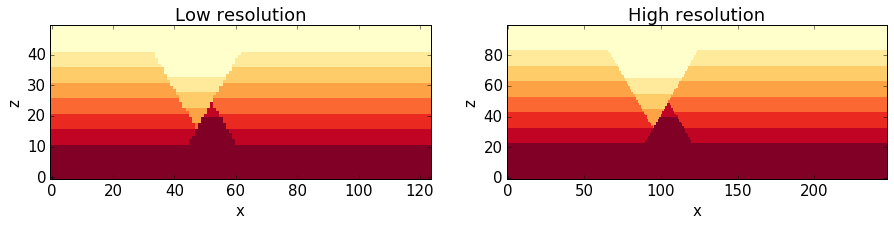
\includegraphics{2-Adjust-input_20_0.png}
\caption{png}\end{figure}

Note: the following two subsections contain some slighly advanced
examples on how to use the possibility to adjust cell sizes through
scripts directly to autmote processes that are infeasible using the GUI
version of Noddy - as a `peek preview' of the automation for uncertainty
estimation that follows in a later section. Feel free to skip those two
sections if you are only interested in the basic features so far.


\section{Estimating computation time for a high-resolution model}
\label{notebooks/2-Adjust-input:estimating-computation-time-for-a-high-resolution-model}
You surely realised (if you ran these examples in an actual interactive
ipython notebook) that the computation of the high-resolution model
takes siginificantly longer than the low-resolution model. In a
practical case, this can be very important.

\begin{Verbatim}[commandchars=\\\{\}]
\PYG{c}{\PYGZsh{} We use here simply the time() function to evaulate the simualtion time.}
\PYG{c}{\PYGZsh{} This is not the best possible way to do it, but probably the simplest.}
\PYG{k+kn}{import} \PYG{n+nn}{time}
\PYG{n}{start\PYGZus{}time} \PYG{o}{=} \PYG{n}{time}\PYG{o}{.}\PYG{n}{time}\PYG{p}{(}\PYG{p}{)}
\PYG{n}{pynoddy}\PYG{o}{.}\PYG{n}{compute\PYGZus{}model}\PYG{p}{(}\PYG{n}{history}\PYG{p}{,} \PYG{n}{output\PYGZus{}name}\PYG{p}{)}
\PYG{n}{end\PYGZus{}time} \PYG{o}{=} \PYG{n}{time}\PYG{o}{.}\PYG{n}{time}\PYG{p}{(}\PYG{p}{)}

\PYG{k}{print}\PYG{p}{(}\PYG{l+s}{\PYGZdq{}}\PYG{l+s}{Simulation time for low\PYGZhy{}resolution model: }\PYG{l+s+si}{\PYGZpc{}5.2f}\PYG{l+s}{ seconds}\PYG{l+s}{\PYGZdq{}} \PYG{o}{\PYGZpc{}} \PYG{p}{(}\PYG{n}{end\PYGZus{}time} \PYG{o}{\PYGZhy{}} \PYG{n}{start\PYGZus{}time}\PYG{p}{)}\PYG{p}{)}

\PYG{n}{start\PYGZus{}time} \PYG{o}{=} \PYG{n}{time}\PYG{o}{.}\PYG{n}{time}\PYG{p}{(}\PYG{p}{)}
\PYG{n}{pynoddy}\PYG{o}{.}\PYG{n}{compute\PYGZus{}model}\PYG{p}{(}\PYG{n}{new\PYGZus{}history}\PYG{p}{,} \PYG{n}{new\PYGZus{}output\PYGZus{}name}\PYG{p}{)}
\PYG{n}{end\PYGZus{}time} \PYG{o}{=} \PYG{n}{time}\PYG{o}{.}\PYG{n}{time}\PYG{p}{(}\PYG{p}{)}

\PYG{k}{print}\PYG{p}{(}\PYG{l+s}{\PYGZdq{}}\PYG{l+s}{Simulation time for high\PYGZhy{}resolution model: }\PYG{l+s+si}{\PYGZpc{}5.2f}\PYG{l+s}{ seconds}\PYG{l+s}{\PYGZdq{}} \PYG{o}{\PYGZpc{}} \PYG{p}{(}\PYG{n}{end\PYGZus{}time} \PYG{o}{\PYGZhy{}} \PYG{n}{start\PYGZus{}time}\PYG{p}{)}\PYG{p}{)}
\end{Verbatim}

\begin{Verbatim}[commandchars=\\\{\}]
Simulation time for low\PYGZhy{}resolution model:  0.73 seconds
Simulation time for high\PYGZhy{}resolution model:  5.78 seconds
\end{Verbatim}

For an estimation of required computing time for a given discretisation,
let's evaulate the time for a couple of steps, plot, and extrapolate:

\begin{Verbatim}[commandchars=\\\{\}]
\PYG{c}{\PYGZsh{} perform computation for a range of cube sizes}
\PYG{n}{cube\PYGZus{}sizes} \PYG{o}{=} \PYG{n}{np}\PYG{o}{.}\PYG{n}{arange}\PYG{p}{(}\PYG{l+m+mi}{200}\PYG{p}{,}\PYG{l+m+mi}{49}\PYG{p}{,}\PYG{o}{\PYGZhy{}}\PYG{l+m+mi}{5}\PYG{p}{)}
\PYG{n}{times} \PYG{o}{=} \PYG{p}{[}\PYG{p}{]}
\PYG{n}{NH1} \PYG{o}{=} \PYG{n}{pynoddy}\PYG{o}{.}\PYG{n}{history}\PYG{o}{.}\PYG{n}{NoddyHistory}\PYG{p}{(}\PYG{n}{history}\PYG{p}{)}
\PYG{n}{tmp\PYGZus{}history} \PYG{o}{=} \PYG{l+s}{\PYGZdq{}}\PYG{l+s}{tmp\PYGZus{}history}\PYG{l+s}{\PYGZdq{}}
\PYG{n}{tmp\PYGZus{}output} \PYG{o}{=} \PYG{l+s}{\PYGZdq{}}\PYG{l+s}{tmp\PYGZus{}output}\PYG{l+s}{\PYGZdq{}}
\PYG{k}{for} \PYG{n}{cube\PYGZus{}size} \PYG{o+ow}{in} \PYG{n}{cube\PYGZus{}sizes}\PYG{p}{:}
    \PYG{n}{NH1}\PYG{o}{.}\PYG{n}{change\PYGZus{}cube\PYGZus{}size}\PYG{p}{(}\PYG{n}{cube\PYGZus{}size}\PYG{p}{)}
    \PYG{n}{NH1}\PYG{o}{.}\PYG{n}{write\PYGZus{}history}\PYG{p}{(}\PYG{n}{tmp\PYGZus{}history}\PYG{p}{)}
    \PYG{n}{start\PYGZus{}time} \PYG{o}{=} \PYG{n}{time}\PYG{o}{.}\PYG{n}{time}\PYG{p}{(}\PYG{p}{)}
    \PYG{n}{pynoddy}\PYG{o}{.}\PYG{n}{compute\PYGZus{}model}\PYG{p}{(}\PYG{n}{tmp\PYGZus{}history}\PYG{p}{,} \PYG{n}{tmp\PYGZus{}output}\PYG{p}{)}
    \PYG{n}{end\PYGZus{}time} \PYG{o}{=} \PYG{n}{time}\PYG{o}{.}\PYG{n}{time}\PYG{p}{(}\PYG{p}{)}
    \PYG{n}{times}\PYG{o}{.}\PYG{n}{append}\PYG{p}{(}\PYG{n}{end\PYGZus{}time} \PYG{o}{\PYGZhy{}} \PYG{n}{start\PYGZus{}time}\PYG{p}{)}
\PYG{n}{times} \PYG{o}{=} \PYG{n}{np}\PYG{o}{.}\PYG{n}{array}\PYG{p}{(}\PYG{n}{times}\PYG{p}{)}
\end{Verbatim}

\begin{Verbatim}[commandchars=\\\{\}]
\PYG{c}{\PYGZsh{} create plot}
\PYG{n}{fig} \PYG{o}{=} \PYG{n}{plt}\PYG{o}{.}\PYG{n}{figure}\PYG{p}{(}\PYG{n}{figsize}\PYG{o}{=}\PYG{p}{(}\PYG{l+m+mi}{18}\PYG{p}{,}\PYG{l+m+mi}{4}\PYG{p}{)}\PYG{p}{)}
\PYG{n}{ax1} \PYG{o}{=} \PYG{n}{fig}\PYG{o}{.}\PYG{n}{add\PYGZus{}subplot}\PYG{p}{(}\PYG{l+m+mi}{131}\PYG{p}{)}
\PYG{n}{ax2} \PYG{o}{=} \PYG{n}{fig}\PYG{o}{.}\PYG{n}{add\PYGZus{}subplot}\PYG{p}{(}\PYG{l+m+mi}{132}\PYG{p}{)}
\PYG{n}{ax3} \PYG{o}{=} \PYG{n}{fig}\PYG{o}{.}\PYG{n}{add\PYGZus{}subplot}\PYG{p}{(}\PYG{l+m+mi}{133}\PYG{p}{)}

\PYG{n}{ax1}\PYG{o}{.}\PYG{n}{plot}\PYG{p}{(}\PYG{n}{cube\PYGZus{}sizes}\PYG{p}{,} \PYG{n}{np}\PYG{o}{.}\PYG{n}{array}\PYG{p}{(}\PYG{n}{times}\PYG{p}{)}\PYG{p}{,} \PYG{l+s}{\PYGZsq{}}\PYG{l+s}{ro\PYGZhy{}}\PYG{l+s}{\PYGZsq{}}\PYG{p}{)}
\PYG{n}{ax1}\PYG{o}{.}\PYG{n}{set\PYGZus{}xlabel}\PYG{p}{(}\PYG{l+s}{\PYGZsq{}}\PYG{l+s}{cubesize [m]}\PYG{l+s}{\PYGZsq{}}\PYG{p}{)}
\PYG{n}{ax1}\PYG{o}{.}\PYG{n}{set\PYGZus{}ylabel}\PYG{p}{(}\PYG{l+s}{\PYGZsq{}}\PYG{l+s}{time [s]}\PYG{l+s}{\PYGZsq{}}\PYG{p}{)}
\PYG{n}{ax1}\PYG{o}{.}\PYG{n}{set\PYGZus{}title}\PYG{p}{(}\PYG{l+s}{\PYGZsq{}}\PYG{l+s}{Computation time}\PYG{l+s}{\PYGZsq{}}\PYG{p}{)}
\PYG{n}{ax1}\PYG{o}{.}\PYG{n}{set\PYGZus{}xlim}\PYG{p}{(}\PYG{n}{ax1}\PYG{o}{.}\PYG{n}{get\PYGZus{}xlim}\PYG{p}{(}\PYG{p}{)}\PYG{p}{[}\PYG{p}{:}\PYG{p}{:}\PYG{o}{\PYGZhy{}}\PYG{l+m+mi}{1}\PYG{p}{]}\PYG{p}{)}

\PYG{n}{ax2}\PYG{o}{.}\PYG{n}{plot}\PYG{p}{(}\PYG{n}{cube\PYGZus{}sizes}\PYG{p}{,} \PYG{n}{times}\PYG{o}{*}\PYG{o}{*}\PYG{p}{(}\PYG{l+m+mi}{1}\PYG{o}{/}\PYG{l+m+mf}{3.}\PYG{p}{)}\PYG{p}{,} \PYG{l+s}{\PYGZsq{}}\PYG{l+s}{bo\PYGZhy{}}\PYG{l+s}{\PYGZsq{}}\PYG{p}{)}
\PYG{n}{ax2}\PYG{o}{.}\PYG{n}{set\PYGZus{}xlabel}\PYG{p}{(}\PYG{l+s}{\PYGZsq{}}\PYG{l+s}{cubesize [m]}\PYG{l+s}{\PYGZsq{}}\PYG{p}{)}
\PYG{n}{ax2}\PYG{o}{.}\PYG{n}{set\PYGZus{}ylabel}\PYG{p}{(}\PYG{l+s}{\PYGZsq{}}\PYG{l+s}{(time [s])**(1/3)}\PYG{l+s}{\PYGZsq{}}\PYG{p}{)}
\PYG{n}{ax2}\PYG{o}{.}\PYG{n}{set\PYGZus{}title}\PYG{p}{(}\PYG{l+s}{\PYGZsq{}}\PYG{l+s}{Computation time (cuberoot)}\PYG{l+s}{\PYGZsq{}}\PYG{p}{)}
\PYG{n}{ax2}\PYG{o}{.}\PYG{n}{set\PYGZus{}xlim}\PYG{p}{(}\PYG{n}{ax2}\PYG{o}{.}\PYG{n}{get\PYGZus{}xlim}\PYG{p}{(}\PYG{p}{)}\PYG{p}{[}\PYG{p}{:}\PYG{p}{:}\PYG{o}{\PYGZhy{}}\PYG{l+m+mi}{1}\PYG{p}{]}\PYG{p}{)}

\PYG{n}{ax3}\PYG{o}{.}\PYG{n}{semilogy}\PYG{p}{(}\PYG{n}{cube\PYGZus{}sizes}\PYG{p}{,} \PYG{n}{times}\PYG{p}{,} \PYG{l+s}{\PYGZsq{}}\PYG{l+s}{go\PYGZhy{}}\PYG{l+s}{\PYGZsq{}}\PYG{p}{)}
\PYG{n}{ax3}\PYG{o}{.}\PYG{n}{set\PYGZus{}xlabel}\PYG{p}{(}\PYG{l+s}{\PYGZsq{}}\PYG{l+s}{cubesize [m]}\PYG{l+s}{\PYGZsq{}}\PYG{p}{)}
\PYG{n}{ax3}\PYG{o}{.}\PYG{n}{set\PYGZus{}ylabel}\PYG{p}{(}\PYG{l+s}{\PYGZsq{}}\PYG{l+s}{time [s]}\PYG{l+s}{\PYGZsq{}}\PYG{p}{)}
\PYG{n}{ax3}\PYG{o}{.}\PYG{n}{set\PYGZus{}title}\PYG{p}{(}\PYG{l+s}{\PYGZsq{}}\PYG{l+s}{Computation time (y\PYGZhy{}log)}\PYG{l+s}{\PYGZsq{}}\PYG{p}{)}
\PYG{n}{ax3}\PYG{o}{.}\PYG{n}{set\PYGZus{}xlim}\PYG{p}{(}\PYG{n}{ax3}\PYG{o}{.}\PYG{n}{get\PYGZus{}xlim}\PYG{p}{(}\PYG{p}{)}\PYG{p}{[}\PYG{p}{:}\PYG{p}{:}\PYG{o}{\PYGZhy{}}\PYG{l+m+mi}{1}\PYG{p}{]}\PYG{p}{)}
\end{Verbatim}

\begin{Verbatim}[commandchars=\\\{\}]
\PYG{p}{(}\PYG{l+m+mf}{200.0}\PYG{p}{,} \PYG{l+m+mf}{40.0}\PYG{p}{)}
\end{Verbatim}
\begin{figure}[htbp]
\centering
\capstart

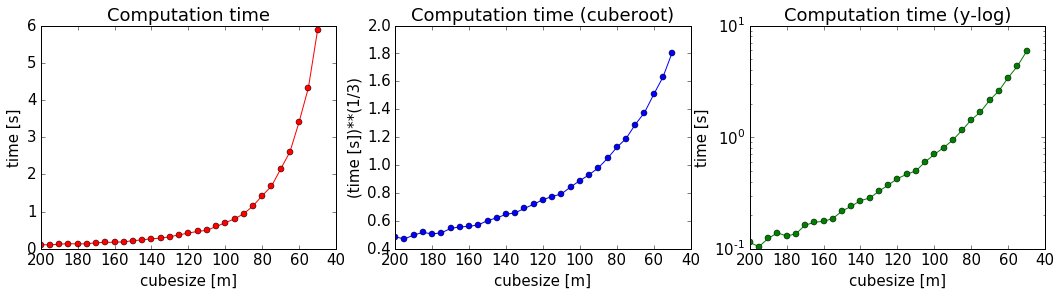
\includegraphics{2-Adjust-input_26_1.png}
\caption{png}\end{figure}

It is actually quite interesting that the computation time does not
scale with cubesize to the power of three (as could be expected, given
that we have a mesh in three dimensions). Or am I missing something?

Anyway, just because we can: let's assume that the scaling is somehow
exponential and try to fit a model for a time prediction. Given the last
plot, it looks like we could fit a logarithmic model with probably an
additional exponent (as the line is obviously not straight), so
something like:
\begin{gather}
\begin{split}f(x) = a + \left( b \log_{10}(x) \right)^{-c}\end{split}\notag
\end{gather}
Let's try to fit the curve with \code{scipy.optimize.curve\_fit}:

\begin{Verbatim}[commandchars=\\\{\}]
\PYG{c}{\PYGZsh{} perform curve fitting with scipy.optimize}
\PYG{k+kn}{import} \PYG{n+nn}{scipy.optimize}
\PYG{c}{\PYGZsh{} define function to be fit}
\PYG{k}{def} \PYG{n+nf}{func}\PYG{p}{(}\PYG{n}{x}\PYG{p}{,}\PYG{n}{a}\PYG{p}{,}\PYG{n}{b}\PYG{p}{,}\PYG{n}{c}\PYG{p}{)}\PYG{p}{:}
    \PYG{k}{return} \PYG{n}{a} \PYG{o}{+} \PYG{p}{(}\PYG{n}{b}\PYG{o}{*}\PYG{n}{np}\PYG{o}{.}\PYG{n}{log10}\PYG{p}{(}\PYG{n}{x}\PYG{p}{)}\PYG{p}{)}\PYG{o}{*}\PYG{o}{*}\PYG{p}{(}\PYG{o}{\PYGZhy{}}\PYG{n}{c}\PYG{p}{)}

\PYG{n}{popt}\PYG{p}{,} \PYG{n}{pcov} \PYG{o}{=} \PYG{n}{scipy}\PYG{o}{.}\PYG{n}{optimize}\PYG{o}{.}\PYG{n}{curve\PYGZus{}fit}\PYG{p}{(}\PYG{n}{func}\PYG{p}{,} \PYG{n}{cube\PYGZus{}sizes}\PYG{p}{,} \PYG{n}{np}\PYG{o}{.}\PYG{n}{array}\PYG{p}{(}\PYG{n}{times}\PYG{p}{)}\PYG{p}{,} \PYG{n}{p0} \PYG{o}{=} \PYG{p}{[}\PYG{o}{\PYGZhy{}}\PYG{l+m+mi}{1}\PYG{p}{,} \PYG{l+m+mf}{0.5}\PYG{p}{,} \PYG{l+m+mi}{2}\PYG{p}{]}\PYG{p}{)}
\PYG{n}{popt}
\end{Verbatim}

\begin{Verbatim}[commandchars=\\\{\}]
\PYG{n}{array}\PYG{p}{(}\PYG{p}{[} \PYG{o}{\PYGZhy{}}\PYG{l+m+mf}{0.05618538}\PYG{p}{,}   \PYG{l+m+mf}{0.50990774}\PYG{p}{,}  \PYG{l+m+mf}{12.45183398}\PYG{p}{]}\PYG{p}{)}
\end{Verbatim}

Interesting, it looks like Noody scales with something like:
\begin{gather}
\begin{split}f(x) = \left( 0.5 \log_{10}(x) \right)^{-12}\end{split}\notag
\end{gather}
\textbf{Note}: if you understand more about computational complexity than me,
it might not be that interesting to you at all - if this is the case,
please contact me and tell me why this result could be expected...

\begin{Verbatim}[commandchars=\\\{\}]
\PYG{n}{a}\PYG{p}{,}\PYG{n}{b}\PYG{p}{,}\PYG{n}{c} \PYG{o}{=} \PYG{n}{popt}
\PYG{n}{cube\PYGZus{}range} \PYG{o}{=} \PYG{n}{np}\PYG{o}{.}\PYG{n}{arange}\PYG{p}{(}\PYG{l+m+mi}{200}\PYG{p}{,}\PYG{l+m+mi}{20}\PYG{p}{,}\PYG{o}{\PYGZhy{}}\PYG{l+m+mi}{1}\PYG{p}{)}
\PYG{n}{times\PYGZus{}eval} \PYG{o}{=} \PYG{n}{func}\PYG{p}{(}\PYG{n}{cube\PYGZus{}range}\PYG{p}{,} \PYG{n}{a}\PYG{p}{,} \PYG{n}{b}\PYG{p}{,} \PYG{n}{c}\PYG{p}{)}
\PYG{n}{fig} \PYG{o}{=} \PYG{n}{plt}\PYG{o}{.}\PYG{n}{figure}\PYG{p}{(}\PYG{p}{)}
\PYG{n}{ax} \PYG{o}{=} \PYG{n}{fig}\PYG{o}{.}\PYG{n}{add\PYGZus{}subplot}\PYG{p}{(}\PYG{l+m+mi}{111}\PYG{p}{)}
\PYG{n}{ax}\PYG{o}{.}\PYG{n}{semilogy}\PYG{p}{(}\PYG{n}{cube\PYGZus{}range}\PYG{p}{,} \PYG{n}{times\PYGZus{}eval}\PYG{p}{,} \PYG{l+s}{\PYGZsq{}}\PYG{l+s}{\PYGZhy{}}\PYG{l+s}{\PYGZsq{}}\PYG{p}{)}
\PYG{n}{ax}\PYG{o}{.}\PYG{n}{semilogy}\PYG{p}{(}\PYG{n}{cube\PYGZus{}sizes}\PYG{p}{,} \PYG{n}{times}\PYG{p}{,} \PYG{l+s}{\PYGZsq{}}\PYG{l+s}{ko}\PYG{l+s}{\PYGZsq{}}\PYG{p}{)}
\PYG{c}{\PYGZsh{} reverse x\PYGZhy{}axis}
\PYG{n}{ax}\PYG{o}{.}\PYG{n}{set\PYGZus{}xlim}\PYG{p}{(}\PYG{n}{ax}\PYG{o}{.}\PYG{n}{get\PYGZus{}xlim}\PYG{p}{(}\PYG{p}{)}\PYG{p}{[}\PYG{p}{:}\PYG{p}{:}\PYG{o}{\PYGZhy{}}\PYG{l+m+mi}{1}\PYG{p}{]}\PYG{p}{)}
\end{Verbatim}

\begin{Verbatim}[commandchars=\\\{\}]
\PYG{p}{(}\PYG{l+m+mf}{200.0}\PYG{p}{,} \PYG{l+m+mf}{20.0}\PYG{p}{)}
\end{Verbatim}
\begin{figure}[htbp]
\centering
\capstart

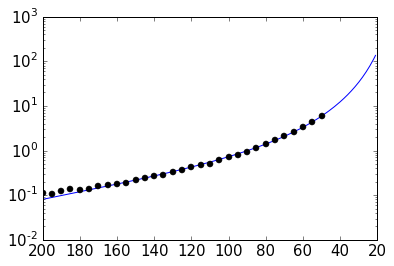
\includegraphics{2-Adjust-input_30_1.png}
\caption{png}\end{figure}

Not too bad... let's evaluate the time for a cube size of 40 m:

\begin{Verbatim}[commandchars=\\\{\}]
\PYG{n}{cube\PYGZus{}size} \PYG{o}{=} \PYG{l+m+mi}{40} \PYG{c}{\PYGZsh{} m}
\PYG{n}{time\PYGZus{}est} \PYG{o}{=} \PYG{n}{func}\PYG{p}{(}\PYG{n}{cube\PYGZus{}size}\PYG{p}{,} \PYG{n}{a}\PYG{p}{,} \PYG{n}{b}\PYG{p}{,} \PYG{n}{c}\PYG{p}{)}
\PYG{k}{print}\PYG{p}{(}\PYG{l+s}{\PYGZdq{}}\PYG{l+s}{Estimated time for a cube size of }\PYG{l+s+si}{\PYGZpc{}d}\PYG{l+s}{ m: }\PYG{l+s+si}{\PYGZpc{}.1f}\PYG{l+s}{ seconds}\PYG{l+s}{\PYGZdq{}} \PYG{o}{\PYGZpc{}} \PYG{p}{(}\PYG{n}{cube\PYGZus{}size}\PYG{p}{,} \PYG{n}{time\PYGZus{}est}\PYG{p}{)}\PYG{p}{)}
\end{Verbatim}

\begin{Verbatim}[commandchars=\\\{\}]
Estimated time for a cube size of 40 m: 12.4 seconds
\end{Verbatim}

Now let's check the actual simulation time:

\begin{Verbatim}[commandchars=\\\{\}]
\PYG{n}{NH1}\PYG{o}{.}\PYG{n}{change\PYGZus{}cube\PYGZus{}size}\PYG{p}{(}\PYG{n}{cube\PYGZus{}size}\PYG{p}{)}
\PYG{n}{NH1}\PYG{o}{.}\PYG{n}{write\PYGZus{}history}\PYG{p}{(}\PYG{n}{tmp\PYGZus{}history}\PYG{p}{)}
\PYG{n}{start\PYGZus{}time} \PYG{o}{=} \PYG{n}{time}\PYG{o}{.}\PYG{n}{time}\PYG{p}{(}\PYG{p}{)}
\PYG{n}{pynoddy}\PYG{o}{.}\PYG{n}{compute\PYGZus{}model}\PYG{p}{(}\PYG{n}{tmp\PYGZus{}history}\PYG{p}{,} \PYG{n}{tmp\PYGZus{}output}\PYG{p}{)}
\PYG{n}{end\PYGZus{}time} \PYG{o}{=} \PYG{n}{time}\PYG{o}{.}\PYG{n}{time}\PYG{p}{(}\PYG{p}{)}
\PYG{n}{time\PYGZus{}comp} \PYG{o}{=} \PYG{n}{end\PYGZus{}time} \PYG{o}{\PYGZhy{}} \PYG{n}{start\PYGZus{}time}

\PYG{k}{print}\PYG{p}{(}\PYG{l+s}{\PYGZdq{}}\PYG{l+s}{Actual computation time for a cube size of }\PYG{l+s+si}{\PYGZpc{}d}\PYG{l+s}{ m: }\PYG{l+s+si}{\PYGZpc{}.1f}\PYG{l+s}{ seconds}\PYG{l+s}{\PYGZdq{}} \PYG{o}{\PYGZpc{}} \PYG{p}{(}\PYG{n}{cube\PYGZus{}size}\PYG{p}{,} \PYG{n}{time\PYGZus{}comp}\PYG{p}{)}\PYG{p}{)}
\end{Verbatim}

\begin{Verbatim}[commandchars=\\\{\}]
Actual computation time for a cube size of 40 m: 11.6 seconds
\end{Verbatim}

Not too bad, probably in the range of the inherent variability... and if
we check it in the plot:

\begin{Verbatim}[commandchars=\\\{\}]
\PYG{n}{fig} \PYG{o}{=} \PYG{n}{plt}\PYG{o}{.}\PYG{n}{figure}\PYG{p}{(}\PYG{p}{)}
\PYG{n}{ax} \PYG{o}{=} \PYG{n}{fig}\PYG{o}{.}\PYG{n}{add\PYGZus{}subplot}\PYG{p}{(}\PYG{l+m+mi}{111}\PYG{p}{)}
\PYG{n}{ax}\PYG{o}{.}\PYG{n}{semilogy}\PYG{p}{(}\PYG{n}{cube\PYGZus{}range}\PYG{p}{,} \PYG{n}{times\PYGZus{}eval}\PYG{p}{,} \PYG{l+s}{\PYGZsq{}}\PYG{l+s}{\PYGZhy{}}\PYG{l+s}{\PYGZsq{}}\PYG{p}{)}
\PYG{n}{ax}\PYG{o}{.}\PYG{n}{semilogy}\PYG{p}{(}\PYG{n}{cube\PYGZus{}sizes}\PYG{p}{,} \PYG{n}{times}\PYG{p}{,} \PYG{l+s}{\PYGZsq{}}\PYG{l+s}{ko}\PYG{l+s}{\PYGZsq{}}\PYG{p}{)}
\PYG{n}{ax}\PYG{o}{.}\PYG{n}{semilogy}\PYG{p}{(}\PYG{n}{cube\PYGZus{}size}\PYG{p}{,} \PYG{n}{time\PYGZus{}comp}\PYG{p}{,} \PYG{l+s}{\PYGZsq{}}\PYG{l+s}{ro}\PYG{l+s}{\PYGZsq{}}\PYG{p}{)}
\PYG{c}{\PYGZsh{} reverse x\PYGZhy{}axis}
\PYG{n}{ax}\PYG{o}{.}\PYG{n}{set\PYGZus{}xlim}\PYG{p}{(}\PYG{n}{ax}\PYG{o}{.}\PYG{n}{get\PYGZus{}xlim}\PYG{p}{(}\PYG{p}{)}\PYG{p}{[}\PYG{p}{:}\PYG{p}{:}\PYG{o}{\PYGZhy{}}\PYG{l+m+mi}{1}\PYG{p}{]}\PYG{p}{)}
\end{Verbatim}

\begin{Verbatim}[commandchars=\\\{\}]
\PYG{p}{(}\PYG{l+m+mf}{200.0}\PYG{p}{,} \PYG{l+m+mf}{20.0}\PYG{p}{)}
\end{Verbatim}
\begin{figure}[htbp]
\centering
\capstart

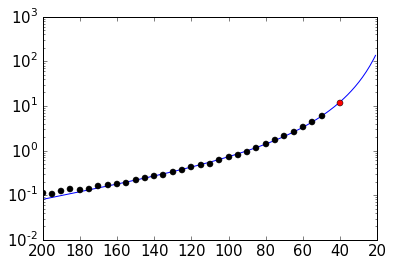
\includegraphics{2-Adjust-input_36_1.png}
\caption{png}\end{figure}

Anyway, the point of this excercise was not a precise evaluation of
Noddy's computational complexity, but to provide a simple means of
evaluating computation time for a high resolution model, using the
flexibility of writing simple scripts using pynoddy, and a couple of
additional python modules.

For a realistic case, it should, of course, be sufficient to determine
the time based on a lot less computed points. If you like, test it with
your favourite model and tell me if it proved useful (or not)!


\section{Simple convergence study}
\label{notebooks/2-Adjust-input:simple-convergence-study}
So: why would we want to run a high-resolution model, anyway? Well, of
course, it produces nicer pictures - but on a scientific level, that's
completely irrelevant (haha, not true - so nice if it would be...).

Anyway, if we want to use the model in a scientific study, for example
to evaluate volume of specific units, or to estimate the geological
topology (Mark is working on this topic with some cool ideas - example
to be implemented here, ``soon''), we want to know if the resolution of
the model is actually high enough to produce meaningful results.

As a simple example of the evaluation of model resolution, we will here
inlcude a volume convergence study, i.e. we will estimate at which level
of increasing model resolution the estimated block volumes do not change
anymore.

The entire procedure is very similar to the computational time
evaluation above, only that we now also analyse the output and determine
the rock volumes of each defined geological unit:

\begin{Verbatim}[commandchars=\\\{\}]
\PYG{c}{\PYGZsh{} perform computation for a range of cube sizes}
\PYG{n+nb}{reload}\PYG{p}{(}\PYG{n}{pynoddy}\PYG{o}{.}\PYG{n}{output}\PYG{p}{)}
\PYG{n}{cube\PYGZus{}sizes} \PYG{o}{=} \PYG{n}{np}\PYG{o}{.}\PYG{n}{arange}\PYG{p}{(}\PYG{l+m+mi}{200}\PYG{p}{,}\PYG{l+m+mi}{49}\PYG{p}{,}\PYG{o}{\PYGZhy{}}\PYG{l+m+mi}{5}\PYG{p}{)}
\PYG{n}{all\PYGZus{}volumes} \PYG{o}{=} \PYG{p}{[}\PYG{p}{]}
\PYG{n}{N\PYGZus{}tmp} \PYG{o}{=} \PYG{n}{pynoddy}\PYG{o}{.}\PYG{n}{history}\PYG{o}{.}\PYG{n}{NoddyHistory}\PYG{p}{(}\PYG{n}{history}\PYG{p}{)}
\PYG{n}{tmp\PYGZus{}history} \PYG{o}{=} \PYG{l+s}{\PYGZdq{}}\PYG{l+s}{tmp\PYGZus{}history}\PYG{l+s}{\PYGZdq{}}
\PYG{n}{tmp\PYGZus{}output} \PYG{o}{=} \PYG{l+s}{\PYGZdq{}}\PYG{l+s}{tmp\PYGZus{}output}\PYG{l+s}{\PYGZdq{}}
\PYG{k}{for} \PYG{n}{cube\PYGZus{}size} \PYG{o+ow}{in} \PYG{n}{cube\PYGZus{}sizes}\PYG{p}{:}
    \PYG{c}{\PYGZsh{} adjust cube size}
    \PYG{n}{N\PYGZus{}tmp}\PYG{o}{.}\PYG{n}{change\PYGZus{}cube\PYGZus{}size}\PYG{p}{(}\PYG{n}{cube\PYGZus{}size}\PYG{p}{)}
    \PYG{n}{N\PYGZus{}tmp}\PYG{o}{.}\PYG{n}{write\PYGZus{}history}\PYG{p}{(}\PYG{n}{tmp\PYGZus{}history}\PYG{p}{)}
    \PYG{n}{pynoddy}\PYG{o}{.}\PYG{n}{compute\PYGZus{}model}\PYG{p}{(}\PYG{n}{tmp\PYGZus{}history}\PYG{p}{,} \PYG{n}{tmp\PYGZus{}output}\PYG{p}{)}
    \PYG{c}{\PYGZsh{} open simulated model and determine volumes}
    \PYG{n}{O\PYGZus{}tmp} \PYG{o}{=} \PYG{n}{pynoddy}\PYG{o}{.}\PYG{n}{output}\PYG{o}{.}\PYG{n}{NoddyOutput}\PYG{p}{(}\PYG{n}{tmp\PYGZus{}output}\PYG{p}{)}
    \PYG{n}{O\PYGZus{}tmp}\PYG{o}{.}\PYG{n}{determine\PYGZus{}unit\PYGZus{}volumes}\PYG{p}{(}\PYG{p}{)}
    \PYG{n}{all\PYGZus{}volumes}\PYG{o}{.}\PYG{n}{append}\PYG{p}{(}\PYG{n}{O\PYGZus{}tmp}\PYG{o}{.}\PYG{n}{unit\PYGZus{}volumes}\PYG{p}{)}
\end{Verbatim}

\begin{Verbatim}[commandchars=\\\{\}]
\PYG{n}{all\PYGZus{}volumes} \PYG{o}{=} \PYG{n}{np}\PYG{o}{.}\PYG{n}{array}\PYG{p}{(}\PYG{n}{all\PYGZus{}volumes}\PYG{p}{)}
\PYG{n}{fig} \PYG{o}{=} \PYG{n}{plt}\PYG{o}{.}\PYG{n}{figure}\PYG{p}{(}\PYG{n}{figsize}\PYG{o}{=}\PYG{p}{(}\PYG{l+m+mi}{16}\PYG{p}{,}\PYG{l+m+mi}{4}\PYG{p}{)}\PYG{p}{)}
\PYG{n}{ax1} \PYG{o}{=} \PYG{n}{fig}\PYG{o}{.}\PYG{n}{add\PYGZus{}subplot}\PYG{p}{(}\PYG{l+m+mi}{121}\PYG{p}{)}
\PYG{n}{ax2} \PYG{o}{=} \PYG{n}{fig}\PYG{o}{.}\PYG{n}{add\PYGZus{}subplot}\PYG{p}{(}\PYG{l+m+mi}{122}\PYG{p}{)}

\PYG{c}{\PYGZsh{} separate into two plots for better visibility:}
\PYG{k}{for} \PYG{n}{i} \PYG{o+ow}{in} \PYG{n+nb}{range}\PYG{p}{(}\PYG{n}{np}\PYG{o}{.}\PYG{n}{shape}\PYG{p}{(}\PYG{n}{all\PYGZus{}volumes}\PYG{p}{)}\PYG{p}{[}\PYG{l+m+mi}{1}\PYG{p}{]}\PYG{p}{)}\PYG{p}{:}
    \PYG{k}{if} \PYG{n}{i} \PYG{o}{\PYGZlt{}} \PYG{l+m+mi}{4}\PYG{p}{:}
        \PYG{n}{ax1}\PYG{o}{.}\PYG{n}{plot}\PYG{p}{(}\PYG{n}{cube\PYGZus{}sizes}\PYG{p}{,} \PYG{n}{all\PYGZus{}volumes}\PYG{p}{[}\PYG{p}{:}\PYG{p}{,}\PYG{n}{i}\PYG{p}{]}\PYG{p}{,} \PYG{l+s}{\PYGZsq{}}\PYG{l+s}{o\PYGZhy{}}\PYG{l+s}{\PYGZsq{}}\PYG{p}{,} \PYG{n}{label}\PYG{o}{=}\PYG{l+s}{\PYGZsq{}}\PYG{l+s}{unit }\PYG{l+s+si}{\PYGZpc{}d}\PYG{l+s}{\PYGZsq{}} \PYG{o}{\PYGZpc{}}\PYG{n}{i}\PYG{p}{)}
    \PYG{k}{else}\PYG{p}{:}
        \PYG{n}{ax2}\PYG{o}{.}\PYG{n}{plot}\PYG{p}{(}\PYG{n}{cube\PYGZus{}sizes}\PYG{p}{,} \PYG{n}{all\PYGZus{}volumes}\PYG{p}{[}\PYG{p}{:}\PYG{p}{,}\PYG{n}{i}\PYG{p}{]}\PYG{p}{,} \PYG{l+s}{\PYGZsq{}}\PYG{l+s}{o\PYGZhy{}}\PYG{l+s}{\PYGZsq{}}\PYG{p}{,} \PYG{n}{label}\PYG{o}{=}\PYG{l+s}{\PYGZsq{}}\PYG{l+s}{unit }\PYG{l+s+si}{\PYGZpc{}d}\PYG{l+s}{\PYGZsq{}} \PYG{o}{\PYGZpc{}}\PYG{n}{i}\PYG{p}{)}

\PYG{n}{ax1}\PYG{o}{.}\PYG{n}{legend}\PYG{p}{(}\PYG{n}{loc}\PYG{o}{=}\PYG{l+m+mi}{2}\PYG{p}{)}
\PYG{n}{ax2}\PYG{o}{.}\PYG{n}{legend}\PYG{p}{(}\PYG{n}{loc}\PYG{o}{=}\PYG{l+m+mi}{2}\PYG{p}{)}
\PYG{c}{\PYGZsh{} reverse axes}
\PYG{n}{ax1}\PYG{o}{.}\PYG{n}{set\PYGZus{}xlim}\PYG{p}{(}\PYG{n}{ax1}\PYG{o}{.}\PYG{n}{get\PYGZus{}xlim}\PYG{p}{(}\PYG{p}{)}\PYG{p}{[}\PYG{p}{:}\PYG{p}{:}\PYG{o}{\PYGZhy{}}\PYG{l+m+mi}{1}\PYG{p}{]}\PYG{p}{)}
\PYG{n}{ax2}\PYG{o}{.}\PYG{n}{set\PYGZus{}xlim}\PYG{p}{(}\PYG{n}{ax2}\PYG{o}{.}\PYG{n}{get\PYGZus{}xlim}\PYG{p}{(}\PYG{p}{)}\PYG{p}{[}\PYG{p}{:}\PYG{p}{:}\PYG{o}{\PYGZhy{}}\PYG{l+m+mi}{1}\PYG{p}{]}\PYG{p}{)}

\PYG{n}{ax1}\PYG{o}{.}\PYG{n}{set\PYGZus{}xlabel}\PYG{p}{(}\PYG{l+s}{\PYGZdq{}}\PYG{l+s}{Block size [m]}\PYG{l+s}{\PYGZdq{}}\PYG{p}{)}
\PYG{n}{ax1}\PYG{o}{.}\PYG{n}{set\PYGZus{}ylabel}\PYG{p}{(}\PYG{l+s}{\PYGZdq{}}\PYG{l+s}{Total unit volume [m**3]}\PYG{l+s}{\PYGZdq{}}\PYG{p}{)}
\PYG{n}{ax2}\PYG{o}{.}\PYG{n}{set\PYGZus{}xlabel}\PYG{p}{(}\PYG{l+s}{\PYGZdq{}}\PYG{l+s}{Block size [m]}\PYG{l+s}{\PYGZdq{}}\PYG{p}{)}
\PYG{n}{ax2}\PYG{o}{.}\PYG{n}{set\PYGZus{}ylabel}\PYG{p}{(}\PYG{l+s}{\PYGZdq{}}\PYG{l+s}{Total unit volume [m**3]}\PYG{l+s}{\PYGZdq{}}\PYG{p}{)}
\end{Verbatim}

\begin{Verbatim}[commandchars=\\\{\}]
\PYGZlt{}matplotlib.text.Text at 0x107eb7250\PYGZgt{}
\end{Verbatim}
\begin{figure}[htbp]
\centering
\capstart

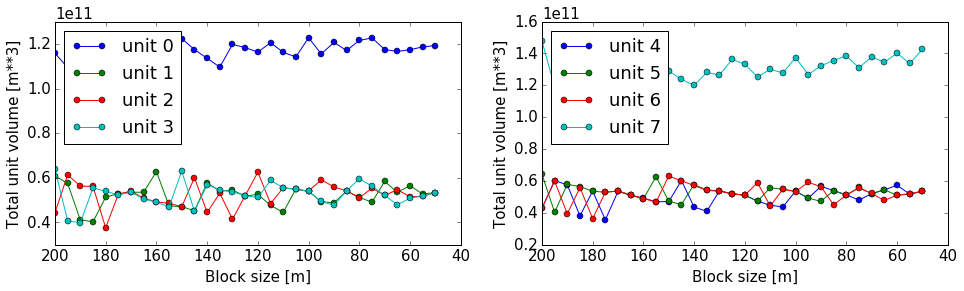
\includegraphics{2-Adjust-input_40_1.png}
\caption{png}\end{figure}

It looks like the volumes would start to converge from about a block
size of 100 m. The example model is pretty small and simple, probably
not the best example for this study. Try it out with your own, highly
complex, favourite pet model :-)


\chapter{Geological events in pynoddy: organisation and adpatiation}
\label{notebooks/3-Events:geological-events-in-pynoddy-organisation-and-adpatiation}\label{notebooks/3-Events::doc}
We will here describe how the single geological events of a Noddy
history are organised within pynoddy. We will then evaluate in some more
detail how aspects of events can be adapted and their effect evaluated.

\begin{Verbatim}[commandchars=\\\{\}]
\PYG{k+kn}{from} \PYG{n+nn}{IPython.core.display} \PYG{k+kn}{import} \PYG{n}{HTML}
\PYG{n}{css\PYGZus{}file} \PYG{o}{=} \PYG{l+s}{\PYGZsq{}}\PYG{l+s}{pynoddy.css}\PYG{l+s}{\PYGZsq{}}
\PYG{n}{HTML}\PYG{p}{(}\PYG{n+nb}{open}\PYG{p}{(}\PYG{n}{css\PYGZus{}file}\PYG{p}{,} \PYG{l+s}{\PYGZdq{}}\PYG{l+s}{r}\PYG{l+s}{\PYGZdq{}}\PYG{p}{)}\PYG{o}{.}\PYG{n}{read}\PYG{p}{(}\PYG{p}{)}\PYG{p}{)}
\end{Verbatim}

\begin{Verbatim}[commandchars=\\\{\}]
\PYGZpc{}matplotlib inline
\end{Verbatim}


\section{Loading events from a Noddy history}
\label{notebooks/3-Events:loading-events-from-a-noddy-history}
In the current set-up of pynoddy, we always start with a pre-defined
Noddy history loaded from a file, and then change aspects of the history
and the single events. The first step is therefore to load the history
file and to extract the single geological events. This is done
automatically as default when loading the history file into the History
object:

\begin{Verbatim}[commandchars=\\\{\}]
\PYG{k+kn}{import} \PYG{n+nn}{sys}\PYG{o}{,} \PYG{n+nn}{os}
\PYG{k+kn}{import} \PYG{n+nn}{matplotlib.pyplot} \PYG{k+kn}{as} \PYG{n+nn}{plt}
\PYG{c}{\PYGZsh{} adjust some settings for matplotlib}
\PYG{k+kn}{from} \PYG{n+nn}{matplotlib} \PYG{k+kn}{import} \PYG{n}{rcParams}
\PYG{c}{\PYGZsh{} print rcParams}
\PYG{n}{rcParams}\PYG{p}{[}\PYG{l+s}{\PYGZsq{}}\PYG{l+s}{font.size}\PYG{l+s}{\PYGZsq{}}\PYG{p}{]} \PYG{o}{=} \PYG{l+m+mi}{15}
\PYG{c}{\PYGZsh{} determine path of repository to set paths corretly below}
\PYG{n}{repo\PYGZus{}path} \PYG{o}{=} \PYG{n}{os}\PYG{o}{.}\PYG{n}{path}\PYG{o}{.}\PYG{n}{realpath}\PYG{p}{(}\PYG{l+s}{\PYGZsq{}}\PYG{l+s}{../..}\PYG{l+s}{\PYGZsq{}}\PYG{p}{)}

\PYG{k+kn}{import} \PYG{n+nn}{pynoddy}
\PYG{k+kn}{import} \PYG{n+nn}{pynoddy.history}
\PYG{k+kn}{import} \PYG{n+nn}{pynoddy.events}
\PYG{k+kn}{import} \PYG{n+nn}{pynoddy.output}
\PYG{n+nb}{reload}\PYG{p}{(}\PYG{n}{pynoddy}\PYG{p}{)}
\end{Verbatim}

\begin{Verbatim}[commandchars=\\\{\}]
\PYGZlt{}module \PYGZsq{}pynoddy\PYGZsq{} from \PYGZsq{}/Users/flow/git/pynoddy/pynoddy/\PYGZus{}\PYGZus{}init\PYGZus{}\PYGZus{}.pyc\PYGZsq{}\PYGZgt{}
\end{Verbatim}

\begin{Verbatim}[commandchars=\\\{\}]
\PYG{c}{\PYGZsh{} Change to sandbox directory to store results}
\PYG{n}{os}\PYG{o}{.}\PYG{n}{chdir}\PYG{p}{(}\PYG{n}{os}\PYG{o}{.}\PYG{n}{path}\PYG{o}{.}\PYG{n}{join}\PYG{p}{(}\PYG{n}{repo\PYGZus{}path}\PYG{p}{,} \PYG{l+s}{\PYGZsq{}}\PYG{l+s}{sandbox}\PYG{l+s}{\PYGZsq{}}\PYG{p}{)}\PYG{p}{)}

\PYG{c}{\PYGZsh{} Path to exmaple directory in this repository}
\PYG{n}{example\PYGZus{}directory} \PYG{o}{=} \PYG{n}{os}\PYG{o}{.}\PYG{n}{path}\PYG{o}{.}\PYG{n}{join}\PYG{p}{(}\PYG{n}{repo\PYGZus{}path}\PYG{p}{,}\PYG{l+s}{\PYGZsq{}}\PYG{l+s}{examples}\PYG{l+s}{\PYGZsq{}}\PYG{p}{)}
\PYG{c}{\PYGZsh{} Compute noddy model for history file}
\PYG{n}{history} \PYG{o}{=} \PYG{l+s}{\PYGZsq{}}\PYG{l+s}{simple\PYGZus{}two\PYGZus{}faults.his}\PYG{l+s}{\PYGZsq{}}
\PYG{n}{history\PYGZus{}ori} \PYG{o}{=} \PYG{n}{os}\PYG{o}{.}\PYG{n}{path}\PYG{o}{.}\PYG{n}{join}\PYG{p}{(}\PYG{n}{example\PYGZus{}directory}\PYG{p}{,} \PYG{n}{history}\PYG{p}{)}
\PYG{n}{output\PYGZus{}name} \PYG{o}{=} \PYG{l+s}{\PYGZsq{}}\PYG{l+s}{noddy\PYGZus{}out}\PYG{l+s}{\PYGZsq{}}
\PYG{n+nb}{reload}\PYG{p}{(}\PYG{n}{pynoddy}\PYG{o}{.}\PYG{n}{history}\PYG{p}{)}
\PYG{n+nb}{reload}\PYG{p}{(}\PYG{n}{pynoddy}\PYG{o}{.}\PYG{n}{events}\PYG{p}{)}
\PYG{n}{H1} \PYG{o}{=} \PYG{n}{pynoddy}\PYG{o}{.}\PYG{n}{history}\PYG{o}{.}\PYG{n}{NoddyHistory}\PYG{p}{(}\PYG{n}{history\PYGZus{}ori}\PYG{p}{)}
\PYG{c}{\PYGZsh{} Before we do anything else, let\PYGZsq{}s actually define the cube size here to}
\PYG{c}{\PYGZsh{} adjust the resolution for all subsequent examples}
\PYG{n}{H1}\PYG{o}{.}\PYG{n}{change\PYGZus{}cube\PYGZus{}size}\PYG{p}{(}\PYG{l+m+mi}{100}\PYG{p}{)}
\PYG{c}{\PYGZsh{} compute model \PYGZhy{} note: not strictly required, here just to ensure changed cube size}
\PYG{n}{H1}\PYG{o}{.}\PYG{n}{write\PYGZus{}history}\PYG{p}{(}\PYG{n}{history}\PYG{p}{)}
\PYG{n}{pynoddy}\PYG{o}{.}\PYG{n}{compute\PYGZus{}model}\PYG{p}{(}\PYG{n}{history}\PYG{p}{,} \PYG{n}{output\PYGZus{}name}\PYG{p}{)}
\end{Verbatim}

\begin{Verbatim}[commandchars=\\\{\}]
\PYG{l+s}{\PYGZsq{}}\PYG{l+s}{\PYGZsq{}}
\end{Verbatim}

Events are stored in the object dictionary ``events'' (who would have
thought), where the key corresponds to the position in the timeline:

\begin{Verbatim}[commandchars=\\\{\}]
\PYG{n}{H1}\PYG{o}{.}\PYG{n}{events}
\end{Verbatim}

\begin{Verbatim}[commandchars=\\\{\}]
\PYGZob{}1: \PYGZlt{}pynoddy.events.Stratigraphy at 0x10cf2b410\PYGZgt{},
 2: \PYGZlt{}pynoddy.events.Fault at 0x10cf2b450\PYGZgt{},
 3: \PYGZlt{}pynoddy.events.Fault at 0x10cf2b490\PYGZgt{}\PYGZcb{}
\end{Verbatim}

We can see here that three events are defined in the history. Events are
organised as objects themselves, containing all the relevant properties
and information about the events. For example, the second fault event is
defined as:

\begin{Verbatim}[commandchars=\\\{\}]
\PYG{n}{H1}\PYG{o}{.}\PYG{n}{events}\PYG{p}{[}\PYG{l+m+mi}{3}\PYG{p}{]}\PYG{o}{.}\PYG{n}{properties}
\end{Verbatim}

\begin{Verbatim}[commandchars=\\\{\}]
\PYG{p}{\PYGZob{}}\PYG{l+s}{\PYGZsq{}}\PYG{l+s}{Amplitude}\PYG{l+s}{\PYGZsq{}}\PYG{p}{:} \PYG{l+m+mf}{2000.0}\PYG{p}{,}
 \PYG{l+s}{\PYGZsq{}}\PYG{l+s}{Blue}\PYG{l+s}{\PYGZsq{}}\PYG{p}{:} \PYG{l+m+mf}{0.0}\PYG{p}{,}
 \PYG{l+s}{\PYGZsq{}}\PYG{l+s}{Color Name}\PYG{l+s}{\PYGZsq{}}\PYG{p}{:} \PYG{l+s}{\PYGZsq{}}\PYG{l+s}{Custom Colour 5}\PYG{l+s}{\PYGZsq{}}\PYG{p}{,}
 \PYG{l+s}{\PYGZsq{}}\PYG{l+s}{Cyl Index}\PYG{l+s}{\PYGZsq{}}\PYG{p}{:} \PYG{l+m+mf}{0.0}\PYG{p}{,}
 \PYG{l+s}{\PYGZsq{}}\PYG{l+s}{Dip}\PYG{l+s}{\PYGZsq{}}\PYG{p}{:} \PYG{l+m+mf}{60.0}\PYG{p}{,}
 \PYG{l+s}{\PYGZsq{}}\PYG{l+s}{Dip Direction}\PYG{l+s}{\PYGZsq{}}\PYG{p}{:} \PYG{l+m+mf}{270.0}\PYG{p}{,}
 \PYG{l+s}{\PYGZsq{}}\PYG{l+s}{Geometry}\PYG{l+s}{\PYGZsq{}}\PYG{p}{:} \PYG{l+s}{\PYGZsq{}}\PYG{l+s}{Translation}\PYG{l+s}{\PYGZsq{}}\PYG{p}{,}
 \PYG{l+s}{\PYGZsq{}}\PYG{l+s}{Green}\PYG{l+s}{\PYGZsq{}}\PYG{p}{:} \PYG{l+m+mf}{0.0}\PYG{p}{,}
 \PYG{l+s}{\PYGZsq{}}\PYG{l+s}{Movement}\PYG{l+s}{\PYGZsq{}}\PYG{p}{:} \PYG{l+s}{\PYGZsq{}}\PYG{l+s}{Hanging Wall}\PYG{l+s}{\PYGZsq{}}\PYG{p}{,}
 \PYG{l+s}{\PYGZsq{}}\PYG{l+s}{Pitch}\PYG{l+s}{\PYGZsq{}}\PYG{p}{:} \PYG{l+m+mf}{90.0}\PYG{p}{,}
 \PYG{l+s}{\PYGZsq{}}\PYG{l+s}{Profile Pitch}\PYG{l+s}{\PYGZsq{}}\PYG{p}{:} \PYG{l+m+mf}{90.0}\PYG{p}{,}
 \PYG{l+s}{\PYGZsq{}}\PYG{l+s}{Radius}\PYG{l+s}{\PYGZsq{}}\PYG{p}{:} \PYG{l+m+mf}{1000.0}\PYG{p}{,}
 \PYG{l+s}{\PYGZsq{}}\PYG{l+s}{Red}\PYG{l+s}{\PYGZsq{}}\PYG{p}{:} \PYG{l+m+mf}{254.0}\PYG{p}{,}
 \PYG{l+s}{\PYGZsq{}}\PYG{l+s}{Rotation}\PYG{l+s}{\PYGZsq{}}\PYG{p}{:} \PYG{l+m+mf}{30.0}\PYG{p}{,}
 \PYG{l+s}{\PYGZsq{}}\PYG{l+s}{Slip}\PYG{l+s}{\PYGZsq{}}\PYG{p}{:} \PYG{l+m+mf}{1000.0}\PYG{p}{,}
 \PYG{l+s}{\PYGZsq{}}\PYG{l+s}{X}\PYG{l+s}{\PYGZsq{}}\PYG{p}{:} \PYG{l+m+mf}{5500.0}\PYG{p}{,}
 \PYG{l+s}{\PYGZsq{}}\PYG{l+s}{XAxis}\PYG{l+s}{\PYGZsq{}}\PYG{p}{:} \PYG{l+m+mf}{2000.0}\PYG{p}{,}
 \PYG{l+s}{\PYGZsq{}}\PYG{l+s}{Y}\PYG{l+s}{\PYGZsq{}}\PYG{p}{:} \PYG{l+m+mf}{7000.0}\PYG{p}{,}
 \PYG{l+s}{\PYGZsq{}}\PYG{l+s}{YAxis}\PYG{l+s}{\PYGZsq{}}\PYG{p}{:} \PYG{l+m+mf}{2000.0}\PYG{p}{,}
 \PYG{l+s}{\PYGZsq{}}\PYG{l+s}{Z}\PYG{l+s}{\PYGZsq{}}\PYG{p}{:} \PYG{l+m+mf}{5000.0}\PYG{p}{,}
 \PYG{l+s}{\PYGZsq{}}\PYG{l+s}{ZAxis}\PYG{l+s}{\PYGZsq{}}\PYG{p}{:} \PYG{l+m+mf}{2000.0}\PYG{p}{\PYGZcb{}}
\end{Verbatim}


\section{Changing aspects of geological events}
\label{notebooks/3-Events:changing-aspects-of-geological-events}
So what we now want to do, of course, is to change aspects of these
events and to evaluate the effect on the resulting geological model.
Parameters can directly be updated in the properties dictionary:

\begin{Verbatim}[commandchars=\\\{\}]
\PYG{n}{H1} \PYG{o}{=} \PYG{n}{pynoddy}\PYG{o}{.}\PYG{n}{history}\PYG{o}{.}\PYG{n}{NoddyHistory}\PYG{p}{(}\PYG{n}{history\PYGZus{}ori}\PYG{p}{)}
\PYG{c}{\PYGZsh{} get the original dip of the fault}
\PYG{n}{dip\PYGZus{}ori} \PYG{o}{=} \PYG{n}{H1}\PYG{o}{.}\PYG{n}{events}\PYG{p}{[}\PYG{l+m+mi}{3}\PYG{p}{]}\PYG{o}{.}\PYG{n}{properties}\PYG{p}{[}\PYG{l+s}{\PYGZsq{}}\PYG{l+s}{Dip}\PYG{l+s}{\PYGZsq{}}\PYG{p}{]}

\PYG{c}{\PYGZsh{} add 10 degrees to dip}
\PYG{n}{add\PYGZus{}dip} \PYG{o}{=} \PYG{o}{\PYGZhy{}}\PYG{l+m+mi}{10}
\PYG{n}{dip\PYGZus{}new} \PYG{o}{=} \PYG{n}{dip\PYGZus{}ori} \PYG{o}{+} \PYG{n}{add\PYGZus{}dip}

\PYG{c}{\PYGZsh{} and assign back to properties dictionary:}
\PYG{n}{H1}\PYG{o}{.}\PYG{n}{events}\PYG{p}{[}\PYG{l+m+mi}{3}\PYG{p}{]}\PYG{o}{.}\PYG{n}{properties}\PYG{p}{[}\PYG{l+s}{\PYGZsq{}}\PYG{l+s}{Dip}\PYG{l+s}{\PYGZsq{}}\PYG{p}{]} \PYG{o}{=} \PYG{n}{dip\PYGZus{}new}
\PYG{c}{\PYGZsh{} H1.events[2].properties[\PYGZsq{}Dip\PYGZsq{}] = dip\PYGZus{}new1}
\end{Verbatim}

\begin{Verbatim}[commandchars=\\\{\}]
\PYG{n}{new\PYGZus{}history} \PYG{o}{=} \PYG{l+s}{\PYGZdq{}}\PYG{l+s}{dip\PYGZus{}changed}\PYG{l+s}{\PYGZdq{}}
\PYG{n}{new\PYGZus{}output} \PYG{o}{=} \PYG{l+s}{\PYGZdq{}}\PYG{l+s}{dip\PYGZus{}changed\PYGZus{}out}\PYG{l+s}{\PYGZdq{}}
\PYG{n}{H1}\PYG{o}{.}\PYG{n}{write\PYGZus{}history}\PYG{p}{(}\PYG{n}{new\PYGZus{}history}\PYG{p}{)}
\PYG{n}{pynoddy}\PYG{o}{.}\PYG{n}{compute\PYGZus{}model}\PYG{p}{(}\PYG{n}{new\PYGZus{}history}\PYG{p}{,} \PYG{n}{new\PYGZus{}output}\PYG{p}{)}
\PYG{c}{\PYGZsh{} load output from both models}
\PYG{n}{NO1} \PYG{o}{=} \PYG{n}{pynoddy}\PYG{o}{.}\PYG{n}{output}\PYG{o}{.}\PYG{n}{NoddyOutput}\PYG{p}{(}\PYG{n}{output\PYGZus{}name}\PYG{p}{)}
\PYG{n}{NO2} \PYG{o}{=} \PYG{n}{pynoddy}\PYG{o}{.}\PYG{n}{output}\PYG{o}{.}\PYG{n}{NoddyOutput}\PYG{p}{(}\PYG{n}{new\PYGZus{}output}\PYG{p}{)}
\PYG{c}{\PYGZsh{} create basic figure layout}
\PYG{n}{fig} \PYG{o}{=} \PYG{n}{plt}\PYG{o}{.}\PYG{n}{figure}\PYG{p}{(}\PYG{n}{figsize} \PYG{o}{=} \PYG{p}{(}\PYG{l+m+mi}{15}\PYG{p}{,}\PYG{l+m+mi}{5}\PYG{p}{)}\PYG{p}{)}
\PYG{n}{ax1} \PYG{o}{=} \PYG{n}{fig}\PYG{o}{.}\PYG{n}{add\PYGZus{}subplot}\PYG{p}{(}\PYG{l+m+mi}{121}\PYG{p}{)}
\PYG{n}{ax2} \PYG{o}{=} \PYG{n}{fig}\PYG{o}{.}\PYG{n}{add\PYGZus{}subplot}\PYG{p}{(}\PYG{l+m+mi}{122}\PYG{p}{)}
\PYG{n}{NO1}\PYG{o}{.}\PYG{n}{plot\PYGZus{}section}\PYG{p}{(}\PYG{l+s}{\PYGZsq{}}\PYG{l+s}{y}\PYG{l+s}{\PYGZsq{}}\PYG{p}{,} \PYG{n}{position}\PYG{o}{=}\PYG{l+m+mi}{0}\PYG{p}{,} \PYG{n}{ax} \PYG{o}{=} \PYG{n}{ax1}\PYG{p}{,} \PYG{n}{colorbar}\PYG{o}{=}\PYG{n+nb+bp}{False}\PYG{p}{,} \PYG{n}{title}\PYG{o}{=}\PYG{l+s}{\PYGZdq{}}\PYG{l+s}{Dip = }\PYG{l+s+si}{\PYGZpc{}.0f}\PYG{l+s}{\PYGZdq{}} \PYG{o}{\PYGZpc{}} \PYG{n}{dip\PYGZus{}ori}\PYG{p}{,} \PYG{n}{savefig}\PYG{o}{=}\PYG{n+nb+bp}{True}\PYG{p}{,} \PYG{n}{fig\PYGZus{}filename} \PYG{o}{=}\PYG{l+s}{\PYGZdq{}}\PYG{l+s}{tmp.eps}\PYG{l+s}{\PYGZdq{}}\PYG{p}{)}
\PYG{n}{NO2}\PYG{o}{.}\PYG{n}{plot\PYGZus{}section}\PYG{p}{(}\PYG{l+s}{\PYGZsq{}}\PYG{l+s}{y}\PYG{l+s}{\PYGZsq{}}\PYG{p}{,} \PYG{n}{position}\PYG{o}{=}\PYG{l+m+mi}{1}\PYG{p}{,} \PYG{n}{ax} \PYG{o}{=} \PYG{n}{ax2}\PYG{p}{,} \PYG{n}{colorbar}\PYG{o}{=}\PYG{n+nb+bp}{False}\PYG{p}{,} \PYG{n}{title}\PYG{o}{=}\PYG{l+s}{\PYGZdq{}}\PYG{l+s}{Dip = }\PYG{l+s+si}{\PYGZpc{}.0f}\PYG{l+s}{\PYGZdq{}} \PYG{o}{\PYGZpc{}} \PYG{n}{dip\PYGZus{}new}\PYG{p}{)}
\PYG{n}{plt}\PYG{o}{.}\PYG{n}{show}\PYG{p}{(}\PYG{p}{)}
\end{Verbatim}
\begin{figure}[htbp]
\centering
\capstart

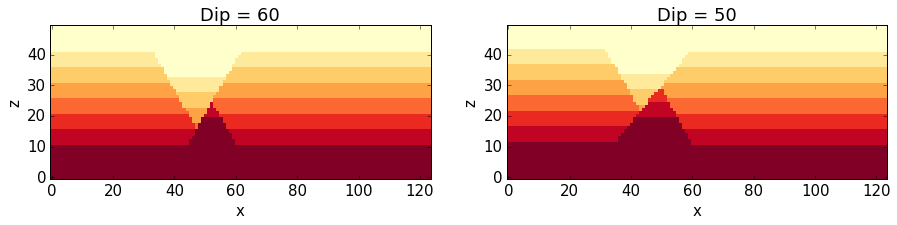
\includegraphics{3-Events_13_0.png}
\caption{png}\end{figure}


\section{Changing the order of geological events}
\label{notebooks/3-Events:changing-the-order-of-geological-events}
The geological history is parameterised as single events in a timeline.
Changing the order of events can be performed with two basic methods:
\begin{enumerate}
\item {} 
Swapping two events with a simple command

\item {} 
Adjusting the entire timeline with a complete remapping of events

\end{enumerate}

The first method is probably the most useful to test how a simple change
in the order of events will effect the final geological model. We will
use it here with our example to test how the model would change if the
timing of the faults is swapped.

The method to swap two geological events is defined on the level of the
history object:

\begin{Verbatim}[commandchars=\\\{\}]
\PYG{n}{H1} \PYG{o}{=} \PYG{n}{pynoddy}\PYG{o}{.}\PYG{n}{history}\PYG{o}{.}\PYG{n}{NoddyHistory}\PYG{p}{(}\PYG{n}{history\PYGZus{}ori}\PYG{p}{)}
\end{Verbatim}

\begin{Verbatim}[commandchars=\\\{\}]
\PYG{c}{\PYGZsh{} The names of the two fault events defined in the history file are:}
\PYG{k}{print} \PYG{n}{H1}\PYG{o}{.}\PYG{n}{events}\PYG{p}{[}\PYG{l+m+mi}{2}\PYG{p}{]}\PYG{o}{.}\PYG{n}{name}
\PYG{k}{print} \PYG{n}{H1}\PYG{o}{.}\PYG{n}{events}\PYG{p}{[}\PYG{l+m+mi}{3}\PYG{p}{]}\PYG{o}{.}\PYG{n}{name}
\end{Verbatim}

\begin{Verbatim}[commandchars=\\\{\}]
\PYG{n}{Fault2}
\PYG{n}{Fault1}
\end{Verbatim}

We now swap the position of two events in the kinematic history. For
this purpose, a high-level function can directly be used:

\begin{Verbatim}[commandchars=\\\{\}]
\PYG{c}{\PYGZsh{} Now: swap the events:}
\PYG{n}{H1}\PYG{o}{.}\PYG{n}{swap\PYGZus{}events}\PYG{p}{(}\PYG{l+m+mi}{2}\PYG{p}{,}\PYG{l+m+mi}{3}\PYG{p}{)}
\end{Verbatim}

\begin{Verbatim}[commandchars=\\\{\}]
\PYG{c}{\PYGZsh{} And let\PYGZsq{}s check if this is correctly relfected in the events order now:}
\PYG{k}{print} \PYG{n}{H1}\PYG{o}{.}\PYG{n}{events}\PYG{p}{[}\PYG{l+m+mi}{2}\PYG{p}{]}\PYG{o}{.}\PYG{n}{name}
\PYG{k}{print} \PYG{n}{H1}\PYG{o}{.}\PYG{n}{events}\PYG{p}{[}\PYG{l+m+mi}{3}\PYG{p}{]}\PYG{o}{.}\PYG{n}{name}
\end{Verbatim}

\begin{Verbatim}[commandchars=\\\{\}]
\PYG{n}{Fault1}
\PYG{n}{Fault2}
\end{Verbatim}

Now let's create a new history file and evaluate the effect of the
changed order in a cross section view:

\begin{Verbatim}[commandchars=\\\{\}]
\PYG{n}{new\PYGZus{}history} \PYG{o}{=} \PYG{l+s}{\PYGZdq{}}\PYG{l+s}{faults\PYGZus{}changed\PYGZus{}order.his}\PYG{l+s}{\PYGZdq{}}
\PYG{n}{new\PYGZus{}output} \PYG{o}{=} \PYG{l+s}{\PYGZdq{}}\PYG{l+s}{faults\PYGZus{}out}\PYG{l+s}{\PYGZdq{}}
\PYG{n}{H1}\PYG{o}{.}\PYG{n}{write\PYGZus{}history}\PYG{p}{(}\PYG{n}{new\PYGZus{}history}\PYG{p}{)}
\PYG{n}{pynoddy}\PYG{o}{.}\PYG{n}{compute\PYGZus{}model}\PYG{p}{(}\PYG{n}{new\PYGZus{}history}\PYG{p}{,} \PYG{n}{new\PYGZus{}output}\PYG{p}{)}
\end{Verbatim}

\begin{Verbatim}[commandchars=\\\{\}]
\PYG{l+s}{\PYGZsq{}}\PYG{l+s}{\PYGZsq{}}
\end{Verbatim}

\begin{Verbatim}[commandchars=\\\{\}]
\PYG{n+nb}{reload}\PYG{p}{(}\PYG{n}{pynoddy}\PYG{o}{.}\PYG{n}{output}\PYG{p}{)}
\PYG{c}{\PYGZsh{} Load and compare both models}
\PYG{n}{NO1} \PYG{o}{=} \PYG{n}{pynoddy}\PYG{o}{.}\PYG{n}{output}\PYG{o}{.}\PYG{n}{NoddyOutput}\PYG{p}{(}\PYG{n}{output\PYGZus{}name}\PYG{p}{)}
\PYG{n}{NO2} \PYG{o}{=} \PYG{n}{pynoddy}\PYG{o}{.}\PYG{n}{output}\PYG{o}{.}\PYG{n}{NoddyOutput}\PYG{p}{(}\PYG{n}{new\PYGZus{}output}\PYG{p}{)}
\PYG{c}{\PYGZsh{} create basic figure layout}
\PYG{n}{fig} \PYG{o}{=} \PYG{n}{plt}\PYG{o}{.}\PYG{n}{figure}\PYG{p}{(}\PYG{n}{figsize} \PYG{o}{=} \PYG{p}{(}\PYG{l+m+mi}{15}\PYG{p}{,}\PYG{l+m+mi}{5}\PYG{p}{)}\PYG{p}{)}
\PYG{n}{ax1} \PYG{o}{=} \PYG{n}{fig}\PYG{o}{.}\PYG{n}{add\PYGZus{}subplot}\PYG{p}{(}\PYG{l+m+mi}{121}\PYG{p}{)}
\PYG{n}{ax2} \PYG{o}{=} \PYG{n}{fig}\PYG{o}{.}\PYG{n}{add\PYGZus{}subplot}\PYG{p}{(}\PYG{l+m+mi}{122}\PYG{p}{)}
\PYG{n}{NO1}\PYG{o}{.}\PYG{n}{plot\PYGZus{}section}\PYG{p}{(}\PYG{l+s}{\PYGZsq{}}\PYG{l+s}{y}\PYG{l+s}{\PYGZsq{}}\PYG{p}{,} \PYG{n}{ax} \PYG{o}{=} \PYG{n}{ax1}\PYG{p}{,} \PYG{n}{colorbar}\PYG{o}{=}\PYG{n+nb+bp}{False}\PYG{p}{,} \PYG{n}{title}\PYG{o}{=}\PYG{l+s}{\PYGZdq{}}\PYG{l+s}{Model 1}\PYG{l+s}{\PYGZdq{}}\PYG{p}{)}
\PYG{n}{NO2}\PYG{o}{.}\PYG{n}{plot\PYGZus{}section}\PYG{p}{(}\PYG{l+s}{\PYGZsq{}}\PYG{l+s}{y}\PYG{l+s}{\PYGZsq{}}\PYG{p}{,} \PYG{n}{ax} \PYG{o}{=} \PYG{n}{ax2}\PYG{p}{,} \PYG{n}{colorbar}\PYG{o}{=}\PYG{n+nb+bp}{False}\PYG{p}{,} \PYG{n}{title}\PYG{o}{=}\PYG{l+s}{\PYGZdq{}}\PYG{l+s}{Model 2}\PYG{l+s}{\PYGZdq{}}\PYG{p}{)}

\PYG{n}{plt}\PYG{o}{.}\PYG{n}{show}\PYG{p}{(}\PYG{p}{)}
\end{Verbatim}
\begin{figure}[htbp]
\centering
\capstart

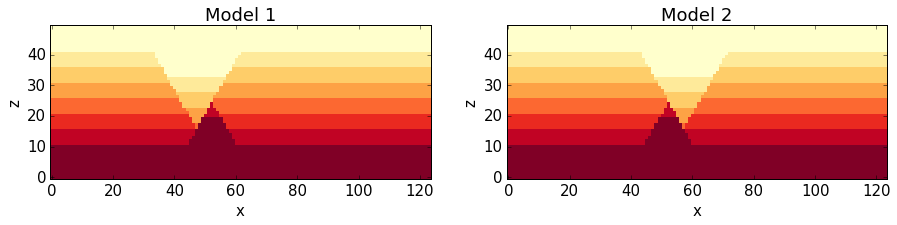
\includegraphics{3-Events_22_0.png}
\caption{png}\end{figure}


\section{Determining the stratigraphic difference between two models}
\label{notebooks/3-Events:determining-the-stratigraphic-difference-between-two-models}
Just as another quick example of a possible application of pynoddy to
evaluate aspects that are not simply possible with, for example, the GUI
version of Noddy itself. In the last example with the changed order of
the faults, we might be interested to determine where in space this
change had an effect. We can test this quite simply using the
\code{NoddyOutput} objects.

The geology data is stored in the \code{NoddyOutput.block} attribute. To
evaluate the difference between two models, we can therefore simply
compute:

\begin{Verbatim}[commandchars=\\\{\}]
\PYG{n}{diff} \PYG{o}{=} \PYG{p}{(}\PYG{n}{NO2}\PYG{o}{.}\PYG{n}{block} \PYG{o}{\PYGZhy{}} \PYG{n}{NO1}\PYG{o}{.}\PYG{n}{block}\PYG{p}{)}
\end{Verbatim}

And create a simple visualisation of the difference in a slice plot
with:

\begin{Verbatim}[commandchars=\\\{\}]
\PYG{n}{fig} \PYG{o}{=} \PYG{n}{plt}\PYG{o}{.}\PYG{n}{figure}\PYG{p}{(}\PYG{n}{figsize} \PYG{o}{=} \PYG{p}{(}\PYG{l+m+mi}{5}\PYG{p}{,}\PYG{l+m+mi}{3}\PYG{p}{)}\PYG{p}{)}
\PYG{n}{ax} \PYG{o}{=} \PYG{n}{fig}\PYG{o}{.}\PYG{n}{add\PYGZus{}subplot}\PYG{p}{(}\PYG{l+m+mi}{111}\PYG{p}{)}
\PYG{n}{ax}\PYG{o}{.}\PYG{n}{imshow}\PYG{p}{(}\PYG{n}{diff}\PYG{p}{[}\PYG{p}{:}\PYG{p}{,}\PYG{l+m+mi}{10}\PYG{p}{,}\PYG{p}{:}\PYG{p}{]}\PYG{o}{.}\PYG{n}{transpose}\PYG{p}{(}\PYG{p}{)}\PYG{p}{,} \PYG{n}{interpolation}\PYG{o}{=}\PYG{l+s}{\PYGZsq{}}\PYG{l+s}{nearest}\PYG{l+s}{\PYGZsq{}}\PYG{p}{,}
          \PYG{n}{cmap} \PYG{o}{=} \PYG{l+s}{\PYGZdq{}}\PYG{l+s}{RdBu}\PYG{l+s}{\PYGZdq{}}\PYG{p}{,} \PYG{n}{origin} \PYG{o}{=} \PYG{l+s}{\PYGZsq{}}\PYG{l+s}{lower left}\PYG{l+s}{\PYGZsq{}}\PYG{p}{)}
\end{Verbatim}

\begin{Verbatim}[commandchars=\\\{\}]
\PYGZlt{}matplotlib.image.AxesImage at 0x10cf3be10\PYGZgt{}
\end{Verbatim}
\begin{figure}[htbp]
\centering
\capstart

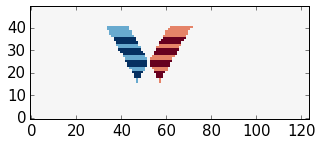
\includegraphics{3-Events_26_1.png}
\caption{png}\end{figure}

(Adding a meaningful title and axis labels to the plot is left to the
reader as simple excercise :-) Future versions of pynoddy might provide
an automatic implementation for this step...)

Again, we may want to visualise results in 3-D. We can use the
\code{export\_to\_vtk}-function as before, but now assing the data array to
be exported as the calulcated differnce field:

\begin{Verbatim}[commandchars=\\\{\}]
\PYG{n}{NO1}\PYG{o}{.}\PYG{n}{export\PYGZus{}to\PYGZus{}vtk}\PYG{p}{(}\PYG{n}{vtk\PYGZus{}filename} \PYG{o}{=} \PYG{l+s}{\PYGZdq{}}\PYG{l+s}{model\PYGZus{}diff}\PYG{l+s}{\PYGZdq{}}\PYG{p}{,} \PYG{n}{data} \PYG{o}{=} \PYG{n}{diff}\PYG{p}{)}
\end{Verbatim}

A 3-D view of the difference plot is presented below.
\begin{figure}[htbp]
\centering
\capstart

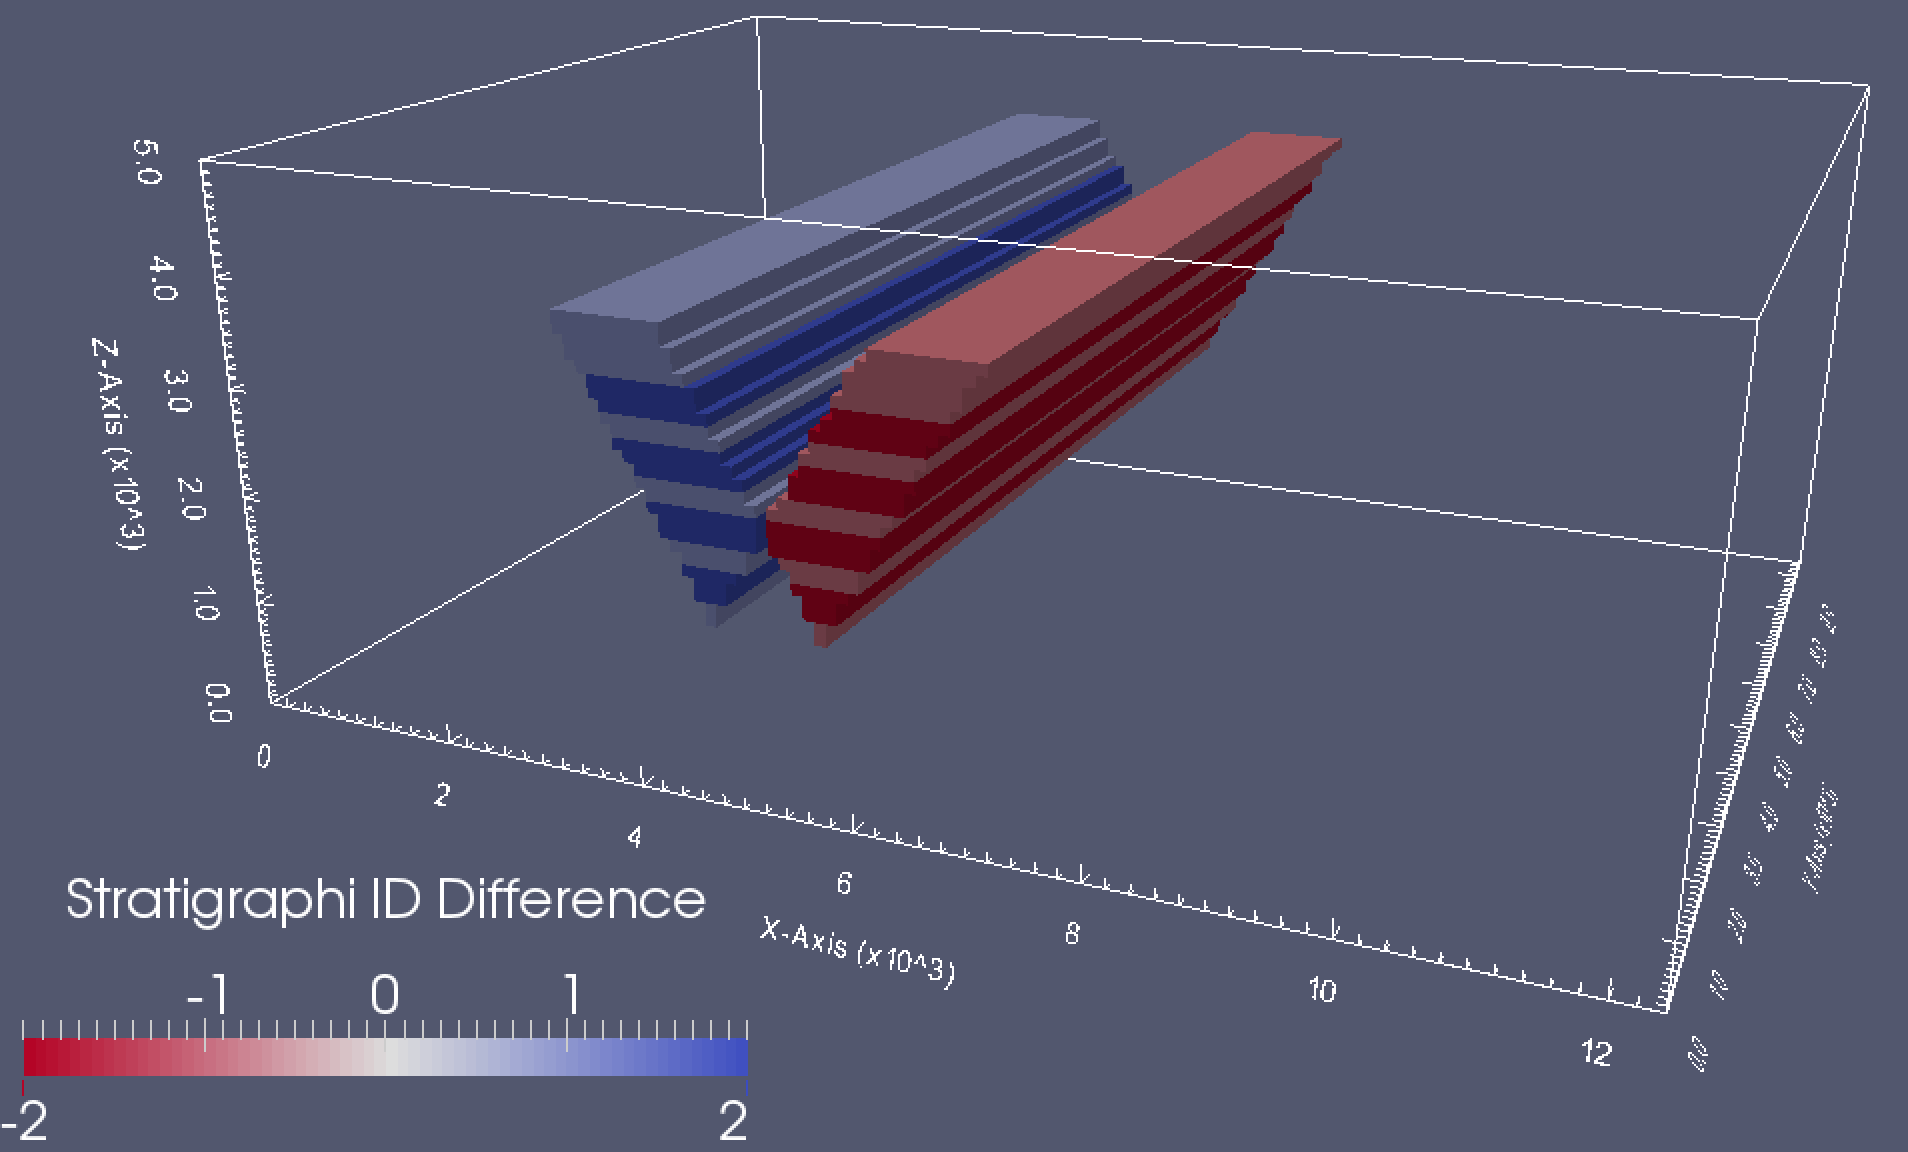
\includegraphics{diff_3d_3.png}
\caption{3-D visualisation of stratigraphic id difference}\end{figure}


\chapter{Creating a model from scratch}
\label{notebooks/4-Create-model:creating-a-model-from-scratch}\label{notebooks/4-Create-model::doc}
We describe here how to generate a simple history file for computation
with Noddy using the functionality of pynoddy. If possible, it is
advisable to generate the history files with the Windows GUI for Noddy
as this method provides, to date, a simpler and more complete interface
to the entire functionality.

For completeness, pynoddy contains the functionality to generate simple
models, for example to automate the model construction process, or to
enable the model construction for users who are not running Windows.
Some simple examlpes are shown in the following.

\begin{Verbatim}[commandchars=\\\{\}]
\PYG{k+kn}{from} \PYG{n+nn}{matplotlib} \PYG{k+kn}{import} \PYG{n}{rc\PYGZus{}params}
\end{Verbatim}

\begin{Verbatim}[commandchars=\\\{\}]
\PYG{k+kn}{from} \PYG{n+nn}{IPython.core.display} \PYG{k+kn}{import} \PYG{n}{HTML}
\PYG{n}{css\PYGZus{}file} \PYG{o}{=} \PYG{l+s}{\PYGZsq{}}\PYG{l+s}{pynoddy.css}\PYG{l+s}{\PYGZsq{}}
\PYG{n}{HTML}\PYG{p}{(}\PYG{n+nb}{open}\PYG{p}{(}\PYG{n}{css\PYGZus{}file}\PYG{p}{,} \PYG{l+s}{\PYGZdq{}}\PYG{l+s}{r}\PYG{l+s}{\PYGZdq{}}\PYG{p}{)}\PYG{o}{.}\PYG{n}{read}\PYG{p}{(}\PYG{p}{)}\PYG{p}{)}
\end{Verbatim}

\begin{Verbatim}[commandchars=\\\{\}]
\PYG{k+kn}{import} \PYG{n+nn}{sys}\PYG{o}{,} \PYG{n+nn}{os}
\PYG{k+kn}{import} \PYG{n+nn}{matplotlib.pyplot} \PYG{k+kn}{as} \PYG{n+nn}{plt}
\PYG{c}{\PYGZsh{} adjust some settings for matplotlib}
\PYG{k+kn}{from} \PYG{n+nn}{matplotlib} \PYG{k+kn}{import} \PYG{n}{rcParams}
\PYG{c}{\PYGZsh{} print rcParams}
\PYG{n}{rcParams}\PYG{p}{[}\PYG{l+s}{\PYGZsq{}}\PYG{l+s}{font.size}\PYG{l+s}{\PYGZsq{}}\PYG{p}{]} \PYG{o}{=} \PYG{l+m+mi}{15}
\PYG{c}{\PYGZsh{} determine path of repository to set paths corretly below}
\PYG{n}{repo\PYGZus{}path} \PYG{o}{=} \PYG{n}{os}\PYG{o}{.}\PYG{n}{path}\PYG{o}{.}\PYG{n}{realpath}\PYG{p}{(}\PYG{l+s}{\PYGZsq{}}\PYG{l+s}{../..}\PYG{l+s}{\PYGZsq{}}\PYG{p}{)}
\PYG{k+kn}{import} \PYG{n+nn}{pynoddy.history}
\end{Verbatim}

\begin{Verbatim}[commandchars=\\\{\}]
\PYGZpc{}matplotlib inline
\end{Verbatim}

\begin{Verbatim}[commandchars=\\\{\}]
\PYG{n}{rcParams}\PYG{o}{.}\PYG{n}{update}\PYG{p}{(}\PYG{p}{\PYGZob{}}\PYG{l+s}{\PYGZsq{}}\PYG{l+s}{font.size}\PYG{l+s}{\PYGZsq{}}\PYG{p}{:} \PYG{l+m+mi}{20}\PYG{p}{\PYGZcb{}}\PYG{p}{)}
\end{Verbatim}


\section{Defining a stratigraphy}
\label{notebooks/4-Create-model:defining-a-stratigraphy}
We start with the definition of a (base) stratigraphy for the model.

\begin{Verbatim}[commandchars=\\\{\}]
\PYG{c}{\PYGZsh{} Combined: model generation and output vis to test:}
\PYG{n}{history} \PYG{o}{=} \PYG{l+s}{\PYGZdq{}}\PYG{l+s}{simple\PYGZus{}model.his}\PYG{l+s}{\PYGZdq{}}
\PYG{n}{output\PYGZus{}name} \PYG{o}{=} \PYG{l+s}{\PYGZdq{}}\PYG{l+s}{simple\PYGZus{}out}\PYG{l+s}{\PYGZdq{}}
\PYG{n+nb}{reload}\PYG{p}{(}\PYG{n}{pynoddy}\PYG{o}{.}\PYG{n}{history}\PYG{p}{)}
\PYG{n+nb}{reload}\PYG{p}{(}\PYG{n}{pynoddy}\PYG{o}{.}\PYG{n}{events}\PYG{p}{)}

\PYG{c}{\PYGZsh{} create pynoddy object}
\PYG{n}{nm} \PYG{o}{=} \PYG{n}{pynoddy}\PYG{o}{.}\PYG{n}{history}\PYG{o}{.}\PYG{n}{NoddyHistory}\PYG{p}{(}\PYG{p}{)}
\PYG{c}{\PYGZsh{} add stratigraphy}
\PYG{n}{strati\PYGZus{}options} \PYG{o}{=} \PYG{p}{\PYGZob{}}\PYG{l+s}{\PYGZsq{}}\PYG{l+s}{num\PYGZus{}layers}\PYG{l+s}{\PYGZsq{}} \PYG{p}{:} \PYG{l+m+mi}{8}\PYG{p}{,}
                  \PYG{l+s}{\PYGZsq{}}\PYG{l+s}{layer\PYGZus{}names}\PYG{l+s}{\PYGZsq{}} \PYG{p}{:} \PYG{p}{[}\PYG{l+s}{\PYGZsq{}}\PYG{l+s}{layer 1}\PYG{l+s}{\PYGZsq{}}\PYG{p}{,} \PYG{l+s}{\PYGZsq{}}\PYG{l+s}{layer 2}\PYG{l+s}{\PYGZsq{}}\PYG{p}{,} \PYG{l+s}{\PYGZsq{}}\PYG{l+s}{layer 3}\PYG{l+s}{\PYGZsq{}}\PYG{p}{,}
                                   \PYG{l+s}{\PYGZsq{}}\PYG{l+s}{layer 4}\PYG{l+s}{\PYGZsq{}}\PYG{p}{,} \PYG{l+s}{\PYGZsq{}}\PYG{l+s}{layer 5}\PYG{l+s}{\PYGZsq{}}\PYG{p}{,} \PYG{l+s}{\PYGZsq{}}\PYG{l+s}{layer 6}\PYG{l+s}{\PYGZsq{}}\PYG{p}{,}
                                   \PYG{l+s}{\PYGZsq{}}\PYG{l+s}{layer 7}\PYG{l+s}{\PYGZsq{}}\PYG{p}{,} \PYG{l+s}{\PYGZsq{}}\PYG{l+s}{layer 8}\PYG{l+s}{\PYGZsq{}}\PYG{p}{]}\PYG{p}{,}
                  \PYG{l+s}{\PYGZsq{}}\PYG{l+s}{layer\PYGZus{}thickness}\PYG{l+s}{\PYGZsq{}} \PYG{p}{:} \PYG{p}{[}\PYG{l+m+mi}{1500}\PYG{p}{,} \PYG{l+m+mi}{500}\PYG{p}{,} \PYG{l+m+mi}{500}\PYG{p}{,} \PYG{l+m+mi}{500}\PYG{p}{,} \PYG{l+m+mi}{500}\PYG{p}{,} \PYG{l+m+mi}{500}\PYG{p}{,} \PYG{l+m+mi}{500}\PYG{p}{,} \PYG{l+m+mi}{500}\PYG{p}{]}\PYG{p}{\PYGZcb{}}
\PYG{n}{nm}\PYG{o}{.}\PYG{n}{add\PYGZus{}event}\PYG{p}{(}\PYG{l+s}{\PYGZsq{}}\PYG{l+s}{stratigraphy}\PYG{l+s}{\PYGZsq{}}\PYG{p}{,} \PYG{n}{strati\PYGZus{}options} \PYG{p}{)}

\PYG{n}{nm}\PYG{o}{.}\PYG{n}{write\PYGZus{}history}\PYG{p}{(}\PYG{n}{history}\PYG{p}{)}
\end{Verbatim}

\begin{Verbatim}[commandchars=\\\{\}]
\PYG{c}{\PYGZsh{} Compute the model}
\PYG{n+nb}{reload}\PYG{p}{(}\PYG{n}{pynoddy}\PYG{p}{)}
\PYG{n}{pynoddy}\PYG{o}{.}\PYG{n}{compute\PYGZus{}model}\PYG{p}{(}\PYG{n}{history}\PYG{p}{,} \PYG{n}{output\PYGZus{}name}\PYG{p}{)}
\end{Verbatim}

\begin{Verbatim}[commandchars=\\\{\}]
\PYG{l+s}{\PYGZsq{}}\PYG{l+s}{\PYGZsq{}}
\end{Verbatim}

\begin{Verbatim}[commandchars=\\\{\}]
\PYG{c}{\PYGZsh{} Plot output}
\PYG{k+kn}{import} \PYG{n+nn}{pynoddy.output}
\PYG{n+nb}{reload}\PYG{p}{(}\PYG{n}{pynoddy}\PYG{o}{.}\PYG{n}{output}\PYG{p}{)}
\PYG{n}{nout} \PYG{o}{=} \PYG{n}{pynoddy}\PYG{o}{.}\PYG{n}{output}\PYG{o}{.}\PYG{n}{NoddyOutput}\PYG{p}{(}\PYG{n}{output\PYGZus{}name}\PYG{p}{)}
\PYG{n}{nout}\PYG{o}{.}\PYG{n}{plot\PYGZus{}section}\PYG{p}{(}\PYG{l+s}{\PYGZsq{}}\PYG{l+s}{y}\PYG{l+s}{\PYGZsq{}}\PYG{p}{,} \PYG{n}{layer\PYGZus{}labels} \PYG{o}{=} \PYG{n}{strati\PYGZus{}options}\PYG{p}{[}\PYG{l+s}{\PYGZsq{}}\PYG{l+s}{layer\PYGZus{}names}\PYG{l+s}{\PYGZsq{}}\PYG{p}{]}\PYG{p}{[}\PYG{p}{:}\PYG{p}{:}\PYG{o}{\PYGZhy{}}\PYG{l+m+mi}{1}\PYG{p}{]}\PYG{p}{,}
                  \PYG{n}{colorbar} \PYG{o}{=} \PYG{n+nb+bp}{True}\PYG{p}{,} \PYG{n}{title}\PYG{o}{=}\PYG{l+s}{\PYGZdq{}}\PYG{l+s}{\PYGZdq{}}\PYG{p}{,}
                  \PYG{n}{savefig} \PYG{o}{=} \PYG{n+nb+bp}{False}\PYG{p}{,} \PYG{n}{fig\PYGZus{}filename} \PYG{o}{=} \PYG{l+s}{\PYGZdq{}}\PYG{l+s}{ex01\PYGZus{}strati.eps}\PYG{l+s}{\PYGZdq{}}\PYG{p}{)}
\end{Verbatim}
\begin{figure}[htbp]
\centering
\capstart

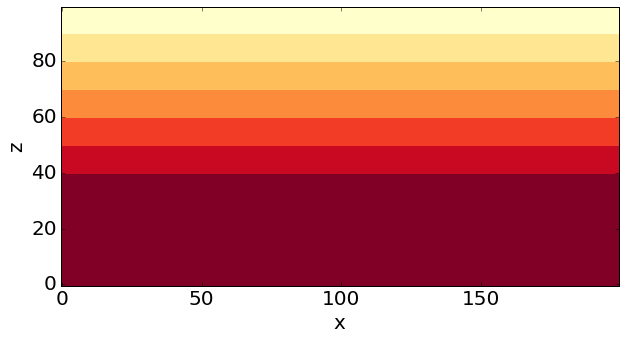
\includegraphics{4-Create-model_9_0.png}
\caption{png}\end{figure}


\section{Add a fault event}
\label{notebooks/4-Create-model:add-a-fault-event}
As a next step, let's now add the faults to the model.

\begin{Verbatim}[commandchars=\\\{\}]
\PYG{n+nb}{reload}\PYG{p}{(}\PYG{n}{pynoddy}\PYG{o}{.}\PYG{n}{history}\PYG{p}{)}
\PYG{n+nb}{reload}\PYG{p}{(}\PYG{n}{pynoddy}\PYG{o}{.}\PYG{n}{events}\PYG{p}{)}
\PYG{n}{nm} \PYG{o}{=} \PYG{n}{pynoddy}\PYG{o}{.}\PYG{n}{history}\PYG{o}{.}\PYG{n}{NoddyHistory}\PYG{p}{(}\PYG{p}{)}
\PYG{c}{\PYGZsh{} add stratigraphy}
\PYG{n}{strati\PYGZus{}options} \PYG{o}{=} \PYG{p}{\PYGZob{}}\PYG{l+s}{\PYGZsq{}}\PYG{l+s}{num\PYGZus{}layers}\PYG{l+s}{\PYGZsq{}} \PYG{p}{:} \PYG{l+m+mi}{8}\PYG{p}{,}
                  \PYG{l+s}{\PYGZsq{}}\PYG{l+s}{layer\PYGZus{}names}\PYG{l+s}{\PYGZsq{}} \PYG{p}{:} \PYG{p}{[}\PYG{l+s}{\PYGZsq{}}\PYG{l+s}{layer 1}\PYG{l+s}{\PYGZsq{}}\PYG{p}{,} \PYG{l+s}{\PYGZsq{}}\PYG{l+s}{layer 2}\PYG{l+s}{\PYGZsq{}}\PYG{p}{,} \PYG{l+s}{\PYGZsq{}}\PYG{l+s}{layer 3}\PYG{l+s}{\PYGZsq{}}\PYG{p}{,} \PYG{l+s}{\PYGZsq{}}\PYG{l+s}{layer 4}\PYG{l+s}{\PYGZsq{}}\PYG{p}{,} \PYG{l+s}{\PYGZsq{}}\PYG{l+s}{layer 5}\PYG{l+s}{\PYGZsq{}}\PYG{p}{,} \PYG{l+s}{\PYGZsq{}}\PYG{l+s}{layer 6}\PYG{l+s}{\PYGZsq{}}\PYG{p}{,} \PYG{l+s}{\PYGZsq{}}\PYG{l+s}{layer 7}\PYG{l+s}{\PYGZsq{}}\PYG{p}{,} \PYG{l+s}{\PYGZsq{}}\PYG{l+s}{layer 8}\PYG{l+s}{\PYGZsq{}}\PYG{p}{]}\PYG{p}{,}
                  \PYG{l+s}{\PYGZsq{}}\PYG{l+s}{layer\PYGZus{}thickness}\PYG{l+s}{\PYGZsq{}} \PYG{p}{:} \PYG{p}{[}\PYG{l+m+mi}{1500}\PYG{p}{,} \PYG{l+m+mi}{500}\PYG{p}{,} \PYG{l+m+mi}{500}\PYG{p}{,} \PYG{l+m+mi}{500}\PYG{p}{,} \PYG{l+m+mi}{500}\PYG{p}{,} \PYG{l+m+mi}{500}\PYG{p}{,} \PYG{l+m+mi}{500}\PYG{p}{,} \PYG{l+m+mi}{500}\PYG{p}{]}\PYG{p}{\PYGZcb{}}
\PYG{n}{nm}\PYG{o}{.}\PYG{n}{add\PYGZus{}event}\PYG{p}{(}\PYG{l+s}{\PYGZsq{}}\PYG{l+s}{stratigraphy}\PYG{l+s}{\PYGZsq{}}\PYG{p}{,} \PYG{n}{strati\PYGZus{}options} \PYG{p}{)}




\PYG{c}{\PYGZsh{} The following options define the fault geometry:}
\PYG{n}{fault\PYGZus{}options} \PYG{o}{=} \PYG{p}{\PYGZob{}}\PYG{l+s}{\PYGZsq{}}\PYG{l+s}{name}\PYG{l+s}{\PYGZsq{}} \PYG{p}{:} \PYG{l+s}{\PYGZsq{}}\PYG{l+s}{Fault\PYGZus{}E}\PYG{l+s}{\PYGZsq{}}\PYG{p}{,}
                 \PYG{l+s}{\PYGZsq{}}\PYG{l+s}{pos}\PYG{l+s}{\PYGZsq{}} \PYG{p}{:} \PYG{p}{(}\PYG{l+m+mi}{6000}\PYG{p}{,} \PYG{l+m+mi}{0}\PYG{p}{,} \PYG{l+m+mi}{5000}\PYG{p}{)}\PYG{p}{,}
                 \PYG{l+s}{\PYGZsq{}}\PYG{l+s}{dip\PYGZus{}dir}\PYG{l+s}{\PYGZsq{}} \PYG{p}{:} \PYG{l+m+mi}{270}\PYG{p}{,}
                 \PYG{l+s}{\PYGZsq{}}\PYG{l+s}{dip}\PYG{l+s}{\PYGZsq{}} \PYG{p}{:} \PYG{l+m+mi}{60}\PYG{p}{,}
                 \PYG{l+s}{\PYGZsq{}}\PYG{l+s}{slip}\PYG{l+s}{\PYGZsq{}} \PYG{p}{:} \PYG{l+m+mi}{1000}\PYG{p}{\PYGZcb{}}

\PYG{n}{nm}\PYG{o}{.}\PYG{n}{add\PYGZus{}event}\PYG{p}{(}\PYG{l+s}{\PYGZsq{}}\PYG{l+s}{fault}\PYG{l+s}{\PYGZsq{}}\PYG{p}{,} \PYG{n}{fault\PYGZus{}options}\PYG{p}{)}
\end{Verbatim}

\begin{Verbatim}[commandchars=\\\{\}]
\PYG{n}{nm}\PYG{o}{.}\PYG{n}{events}
\end{Verbatim}

\begin{Verbatim}[commandchars=\\\{\}]
\PYGZob{}1: \PYGZlt{}pynoddy.events.Stratigraphy at 0x1073fc590\PYGZgt{},
 2: \PYGZlt{}pynoddy.events.Fault at 0x107565fd0\PYGZgt{}\PYGZcb{}
\end{Verbatim}

\begin{Verbatim}[commandchars=\\\{\}]
\PYG{n}{nm}\PYG{o}{.}\PYG{n}{write\PYGZus{}history}\PYG{p}{(}\PYG{n}{history}\PYG{p}{)}
\end{Verbatim}

\begin{Verbatim}[commandchars=\\\{\}]
\PYG{c}{\PYGZsh{} Compute the model}
\PYG{n}{pynoddy}\PYG{o}{.}\PYG{n}{compute\PYGZus{}model}\PYG{p}{(}\PYG{n}{history}\PYG{p}{,} \PYG{n}{output\PYGZus{}name}\PYG{p}{)}
\end{Verbatim}

\begin{Verbatim}[commandchars=\\\{\}]
\PYG{l+s}{\PYGZsq{}}\PYG{l+s}{\PYGZsq{}}
\end{Verbatim}

\begin{Verbatim}[commandchars=\\\{\}]
\PYG{c}{\PYGZsh{} Plot output}
\PYG{n+nb}{reload}\PYG{p}{(}\PYG{n}{pynoddy}\PYG{o}{.}\PYG{n}{output}\PYG{p}{)}
\PYG{n}{nout} \PYG{o}{=} \PYG{n}{pynoddy}\PYG{o}{.}\PYG{n}{output}\PYG{o}{.}\PYG{n}{NoddyOutput}\PYG{p}{(}\PYG{n}{output\PYGZus{}name}\PYG{p}{)}
\PYG{n}{nout}\PYG{o}{.}\PYG{n}{plot\PYGZus{}section}\PYG{p}{(}\PYG{l+s}{\PYGZsq{}}\PYG{l+s}{y}\PYG{l+s}{\PYGZsq{}}\PYG{p}{,} \PYG{n}{layer\PYGZus{}labels} \PYG{o}{=} \PYG{n}{strati\PYGZus{}options}\PYG{p}{[}\PYG{l+s}{\PYGZsq{}}\PYG{l+s}{layer\PYGZus{}names}\PYG{l+s}{\PYGZsq{}}\PYG{p}{]}\PYG{p}{[}\PYG{p}{:}\PYG{p}{:}\PYG{o}{\PYGZhy{}}\PYG{l+m+mi}{1}\PYG{p}{]}\PYG{p}{,}
                  \PYG{n}{colorbar} \PYG{o}{=} \PYG{n+nb+bp}{True}\PYG{p}{,} \PYG{n}{title} \PYG{o}{=} \PYG{l+s}{\PYGZdq{}}\PYG{l+s}{\PYGZdq{}}\PYG{p}{,}
                  \PYG{n}{savefig} \PYG{o}{=} \PYG{n+nb+bp}{False}\PYG{p}{,} \PYG{n}{fig\PYGZus{}filename} \PYG{o}{=} \PYG{l+s}{\PYGZdq{}}\PYG{l+s}{ex01\PYGZus{}fault\PYGZus{}E.eps}\PYG{l+s}{\PYGZdq{}}\PYG{p}{)}
\end{Verbatim}
\begin{figure}[htbp]
\centering
\capstart

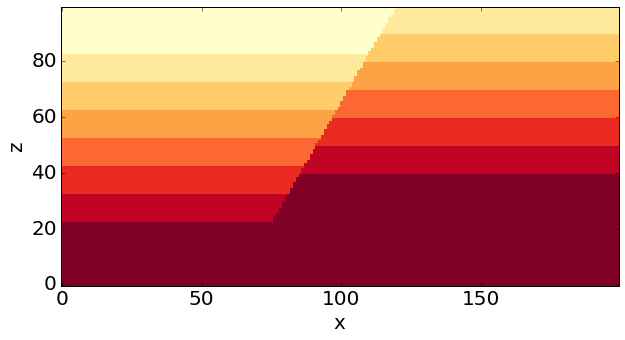
\includegraphics{4-Create-model_15_0.png}
\caption{png}\end{figure}

\begin{Verbatim}[commandchars=\\\{\}]
\PYG{c}{\PYGZsh{} The following options define the fault geometry:}
\PYG{n}{fault\PYGZus{}options} \PYG{o}{=} \PYG{p}{\PYGZob{}}\PYG{l+s}{\PYGZsq{}}\PYG{l+s}{name}\PYG{l+s}{\PYGZsq{}} \PYG{p}{:} \PYG{l+s}{\PYGZsq{}}\PYG{l+s}{Fault\PYGZus{}1}\PYG{l+s}{\PYGZsq{}}\PYG{p}{,}
                 \PYG{l+s}{\PYGZsq{}}\PYG{l+s}{pos}\PYG{l+s}{\PYGZsq{}} \PYG{p}{:} \PYG{p}{(}\PYG{l+m+mi}{5500}\PYG{p}{,} \PYG{l+m+mi}{3500}\PYG{p}{,} \PYG{l+m+mi}{0}\PYG{p}{)}\PYG{p}{,}
                 \PYG{l+s}{\PYGZsq{}}\PYG{l+s}{dip\PYGZus{}dir}\PYG{l+s}{\PYGZsq{}} \PYG{p}{:} \PYG{l+m+mi}{270}\PYG{p}{,}
                 \PYG{l+s}{\PYGZsq{}}\PYG{l+s}{dip}\PYG{l+s}{\PYGZsq{}} \PYG{p}{:} \PYG{l+m+mi}{60}\PYG{p}{,}
                 \PYG{l+s}{\PYGZsq{}}\PYG{l+s}{slip}\PYG{l+s}{\PYGZsq{}} \PYG{p}{:} \PYG{l+m+mi}{1000}\PYG{p}{\PYGZcb{}}

\PYG{n}{nm}\PYG{o}{.}\PYG{n}{add\PYGZus{}event}\PYG{p}{(}\PYG{l+s}{\PYGZsq{}}\PYG{l+s}{fault}\PYG{l+s}{\PYGZsq{}}\PYG{p}{,} \PYG{n}{fault\PYGZus{}options}\PYG{p}{)}
\end{Verbatim}

\begin{Verbatim}[commandchars=\\\{\}]
\PYG{n}{nm}\PYG{o}{.}\PYG{n}{write\PYGZus{}history}\PYG{p}{(}\PYG{n}{history}\PYG{p}{)}
\end{Verbatim}

\begin{Verbatim}[commandchars=\\\{\}]
\PYG{c}{\PYGZsh{} Compute the model}
\PYG{n}{pynoddy}\PYG{o}{.}\PYG{n}{compute\PYGZus{}model}\PYG{p}{(}\PYG{n}{history}\PYG{p}{,} \PYG{n}{output\PYGZus{}name}\PYG{p}{)}
\end{Verbatim}

\begin{Verbatim}[commandchars=\\\{\}]
\PYG{l+s}{\PYGZsq{}}\PYG{l+s}{\PYGZsq{}}
\end{Verbatim}

\begin{Verbatim}[commandchars=\\\{\}]
\PYG{c}{\PYGZsh{} Plot output}
\PYG{n+nb}{reload}\PYG{p}{(}\PYG{n}{pynoddy}\PYG{o}{.}\PYG{n}{output}\PYG{p}{)}
\PYG{n}{nout} \PYG{o}{=} \PYG{n}{pynoddy}\PYG{o}{.}\PYG{n}{output}\PYG{o}{.}\PYG{n}{NoddyOutput}\PYG{p}{(}\PYG{n}{output\PYGZus{}name}\PYG{p}{)}
\PYG{n}{nout}\PYG{o}{.}\PYG{n}{plot\PYGZus{}section}\PYG{p}{(}\PYG{l+s}{\PYGZsq{}}\PYG{l+s}{y}\PYG{l+s}{\PYGZsq{}}\PYG{p}{,} \PYG{n}{layer\PYGZus{}labels} \PYG{o}{=} \PYG{n}{strati\PYGZus{}options}\PYG{p}{[}\PYG{l+s}{\PYGZsq{}}\PYG{l+s}{layer\PYGZus{}names}\PYG{l+s}{\PYGZsq{}}\PYG{p}{]}\PYG{p}{[}\PYG{p}{:}\PYG{p}{:}\PYG{o}{\PYGZhy{}}\PYG{l+m+mi}{1}\PYG{p}{]}\PYG{p}{,} \PYG{n}{colorbar} \PYG{o}{=} \PYG{n+nb+bp}{True}\PYG{p}{)}
\end{Verbatim}
\begin{figure}[htbp]
\centering
\capstart

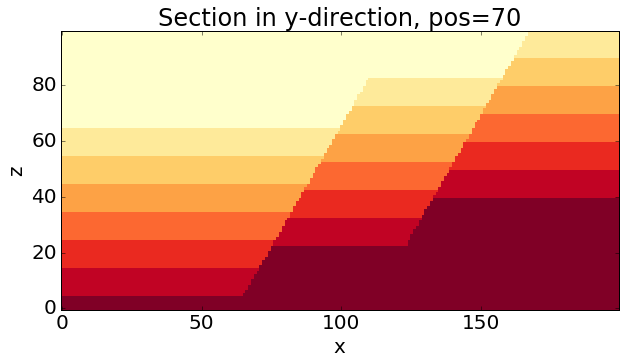
\includegraphics{4-Create-model_19_0.png}
\caption{png}\end{figure}

\begin{Verbatim}[commandchars=\\\{\}]
\PYG{n}{nm1} \PYG{o}{=} \PYG{n}{pynoddy}\PYG{o}{.}\PYG{n}{history}\PYG{o}{.}\PYG{n}{NoddyHistory}\PYG{p}{(}\PYG{n}{history}\PYG{p}{)}
\end{Verbatim}

\begin{Verbatim}[commandchars=\\\{\}]
\PYG{n}{nm1}\PYG{o}{.}\PYG{n}{get\PYGZus{}extent}\PYG{p}{(}\PYG{p}{)}
\end{Verbatim}

\begin{Verbatim}[commandchars=\\\{\}]
\PYG{p}{(}\PYG{l+m+mf}{10000.0}\PYG{p}{,} \PYG{l+m+mf}{7000.0}\PYG{p}{,} \PYG{l+m+mf}{5000.0}\PYG{p}{)}
\end{Verbatim}


\section{Complete Model Set-up}
\label{notebooks/4-Create-model:complete-model-set-up}
And here now, combining all the previous steps, the entire model set-up
with base stratigraphy and two faults:

\begin{Verbatim}[commandchars=\\\{\}]
\PYG{n+nb}{reload}\PYG{p}{(}\PYG{n}{pynoddy}\PYG{o}{.}\PYG{n}{history}\PYG{p}{)}
\PYG{n+nb}{reload}\PYG{p}{(}\PYG{n}{pynoddy}\PYG{o}{.}\PYG{n}{events}\PYG{p}{)}
\PYG{n}{nm} \PYG{o}{=} \PYG{n}{pynoddy}\PYG{o}{.}\PYG{n}{history}\PYG{o}{.}\PYG{n}{NoddyHistory}\PYG{p}{(}\PYG{p}{)}
\PYG{c}{\PYGZsh{} add stratigraphy}
\PYG{n}{strati\PYGZus{}options} \PYG{o}{=} \PYG{p}{\PYGZob{}}\PYG{l+s}{\PYGZsq{}}\PYG{l+s}{num\PYGZus{}layers}\PYG{l+s}{\PYGZsq{}} \PYG{p}{:} \PYG{l+m+mi}{8}\PYG{p}{,}
                  \PYG{l+s}{\PYGZsq{}}\PYG{l+s}{layer\PYGZus{}names}\PYG{l+s}{\PYGZsq{}} \PYG{p}{:} \PYG{p}{[}\PYG{l+s}{\PYGZsq{}}\PYG{l+s}{layer 1}\PYG{l+s}{\PYGZsq{}}\PYG{p}{,} \PYG{l+s}{\PYGZsq{}}\PYG{l+s}{layer 2}\PYG{l+s}{\PYGZsq{}}\PYG{p}{,} \PYG{l+s}{\PYGZsq{}}\PYG{l+s}{layer 3}\PYG{l+s}{\PYGZsq{}}\PYG{p}{,}
                                   \PYG{l+s}{\PYGZsq{}}\PYG{l+s}{layer 4}\PYG{l+s}{\PYGZsq{}}\PYG{p}{,} \PYG{l+s}{\PYGZsq{}}\PYG{l+s}{layer 5}\PYG{l+s}{\PYGZsq{}}\PYG{p}{,} \PYG{l+s}{\PYGZsq{}}\PYG{l+s}{layer 6}\PYG{l+s}{\PYGZsq{}}\PYG{p}{,}
                                   \PYG{l+s}{\PYGZsq{}}\PYG{l+s}{layer 7}\PYG{l+s}{\PYGZsq{}}\PYG{p}{,} \PYG{l+s}{\PYGZsq{}}\PYG{l+s}{layer 8}\PYG{l+s}{\PYGZsq{}}\PYG{p}{]}\PYG{p}{,}
                  \PYG{l+s}{\PYGZsq{}}\PYG{l+s}{layer\PYGZus{}thickness}\PYG{l+s}{\PYGZsq{}} \PYG{p}{:} \PYG{p}{[}\PYG{l+m+mi}{1500}\PYG{p}{,} \PYG{l+m+mi}{500}\PYG{p}{,} \PYG{l+m+mi}{500}\PYG{p}{,} \PYG{l+m+mi}{500}\PYG{p}{,} \PYG{l+m+mi}{500}\PYG{p}{,}
                                       \PYG{l+m+mi}{500}\PYG{p}{,} \PYG{l+m+mi}{500}\PYG{p}{,} \PYG{l+m+mi}{500}\PYG{p}{]}\PYG{p}{\PYGZcb{}}
\PYG{n}{nm}\PYG{o}{.}\PYG{n}{add\PYGZus{}event}\PYG{p}{(}\PYG{l+s}{\PYGZsq{}}\PYG{l+s}{stratigraphy}\PYG{l+s}{\PYGZsq{}}\PYG{p}{,} \PYG{n}{strati\PYGZus{}options} \PYG{p}{)}

\PYG{c}{\PYGZsh{} The following options define the fault geometry:}
\PYG{n}{fault\PYGZus{}options} \PYG{o}{=} \PYG{p}{\PYGZob{}}\PYG{l+s}{\PYGZsq{}}\PYG{l+s}{name}\PYG{l+s}{\PYGZsq{}} \PYG{p}{:} \PYG{l+s}{\PYGZsq{}}\PYG{l+s}{Fault\PYGZus{}W}\PYG{l+s}{\PYGZsq{}}\PYG{p}{,}
                 \PYG{l+s}{\PYGZsq{}}\PYG{l+s}{pos}\PYG{l+s}{\PYGZsq{}} \PYG{p}{:} \PYG{p}{(}\PYG{l+m+mi}{4000}\PYG{p}{,} \PYG{l+m+mi}{3500}\PYG{p}{,} \PYG{l+m+mi}{5000}\PYG{p}{)}\PYG{p}{,}
                 \PYG{l+s}{\PYGZsq{}}\PYG{l+s}{dip\PYGZus{}dir}\PYG{l+s}{\PYGZsq{}} \PYG{p}{:} \PYG{l+m+mi}{90}\PYG{p}{,}
                 \PYG{l+s}{\PYGZsq{}}\PYG{l+s}{dip}\PYG{l+s}{\PYGZsq{}} \PYG{p}{:} \PYG{l+m+mi}{60}\PYG{p}{,}
                 \PYG{l+s}{\PYGZsq{}}\PYG{l+s}{slip}\PYG{l+s}{\PYGZsq{}} \PYG{p}{:} \PYG{l+m+mi}{1000}\PYG{p}{\PYGZcb{}}

\PYG{n}{nm}\PYG{o}{.}\PYG{n}{add\PYGZus{}event}\PYG{p}{(}\PYG{l+s}{\PYGZsq{}}\PYG{l+s}{fault}\PYG{l+s}{\PYGZsq{}}\PYG{p}{,} \PYG{n}{fault\PYGZus{}options}\PYG{p}{)}
\PYG{c}{\PYGZsh{} The following options define the fault geometry:}
\PYG{n}{fault\PYGZus{}options} \PYG{o}{=} \PYG{p}{\PYGZob{}}\PYG{l+s}{\PYGZsq{}}\PYG{l+s}{name}\PYG{l+s}{\PYGZsq{}} \PYG{p}{:} \PYG{l+s}{\PYGZsq{}}\PYG{l+s}{Fault\PYGZus{}E}\PYG{l+s}{\PYGZsq{}}\PYG{p}{,}
                 \PYG{l+s}{\PYGZsq{}}\PYG{l+s}{pos}\PYG{l+s}{\PYGZsq{}} \PYG{p}{:} \PYG{p}{(}\PYG{l+m+mi}{6000}\PYG{p}{,} \PYG{l+m+mi}{3500}\PYG{p}{,} \PYG{l+m+mi}{5000}\PYG{p}{)}\PYG{p}{,}
                 \PYG{l+s}{\PYGZsq{}}\PYG{l+s}{dip\PYGZus{}dir}\PYG{l+s}{\PYGZsq{}} \PYG{p}{:} \PYG{l+m+mi}{270}\PYG{p}{,}
                 \PYG{l+s}{\PYGZsq{}}\PYG{l+s}{dip}\PYG{l+s}{\PYGZsq{}} \PYG{p}{:} \PYG{l+m+mi}{60}\PYG{p}{,}
                 \PYG{l+s}{\PYGZsq{}}\PYG{l+s}{slip}\PYG{l+s}{\PYGZsq{}} \PYG{p}{:} \PYG{l+m+mi}{1000}\PYG{p}{\PYGZcb{}}

\PYG{n}{nm}\PYG{o}{.}\PYG{n}{add\PYGZus{}event}\PYG{p}{(}\PYG{l+s}{\PYGZsq{}}\PYG{l+s}{fault}\PYG{l+s}{\PYGZsq{}}\PYG{p}{,} \PYG{n}{fault\PYGZus{}options}\PYG{p}{)}
\PYG{n}{nm}\PYG{o}{.}\PYG{n}{write\PYGZus{}history}\PYG{p}{(}\PYG{n}{history}\PYG{p}{)}
\end{Verbatim}

\begin{Verbatim}[commandchars=\\\{\}]
\PYG{c}{\PYGZsh{} Change cube size}
\PYG{n}{nm1} \PYG{o}{=} \PYG{n}{pynoddy}\PYG{o}{.}\PYG{n}{history}\PYG{o}{.}\PYG{n}{NoddyHistory}\PYG{p}{(}\PYG{n}{history}\PYG{p}{)}
\PYG{n}{nm1}\PYG{o}{.}\PYG{n}{change\PYGZus{}cube\PYGZus{}size}\PYG{p}{(}\PYG{l+m+mi}{50}\PYG{p}{)}
\PYG{n}{nm1}\PYG{o}{.}\PYG{n}{write\PYGZus{}history}\PYG{p}{(}\PYG{n}{history}\PYG{p}{)}
\end{Verbatim}

\begin{Verbatim}[commandchars=\\\{\}]
\PYG{c}{\PYGZsh{} Compute the model}
\PYG{n}{pynoddy}\PYG{o}{.}\PYG{n}{compute\PYGZus{}model}\PYG{p}{(}\PYG{n}{history}\PYG{p}{,} \PYG{n}{output\PYGZus{}name}\PYG{p}{)}
\end{Verbatim}

\begin{Verbatim}[commandchars=\\\{\}]
\PYG{l+s}{\PYGZsq{}}\PYG{l+s}{\PYGZsq{}}
\end{Verbatim}

\begin{Verbatim}[commandchars=\\\{\}]
\PYG{c}{\PYGZsh{} Plot output}
\PYG{n+nb}{reload}\PYG{p}{(}\PYG{n}{pynoddy}\PYG{o}{.}\PYG{n}{output}\PYG{p}{)}
\PYG{n}{nout} \PYG{o}{=} \PYG{n}{pynoddy}\PYG{o}{.}\PYG{n}{output}\PYG{o}{.}\PYG{n}{NoddyOutput}\PYG{p}{(}\PYG{n}{output\PYGZus{}name}\PYG{p}{)}
\PYG{n}{nout}\PYG{o}{.}\PYG{n}{plot\PYGZus{}section}\PYG{p}{(}\PYG{l+s}{\PYGZsq{}}\PYG{l+s}{y}\PYG{l+s}{\PYGZsq{}}\PYG{p}{,} \PYG{n}{layer\PYGZus{}labels} \PYG{o}{=} \PYG{n}{strati\PYGZus{}options}\PYG{p}{[}\PYG{l+s}{\PYGZsq{}}\PYG{l+s}{layer\PYGZus{}names}\PYG{l+s}{\PYGZsq{}}\PYG{p}{]}\PYG{p}{[}\PYG{p}{:}\PYG{p}{:}\PYG{o}{\PYGZhy{}}\PYG{l+m+mi}{1}\PYG{p}{]}\PYG{p}{,}
                  \PYG{n}{colorbar} \PYG{o}{=} \PYG{n+nb+bp}{True}\PYG{p}{,} \PYG{n}{title}\PYG{o}{=}\PYG{l+s}{\PYGZdq{}}\PYG{l+s}{\PYGZdq{}}\PYG{p}{,}
                  \PYG{n}{savefig} \PYG{o}{=} \PYG{n+nb+bp}{True}\PYG{p}{,} \PYG{n}{fig\PYGZus{}filename} \PYG{o}{=} \PYG{l+s}{\PYGZdq{}}\PYG{l+s}{ex01\PYGZus{}faults\PYGZus{}combined.eps}\PYG{l+s}{\PYGZdq{}}\PYG{p}{,}
                  \PYG{n}{cmap} \PYG{o}{=} \PYG{l+s}{\PYGZsq{}}\PYG{l+s}{YlOrRd}\PYG{l+s}{\PYGZsq{}}\PYG{p}{)} \PYG{c}{\PYGZsh{} note: YlOrRd colourmap should be suitable for colorblindness!}
\end{Verbatim}
\begin{figure}[htbp]
\centering
\capstart

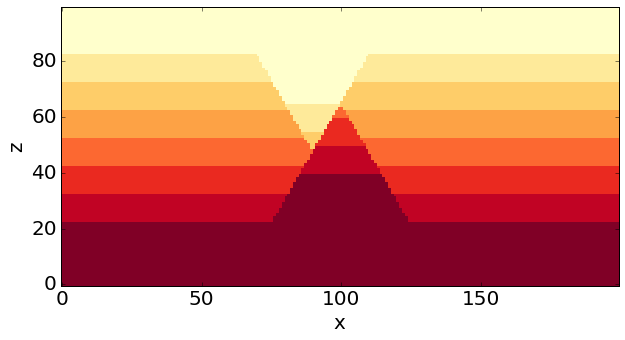
\includegraphics{4-Create-model_26_0.png}
\caption{png}\end{figure}


\chapter{Read and Visualise Geophysical Potential-Fields}
\label{notebooks/5-Geophysical-Potential-Fields::doc}\label{notebooks/5-Geophysical-Potential-Fields:read-and-visualise-geophysical-potential-fields}
Geophysical potential fields (gravity and magnetics) can be calculated
directly from the generated kinematic model. A wide range of options
also exists to consider effects of geological events on the relevant
rock properties. We will here use pynoddy to simply and quickly test the
effect of changing geological structures on the calculated geophysical
response.

\begin{Verbatim}[commandchars=\\\{\}]
\PYGZpc{}matplotlib inline
\end{Verbatim}

\begin{Verbatim}[commandchars=\\\{\}]
\PYG{k+kn}{import} \PYG{n+nn}{sys}\PYG{o}{,} \PYG{n+nn}{os}
\PYG{k+kn}{import} \PYG{n+nn}{matplotlib.pyplot} \PYG{k+kn}{as} \PYG{n+nn}{plt}
\PYG{c}{\PYGZsh{} adjust some settings for matplotlib}
\PYG{k+kn}{from} \PYG{n+nn}{matplotlib} \PYG{k+kn}{import} \PYG{n}{rcParams}
\PYG{c}{\PYGZsh{} print rcParams}
\PYG{n}{rcParams}\PYG{p}{[}\PYG{l+s}{\PYGZsq{}}\PYG{l+s}{font.size}\PYG{l+s}{\PYGZsq{}}\PYG{p}{]} \PYG{o}{=} \PYG{l+m+mi}{15}
\PYG{c}{\PYGZsh{} determine path of repository to set paths corretly below}
\PYG{n}{repo\PYGZus{}path} \PYG{o}{=} \PYG{n}{os}\PYG{o}{.}\PYG{n}{path}\PYG{o}{.}\PYG{n}{realpath}\PYG{p}{(}\PYG{l+s}{\PYGZsq{}}\PYG{l+s}{../..}\PYG{l+s}{\PYGZsq{}}\PYG{p}{)}
\PYG{k+kn}{import} \PYG{n+nn}{pynoddy}
\end{Verbatim}

\begin{Verbatim}[commandchars=\\\{\}]
\PYG{k+kn}{import} \PYG{n+nn}{matplotlib.pyplot} \PYG{k+kn}{as} \PYG{n+nn}{plt}
\PYG{k+kn}{import} \PYG{n+nn}{numpy} \PYG{k+kn}{as} \PYG{n+nn}{np}
\end{Verbatim}

\begin{Verbatim}[commandchars=\\\{\}]
\PYG{k+kn}{from} \PYG{n+nn}{IPython.core.display} \PYG{k+kn}{import} \PYG{n}{HTML}
\PYG{n}{css\PYGZus{}file} \PYG{o}{=} \PYG{l+s}{\PYGZsq{}}\PYG{l+s}{pynoddy.css}\PYG{l+s}{\PYGZsq{}}
\PYG{n}{HTML}\PYG{p}{(}\PYG{n+nb}{open}\PYG{p}{(}\PYG{n}{css\PYGZus{}file}\PYG{p}{,} \PYG{l+s}{\PYGZdq{}}\PYG{l+s}{r}\PYG{l+s}{\PYGZdq{}}\PYG{p}{)}\PYG{o}{.}\PYG{n}{read}\PYG{p}{(}\PYG{p}{)}\PYG{p}{)}
\end{Verbatim}


\section{Read history file from Virtual Explorer}
\label{notebooks/5-Geophysical-Potential-Fields:read-history-file-from-virtual-explorer}
Many Noddy models are available on the site of the Virtual Explorer in
the Structural Geophysics Atlas. We will download and use one of these
models here as the base model.

We start with the history file of a ``Fold and Thrust Belt'' setting
stored on:

\code{http://virtualexplorer.com.au/special/noddyatlas/ch3/ch3\_5/his/nfold\_thrust.his}

The file can directly be downloaded and opened with pynoddy:

\begin{Verbatim}[commandchars=\\\{\}]
\PYG{k+kn}{import} \PYG{n+nn}{pynoddy.history}
\PYG{n+nb}{reload}\PYG{p}{(}\PYG{n}{pynoddy}\PYG{o}{.}\PYG{n}{history}\PYG{p}{)}

\PYG{n}{his} \PYG{o}{=} \PYG{n}{pynoddy}\PYG{o}{.}\PYG{n}{history}\PYG{o}{.}\PYG{n}{NoddyHistory}\PYG{p}{(}\PYG{n}{url} \PYG{o}{=} \PYGZbs{}
            \PYG{l+s}{\PYGZdq{}}\PYG{l+s}{http://tectonique.net/asg/ch3/ch3\PYGZus{}5/his/fold\PYGZus{}thrust.his}\PYG{l+s}{\PYGZdq{}}\PYG{p}{)}

\PYG{n}{his}\PYG{o}{.}\PYG{n}{determine\PYGZus{}model\PYGZus{}stratigraphy}\PYG{p}{(}\PYG{p}{)}
\end{Verbatim}

\begin{Verbatim}[commandchars=\\\{\}]
\PYG{n}{his}\PYG{o}{.}\PYG{n}{change\PYGZus{}cube\PYGZus{}size}\PYG{p}{(}\PYG{l+m+mi}{50}\PYG{p}{)}
\end{Verbatim}

\begin{Verbatim}[commandchars=\\\{\}]
\PYG{c}{\PYGZsh{} Save to (local) file to compute and visualise model}
\PYG{n}{history\PYGZus{}name} \PYG{o}{=} \PYG{l+s}{\PYGZdq{}}\PYG{l+s}{fold\PYGZus{}thrust.his}\PYG{l+s}{\PYGZdq{}}
\PYG{n}{his}\PYG{o}{.}\PYG{n}{write\PYGZus{}history}\PYG{p}{(}\PYG{n}{history\PYGZus{}name}\PYG{p}{)}
\PYG{c}{\PYGZsh{} his = pynoddy.history.NoddyHistory(history\PYGZus{}name)}
\end{Verbatim}

\begin{Verbatim}[commandchars=\\\{\}]
\PYG{n}{output} \PYG{o}{=} \PYG{l+s}{\PYGZdq{}}\PYG{l+s}{fold\PYGZus{}thrust\PYGZus{}out}\PYG{l+s}{\PYGZdq{}}
\PYG{n}{pynoddy}\PYG{o}{.}\PYG{n}{compute\PYGZus{}model}\PYG{p}{(}\PYG{n}{history\PYGZus{}name}\PYG{p}{,} \PYG{n}{output}\PYG{p}{)}
\end{Verbatim}

\begin{Verbatim}[commandchars=\\\{\}]
\PYG{l+s}{\PYGZsq{}}\PYG{l+s}{\PYGZsq{}}
\end{Verbatim}

\begin{Verbatim}[commandchars=\\\{\}]
\PYG{k+kn}{import} \PYG{n+nn}{pynoddy.output}
\PYG{c}{\PYGZsh{} load and visualise model}
\PYG{n}{h\PYGZus{}out} \PYG{o}{=} \PYG{n}{pynoddy}\PYG{o}{.}\PYG{n}{output}\PYG{o}{.}\PYG{n}{NoddyOutput}\PYG{p}{(}\PYG{n}{output}\PYG{p}{)}
\end{Verbatim}

\begin{Verbatim}[commandchars=\\\{\}]
\PYG{c}{\PYGZsh{} his.determine\PYGZus{}model\PYGZus{}stratigraphy()}
\PYG{n}{h\PYGZus{}out}\PYG{o}{.}\PYG{n}{plot\PYGZus{}section}\PYG{p}{(}\PYG{l+s}{\PYGZsq{}}\PYG{l+s}{x}\PYG{l+s}{\PYGZsq{}}\PYG{p}{,}
                   \PYG{n}{layer\PYGZus{}labels} \PYG{o}{=} \PYG{n}{his}\PYG{o}{.}\PYG{n}{model\PYGZus{}stratigraphy}\PYG{p}{,}
                   \PYG{n}{colorbar\PYGZus{}orientation} \PYG{o}{=} \PYG{l+s}{\PYGZsq{}}\PYG{l+s}{horizontal}\PYG{l+s}{\PYGZsq{}}\PYG{p}{,}
                   \PYG{n}{colorbar}\PYG{o}{=}\PYG{n+nb+bp}{False}\PYG{p}{,}
                   \PYG{n}{title} \PYG{o}{=} \PYG{l+s}{\PYGZsq{}}\PYG{l+s}{\PYGZsq{}}\PYG{p}{,}
\PYG{c}{\PYGZsh{}                   savefig=True, fig\PYGZus{}filename = \PYGZsq{}fold\PYGZus{}thrust\PYGZus{}NS\PYGZus{}section.eps\PYGZsq{},}
                   \PYG{n}{cmap} \PYG{o}{=} \PYG{l+s}{\PYGZsq{}}\PYG{l+s}{YlOrRd}\PYG{l+s}{\PYGZsq{}}\PYG{p}{)}
\end{Verbatim}
\begin{figure}[htbp]
\centering
\capstart

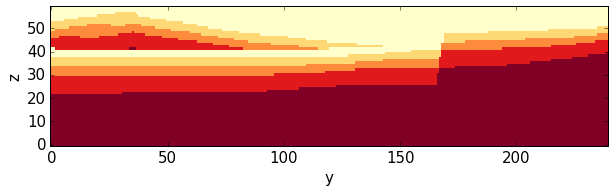
\includegraphics{5-Geophysical-Potential-Fields_11_0.png}
\caption{png}\end{figure}

\begin{Verbatim}[commandchars=\\\{\}]
\PYG{n}{h\PYGZus{}out}\PYG{o}{.}\PYG{n}{plot\PYGZus{}section}\PYG{p}{(}\PYG{l+s}{\PYGZsq{}}\PYG{l+s}{y}\PYG{l+s}{\PYGZsq{}}\PYG{p}{,} \PYG{n}{layer\PYGZus{}labels} \PYG{o}{=} \PYG{n}{his}\PYG{o}{.}\PYG{n}{model\PYGZus{}stratigraphy}\PYG{p}{,}
                   \PYG{n}{colorbar\PYGZus{}orientation} \PYG{o}{=} \PYG{l+s}{\PYGZsq{}}\PYG{l+s}{horizontal}\PYG{l+s}{\PYGZsq{}}\PYG{p}{,} \PYG{n}{title} \PYG{o}{=} \PYG{l+s}{\PYGZsq{}}\PYG{l+s}{\PYGZsq{}}\PYG{p}{,} \PYG{n}{cmap} \PYG{o}{=} \PYG{l+s}{\PYGZsq{}}\PYG{l+s}{YlOrRd}\PYG{l+s}{\PYGZsq{}}\PYG{p}{,}
\PYG{c}{\PYGZsh{}                   savefig=True, fig\PYGZus{}filename = \PYGZsq{}fold\PYGZus{}thrust\PYGZus{}EW\PYGZus{}section.eps\PYGZsq{},}
                   \PYG{n}{ve}\PYG{o}{=}\PYG{l+m+mf}{1.5}\PYG{p}{)}
\end{Verbatim}
\begin{figure}[htbp]
\centering
\capstart

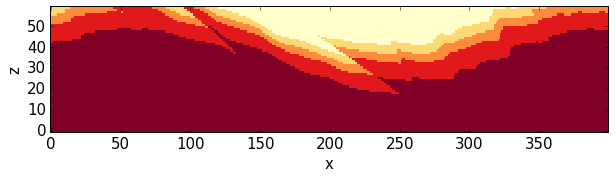
\includegraphics{5-Geophysical-Potential-Fields_12_0.png}
\caption{png}\end{figure}

\begin{Verbatim}[commandchars=\\\{\}]
\PYG{n}{h\PYGZus{}out}\PYG{o}{.}\PYG{n}{export\PYGZus{}to\PYGZus{}vtk}\PYG{p}{(}\PYG{n}{vtk\PYGZus{}filename} \PYG{o}{=} \PYG{l+s}{\PYGZdq{}}\PYG{l+s}{fold\PYGZus{}thrust}\PYG{l+s}{\PYGZdq{}}\PYG{p}{)}
\end{Verbatim}


\section{Visualise calculated geophysical fields}
\label{notebooks/5-Geophysical-Potential-Fields:visualise-calculated-geophysical-fields}
The first step is to recompute the model with the generation of the
geophysical responses

\begin{Verbatim}[commandchars=\\\{\}]
\PYG{n}{pynoddy}\PYG{o}{.}\PYG{n}{compute\PYGZus{}model}\PYG{p}{(}\PYG{n}{history\PYGZus{}name}\PYG{p}{,} \PYG{n}{output}\PYG{p}{,} \PYG{n}{sim\PYGZus{}type} \PYG{o}{=} \PYG{l+s}{\PYGZsq{}}\PYG{l+s}{GEOPHYSICS}\PYG{l+s}{\PYGZsq{}}\PYG{p}{)}
\end{Verbatim}

\begin{Verbatim}[commandchars=\\\{\}]
\PYG{l+s}{\PYGZsq{}}\PYG{l+s}{\PYGZsq{}}
\end{Verbatim}

We now get two files for the caluclated fields: `.grv' for gravity, and
`.mag' for the magnetic field. We can extract the information of these
files for visualisation and further processing in python:

\begin{Verbatim}[commandchars=\\\{\}]
\PYG{n+nb}{reload}\PYG{p}{(}\PYG{n}{pynoddy}\PYG{o}{.}\PYG{n}{output}\PYG{p}{)}
\PYG{n}{geophys} \PYG{o}{=} \PYG{n}{pynoddy}\PYG{o}{.}\PYG{n}{output}\PYG{o}{.}\PYG{n}{NoddyGeophysics}\PYG{p}{(}\PYG{n}{output}\PYG{p}{)}
\end{Verbatim}

\begin{Verbatim}[commandchars=\\\{\}]
\PYG{n}{fig} \PYG{o}{=} \PYG{n}{plt}\PYG{o}{.}\PYG{n}{figure}\PYG{p}{(}\PYG{n}{figsize} \PYG{o}{=} \PYG{p}{(}\PYG{l+m+mi}{5}\PYG{p}{,}\PYG{l+m+mi}{5}\PYG{p}{)}\PYG{p}{)}
\PYG{n}{ax} \PYG{o}{=} \PYG{n}{fig}\PYG{o}{.}\PYG{n}{add\PYGZus{}subplot}\PYG{p}{(}\PYG{l+m+mi}{111}\PYG{p}{)}
\PYG{c}{\PYGZsh{} imshow(geophys.grv\PYGZus{}data, cmap = \PYGZsq{}jet\PYGZsq{})}
\PYG{c}{\PYGZsh{} define contour levels}
\PYG{n}{levels} \PYG{o}{=} \PYG{n}{np}\PYG{o}{.}\PYG{n}{arange}\PYG{p}{(}\PYG{l+m+mi}{322}\PYG{p}{,}\PYG{l+m+mi}{344}\PYG{p}{,}\PYG{l+m+mi}{1}\PYG{p}{)}
\PYG{n}{cf} \PYG{o}{=} \PYG{n}{ax}\PYG{o}{.}\PYG{n}{contourf}\PYG{p}{(}\PYG{n}{geophys}\PYG{o}{.}\PYG{n}{grv\PYGZus{}data}\PYG{p}{,} \PYG{n}{levels}\PYG{p}{,} \PYG{n}{cmap} \PYG{o}{=} \PYG{l+s}{\PYGZsq{}}\PYG{l+s}{gray}\PYG{l+s}{\PYGZsq{}}\PYG{p}{,} \PYG{n}{vmin} \PYG{o}{=} \PYG{l+m+mi}{324}\PYG{p}{,} \PYG{n}{vmax} \PYG{o}{=} \PYG{l+m+mi}{342}\PYG{p}{)}
\PYG{n}{cbar} \PYG{o}{=} \PYG{n}{plt}\PYG{o}{.}\PYG{n}{colorbar}\PYG{p}{(}\PYG{n}{cf}\PYG{p}{,} \PYG{n}{orientation} \PYG{o}{=} \PYG{l+s}{\PYGZsq{}}\PYG{l+s}{horizontal}\PYG{l+s}{\PYGZsq{}}\PYG{p}{)}
\PYG{c}{\PYGZsh{} print levels}
\end{Verbatim}
\begin{figure}[htbp]
\centering
\capstart

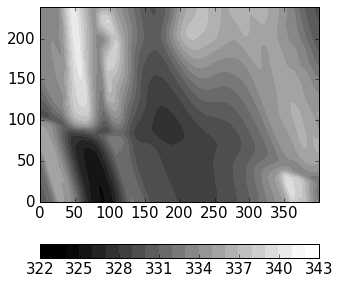
\includegraphics{5-Geophysical-Potential-Fields_18_0.png}
\caption{png}\end{figure}


\section{Change history and compare gravity}
\label{notebooks/5-Geophysical-Potential-Fields:change-history-and-compare-gravity}
As a next step, we will now change aspects of the geological history
(paramtereised in as parameters of the kinematic events) and calculate
the effect on the gravity. Then, we will compare the changed gravity
field to the original field.

Let's have a look at the properties of the defined faults in the
original model:

\begin{Verbatim}[commandchars=\\\{\}]
\PYG{k}{for} \PYG{n}{i} \PYG{o+ow}{in} \PYG{n+nb}{range}\PYG{p}{(}\PYG{l+m+mi}{4}\PYG{p}{)}\PYG{p}{:}
    \PYG{k}{print}\PYG{p}{(}\PYG{l+s}{\PYGZdq{}}\PYG{l+s+se}{\PYGZbs{}n}\PYG{l+s}{Event }\PYG{l+s+si}{\PYGZpc{}d}\PYG{l+s}{\PYGZdq{}} \PYG{o}{\PYGZpc{}} \PYG{p}{(}\PYG{n}{i}\PYG{o}{+}\PYG{l+m+mi}{2}\PYG{p}{)}\PYG{p}{)}
    \PYG{k}{print} \PYG{l+s}{\PYGZdq{}}\PYG{l+s}{Event type:}\PYG{l+s+se}{\PYGZbs{}t}\PYG{l+s}{\PYGZdq{}} \PYG{o}{+} \PYG{n}{his}\PYG{o}{.}\PYG{n}{events}\PYG{p}{[}\PYG{n}{i}\PYG{o}{+}\PYG{l+m+mi}{2}\PYG{p}{]}\PYG{o}{.}\PYG{n}{event\PYGZus{}type}
    \PYG{k}{print} \PYG{l+s}{\PYGZdq{}}\PYG{l+s}{Fault slip:}\PYG{l+s+se}{\PYGZbs{}t}\PYG{l+s+si}{\PYGZpc{}.1f}\PYG{l+s}{\PYGZdq{}} \PYG{o}{\PYGZpc{}} \PYG{n}{his}\PYG{o}{.}\PYG{n}{events}\PYG{p}{[}\PYG{n}{i}\PYG{o}{+}\PYG{l+m+mi}{2}\PYG{p}{]}\PYG{o}{.}\PYG{n}{properties}\PYG{p}{[}\PYG{l+s}{\PYGZsq{}}\PYG{l+s}{Slip}\PYG{l+s}{\PYGZsq{}}\PYG{p}{]}
    \PYG{k}{print} \PYG{l+s}{\PYGZdq{}}\PYG{l+s}{Fault dip:}\PYG{l+s+se}{\PYGZbs{}t}\PYG{l+s+si}{\PYGZpc{}.1f}\PYG{l+s}{\PYGZdq{}} \PYG{o}{\PYGZpc{}} \PYG{n}{his}\PYG{o}{.}\PYG{n}{events}\PYG{p}{[}\PYG{n}{i}\PYG{o}{+}\PYG{l+m+mi}{2}\PYG{p}{]}\PYG{o}{.}\PYG{n}{properties}\PYG{p}{[}\PYG{l+s}{\PYGZsq{}}\PYG{l+s}{Dip}\PYG{l+s}{\PYGZsq{}}\PYG{p}{]}
    \PYG{k}{print} \PYG{l+s}{\PYGZdq{}}\PYG{l+s}{Dip direction:}\PYG{l+s+se}{\PYGZbs{}t}\PYG{l+s+si}{\PYGZpc{}.1f}\PYG{l+s}{\PYGZdq{}} \PYG{o}{\PYGZpc{}} \PYG{n}{his}\PYG{o}{.}\PYG{n}{events}\PYG{p}{[}\PYG{n}{i}\PYG{o}{+}\PYG{l+m+mi}{2}\PYG{p}{]}\PYG{o}{.}\PYG{n}{properties}\PYG{p}{[}\PYG{l+s}{\PYGZsq{}}\PYG{l+s}{Dip Direction}\PYG{l+s}{\PYGZsq{}}\PYG{p}{]}
\end{Verbatim}

\begin{Verbatim}[commandchars=\\\{\}]
Event 2
Event type: FAULT
Fault slip: \PYGZhy{}5000.0
Fault dip:  0.0
Dip direction:  90.0

Event 3
Event type: FAULT
Fault slip: \PYGZhy{}3000.0
Fault dip:  0.0
Dip direction:  90.0

Event 4
Event type: FAULT
Fault slip: \PYGZhy{}3000.0
Fault dip:  0.0
Dip direction:  90.0

Event 5
Event type: FAULT
Fault slip: 12000.0
Fault dip:  80.0
Dip direction:  170.0
\end{Verbatim}

\begin{Verbatim}[commandchars=\\\{\}]
\PYG{n+nb}{reload}\PYG{p}{(}\PYG{n}{pynoddy}\PYG{o}{.}\PYG{n}{history}\PYG{p}{)}
\PYG{n+nb}{reload}\PYG{p}{(}\PYG{n}{pynoddy}\PYG{o}{.}\PYG{n}{events}\PYG{p}{)}
\PYG{n}{his2} \PYG{o}{=} \PYG{n}{pynoddy}\PYG{o}{.}\PYG{n}{history}\PYG{o}{.}\PYG{n}{NoddyHistory}\PYG{p}{(}\PYG{l+s}{\PYGZdq{}}\PYG{l+s}{fold\PYGZus{}thrust.his}\PYG{l+s}{\PYGZdq{}}\PYG{p}{)}

\PYG{k}{print} \PYG{n}{his2}\PYG{o}{.}\PYG{n}{events}\PYG{p}{[}\PYG{l+m+mi}{6}\PYG{p}{]}\PYG{o}{.}\PYG{n}{properties}
\end{Verbatim}

\begin{Verbatim}[commandchars=\\\{\}]
\PYG{p}{\PYGZob{}}\PYG{l+s}{\PYGZsq{}}\PYG{l+s}{Dip}\PYG{l+s}{\PYGZsq{}}\PYG{p}{:} \PYG{l+m+mf}{130.0}\PYG{p}{,} \PYG{l+s}{\PYGZsq{}}\PYG{l+s}{Cylindricity}\PYG{l+s}{\PYGZsq{}}\PYG{p}{:} \PYG{l+m+mf}{0.0}\PYG{p}{,} \PYG{l+s}{\PYGZsq{}}\PYG{l+s}{Wavelength}\PYG{l+s}{\PYGZsq{}}\PYG{p}{:} \PYG{l+m+mf}{12000.0}\PYG{p}{,} \PYG{l+s}{\PYGZsq{}}\PYG{l+s}{Amplitude}\PYG{l+s}{\PYGZsq{}}\PYG{p}{:} \PYG{l+m+mf}{1000.0}\PYG{p}{,} \PYG{l+s}{\PYGZsq{}}\PYG{l+s}{Pitch}\PYG{l+s}{\PYGZsq{}}\PYG{p}{:} \PYG{l+m+mf}{0.0}\PYG{p}{,} \PYG{l+s}{\PYGZsq{}}\PYG{l+s}{Y}\PYG{l+s}{\PYGZsq{}}\PYG{p}{:} \PYG{l+m+mf}{0.0}\PYG{p}{,} \PYG{l+s}{\PYGZsq{}}\PYG{l+s}{X}\PYG{l+s}{\PYGZsq{}}\PYG{p}{:} \PYG{l+m+mf}{0.0}\PYG{p}{,} \PYG{l+s}{\PYGZsq{}}\PYG{l+s}{Single Fold}\PYG{l+s}{\PYGZsq{}}\PYG{p}{:} \PYG{l+s}{\PYGZsq{}}\PYG{l+s}{FALSE}\PYG{l+s}{\PYGZsq{}}\PYG{p}{,} \PYG{l+s}{\PYGZsq{}}\PYG{l+s}{Z}\PYG{l+s}{\PYGZsq{}}\PYG{p}{:} \PYG{l+m+mf}{0.0}\PYG{p}{,} \PYG{l+s}{\PYGZsq{}}\PYG{l+s}{Type}\PYG{l+s}{\PYGZsq{}}\PYG{p}{:} \PYG{l+s}{\PYGZsq{}}\PYG{l+s}{Fourier}\PYG{l+s}{\PYGZsq{}}\PYG{p}{,} \PYG{l+s}{\PYGZsq{}}\PYG{l+s}{Dip Direction}\PYG{l+s}{\PYGZsq{}}\PYG{p}{:} \PYG{l+m+mf}{110.0}\PYG{p}{\PYGZcb{}}
\end{Verbatim}

As a simple test, we are changing the fault slip for all the faults and
simply add 1000 m to all defined slips. In order to not mess up the
original model, we are creating a copy of the history object first:

\begin{Verbatim}[commandchars=\\\{\}]
\PYG{k+kn}{import} \PYG{n+nn}{copy}
\PYG{n}{his} \PYG{o}{=} \PYG{n}{pynoddy}\PYG{o}{.}\PYG{n}{history}\PYG{o}{.}\PYG{n}{NoddyHistory}\PYG{p}{(}\PYG{n}{history\PYGZus{}name}\PYG{p}{)}
\PYG{n}{his}\PYG{o}{.}\PYG{n}{all\PYGZus{}events\PYGZus{}end} \PYG{o}{+}\PYG{o}{=} \PYG{l+m+mi}{1}
\PYG{n}{his\PYGZus{}changed} \PYG{o}{=} \PYG{n}{copy}\PYG{o}{.}\PYG{n}{deepcopy}\PYG{p}{(}\PYG{n}{his}\PYG{p}{)}

\PYG{c}{\PYGZsh{} change parameters of kinematic events}
\PYG{n}{slip\PYGZus{}change} \PYG{o}{=} \PYG{l+m+mf}{2000.}
\PYG{n}{wavelength\PYGZus{}change} \PYG{o}{=} \PYG{l+m+mf}{2000.}
\PYG{c}{\PYGZsh{} his\PYGZus{}changed.events[3].properties[\PYGZsq{}Slip\PYGZsq{}] += slip\PYGZus{}change}
\PYG{c}{\PYGZsh{} his\PYGZus{}changed.events[5].properties[\PYGZsq{}Slip\PYGZsq{}] += slip\PYGZus{}change}
\PYG{c}{\PYGZsh{} change fold wavelength}
\PYG{n}{his\PYGZus{}changed}\PYG{o}{.}\PYG{n}{events}\PYG{p}{[}\PYG{l+m+mi}{6}\PYG{p}{]}\PYG{o}{.}\PYG{n}{properties}\PYG{p}{[}\PYG{l+s}{\PYGZsq{}}\PYG{l+s}{Wavelength}\PYG{l+s}{\PYGZsq{}}\PYG{p}{]} \PYG{o}{+}\PYG{o}{=} \PYG{n}{wavelength\PYGZus{}change}
\PYG{n}{his\PYGZus{}changed}\PYG{o}{.}\PYG{n}{events}\PYG{p}{[}\PYG{l+m+mi}{6}\PYG{p}{]}\PYG{o}{.}\PYG{n}{properties}\PYG{p}{[}\PYG{l+s}{\PYGZsq{}}\PYG{l+s}{X}\PYG{l+s}{\PYGZsq{}}\PYG{p}{]} \PYG{o}{+}\PYG{o}{=} \PYG{n}{wavelength\PYGZus{}change}\PYG{o}{/}\PYG{l+m+mf}{2.}
\end{Verbatim}

We now write the adjusted history back to a new history file and then
calculate the updated gravity field:

\begin{Verbatim}[commandchars=\\\{\}]
\PYG{n}{his\PYGZus{}changed}\PYG{o}{.}\PYG{n}{write\PYGZus{}history}\PYG{p}{(}\PYG{l+s}{\PYGZsq{}}\PYG{l+s}{fold\PYGZus{}thrust\PYGZus{}changed.his}\PYG{l+s}{\PYGZsq{}}\PYG{p}{)}
\end{Verbatim}

\begin{Verbatim}[commandchars=\\\{\}]
\PYG{c}{\PYGZsh{} \PYGZpc{}\PYGZpc{}timeit}
\PYG{c}{\PYGZsh{} recompute block model}
\PYG{n}{pynoddy}\PYG{o}{.}\PYG{n}{compute\PYGZus{}model}\PYG{p}{(}\PYG{l+s}{\PYGZsq{}}\PYG{l+s}{fold\PYGZus{}thrust\PYGZus{}changed.his}\PYG{l+s}{\PYGZsq{}}\PYG{p}{,} \PYG{l+s}{\PYGZsq{}}\PYG{l+s}{fold\PYGZus{}thrust\PYGZus{}changed\PYGZus{}out}\PYG{l+s}{\PYGZsq{}}\PYG{p}{)}
\end{Verbatim}

\begin{Verbatim}[commandchars=\\\{\}]
\PYG{l+s}{\PYGZsq{}}\PYG{l+s}{\PYGZsq{}}
\end{Verbatim}

\begin{Verbatim}[commandchars=\\\{\}]
\PYG{c}{\PYGZsh{} \PYGZpc{}\PYGZpc{}timeit}
\PYG{c}{\PYGZsh{} recompute geophysical response}
\PYG{n}{pynoddy}\PYG{o}{.}\PYG{n}{compute\PYGZus{}model}\PYG{p}{(}\PYG{l+s}{\PYGZsq{}}\PYG{l+s}{fold\PYGZus{}thrust\PYGZus{}changed.his}\PYG{l+s}{\PYGZsq{}}\PYG{p}{,} \PYG{l+s}{\PYGZsq{}}\PYG{l+s}{fold\PYGZus{}thrust\PYGZus{}changed\PYGZus{}out}\PYG{l+s}{\PYGZsq{}}\PYG{p}{,}
                      \PYG{n}{sim\PYGZus{}type} \PYG{o}{=} \PYG{l+s}{\PYGZsq{}}\PYG{l+s}{GEOPHYSICS}\PYG{l+s}{\PYGZsq{}}\PYG{p}{)}
\end{Verbatim}

\begin{Verbatim}[commandchars=\\\{\}]
\PYG{l+s}{\PYGZsq{}}\PYG{l+s}{\PYGZsq{}}
\end{Verbatim}

\begin{Verbatim}[commandchars=\\\{\}]
\PYG{c}{\PYGZsh{} load changed block model}
\PYG{n}{geo\PYGZus{}changed} \PYG{o}{=} \PYG{n}{pynoddy}\PYG{o}{.}\PYG{n}{output}\PYG{o}{.}\PYG{n}{NoddyOutput}\PYG{p}{(}\PYG{l+s}{\PYGZsq{}}\PYG{l+s}{fold\PYGZus{}thrust\PYGZus{}changed\PYGZus{}out}\PYG{l+s}{\PYGZsq{}}\PYG{p}{)}
\PYG{c}{\PYGZsh{} load output and visualise geophysical field}
\PYG{n}{geophys\PYGZus{}changed} \PYG{o}{=} \PYG{n}{pynoddy}\PYG{o}{.}\PYG{n}{output}\PYG{o}{.}\PYG{n}{NoddyGeophysics}\PYG{p}{(}\PYG{l+s}{\PYGZsq{}}\PYG{l+s}{fold\PYGZus{}thrust\PYGZus{}changed\PYGZus{}out}\PYG{l+s}{\PYGZsq{}}\PYG{p}{)}
\end{Verbatim}

\begin{Verbatim}[commandchars=\\\{\}]
\PYG{n}{fig} \PYG{o}{=} \PYG{n}{plt}\PYG{o}{.}\PYG{n}{figure}\PYG{p}{(}\PYG{n}{figsize} \PYG{o}{=} \PYG{p}{(}\PYG{l+m+mi}{5}\PYG{p}{,}\PYG{l+m+mi}{5}\PYG{p}{)}\PYG{p}{)}
\PYG{n}{ax} \PYG{o}{=} \PYG{n}{fig}\PYG{o}{.}\PYG{n}{add\PYGZus{}subplot}\PYG{p}{(}\PYG{l+m+mi}{111}\PYG{p}{)}
\PYG{c}{\PYGZsh{} imshow(geophys\PYGZus{}changed.grv\PYGZus{}data, cmap = \PYGZsq{}jet\PYGZsq{})}
\PYG{n}{cf} \PYG{o}{=} \PYG{n}{ax}\PYG{o}{.}\PYG{n}{contourf}\PYG{p}{(}\PYG{n}{geophys\PYGZus{}changed}\PYG{o}{.}\PYG{n}{grv\PYGZus{}data}\PYG{p}{,} \PYG{n}{levels}\PYG{p}{,} \PYG{n}{cmap} \PYG{o}{=} \PYG{l+s}{\PYGZsq{}}\PYG{l+s}{gray}\PYG{l+s}{\PYGZsq{}}\PYG{p}{,} \PYG{n}{vmin} \PYG{o}{=} \PYG{l+m+mi}{324}\PYG{p}{,} \PYG{n}{vmax} \PYG{o}{=} \PYG{l+m+mi}{342}\PYG{p}{)}
\PYG{n}{cbar} \PYG{o}{=} \PYG{n}{plt}\PYG{o}{.}\PYG{n}{colorbar}\PYG{p}{(}\PYG{n}{cf}\PYG{p}{,} \PYG{n}{orientation} \PYG{o}{=} \PYG{l+s}{\PYGZsq{}}\PYG{l+s}{horizontal}\PYG{l+s}{\PYGZsq{}}\PYG{p}{)}
\end{Verbatim}
\begin{figure}[htbp]
\centering
\capstart

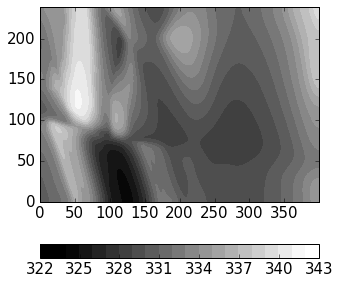
\includegraphics{5-Geophysical-Potential-Fields_30_0.png}
\caption{png}\end{figure}

\begin{Verbatim}[commandchars=\\\{\}]
\PYG{n}{fig} \PYG{o}{=} \PYG{n}{plt}\PYG{o}{.}\PYG{n}{figure}\PYG{p}{(}\PYG{n}{figsize} \PYG{o}{=} \PYG{p}{(}\PYG{l+m+mi}{5}\PYG{p}{,}\PYG{l+m+mi}{5}\PYG{p}{)}\PYG{p}{)}
\PYG{n}{ax} \PYG{o}{=} \PYG{n}{fig}\PYG{o}{.}\PYG{n}{add\PYGZus{}subplot}\PYG{p}{(}\PYG{l+m+mi}{111}\PYG{p}{)}
\PYG{c}{\PYGZsh{} imshow(geophys.grv\PYGZus{}data \PYGZhy{} geophys\PYGZus{}changed.grv\PYGZus{}data, cmap = \PYGZsq{}jet\PYGZsq{})}
\PYG{n}{maxval} \PYG{o}{=} \PYG{n}{np}\PYG{o}{.}\PYG{n}{ceil}\PYG{p}{(}\PYG{n}{np}\PYG{o}{.}\PYG{n}{max}\PYG{p}{(}\PYG{n}{np}\PYG{o}{.}\PYG{n}{abs}\PYG{p}{(}\PYG{n}{geophys}\PYG{o}{.}\PYG{n}{grv\PYGZus{}data} \PYG{o}{\PYGZhy{}} \PYG{n}{geophys\PYGZus{}changed}\PYG{o}{.}\PYG{n}{grv\PYGZus{}data}\PYG{p}{)}\PYG{p}{)}\PYG{p}{)}
\PYG{c}{\PYGZsh{} comp\PYGZus{}levels = np.arange(\PYGZhy{}maxval,1.01 * maxval, 0.05 * maxval)}
\PYG{n}{cf} \PYG{o}{=} \PYG{n}{ax}\PYG{o}{.}\PYG{n}{contourf}\PYG{p}{(}\PYG{n}{geophys}\PYG{o}{.}\PYG{n}{grv\PYGZus{}data} \PYG{o}{\PYGZhy{}} \PYG{n}{geophys\PYGZus{}changed}\PYG{o}{.}\PYG{n}{grv\PYGZus{}data}\PYG{p}{,} \PYG{l+m+mi}{20}\PYG{p}{,}
                 \PYG{n}{cmap} \PYG{o}{=} \PYG{l+s}{\PYGZsq{}}\PYG{l+s}{spectral}\PYG{l+s}{\PYGZsq{}}\PYG{p}{)}
\PYG{n}{cbar} \PYG{o}{=} \PYG{n}{plt}\PYG{o}{.}\PYG{n}{colorbar}\PYG{p}{(}\PYG{n}{cf}\PYG{p}{,} \PYG{n}{orientation} \PYG{o}{=} \PYG{l+s}{\PYGZsq{}}\PYG{l+s}{horizontal}\PYG{l+s}{\PYGZsq{}}\PYG{p}{)}
\end{Verbatim}
\begin{figure}[htbp]
\centering
\capstart

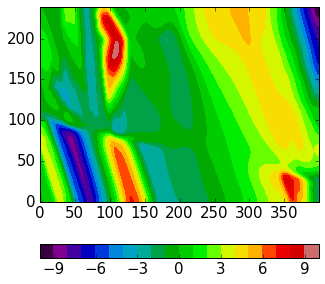
\includegraphics{5-Geophysical-Potential-Fields_31_0.png}
\caption{png}\end{figure}

\begin{Verbatim}[commandchars=\\\{\}]
\PYG{c}{\PYGZsh{} compare sections through model}
\PYG{n}{geo\PYGZus{}changed}\PYG{o}{.}\PYG{n}{plot\PYGZus{}section}\PYG{p}{(}\PYG{l+s}{\PYGZsq{}}\PYG{l+s}{y}\PYG{l+s}{\PYGZsq{}}\PYG{p}{,} \PYG{n}{colorbar} \PYG{o}{=} \PYG{n+nb+bp}{False}\PYG{p}{)}
\PYG{n}{h\PYGZus{}out}\PYG{o}{.}\PYG{n}{plot\PYGZus{}section}\PYG{p}{(}\PYG{l+s}{\PYGZsq{}}\PYG{l+s}{y}\PYG{l+s}{\PYGZsq{}}\PYG{p}{,} \PYG{n}{colorbar} \PYG{o}{=} \PYG{n+nb+bp}{False}\PYG{p}{)}
\end{Verbatim}
\begin{figure}[htbp]
\centering
\capstart

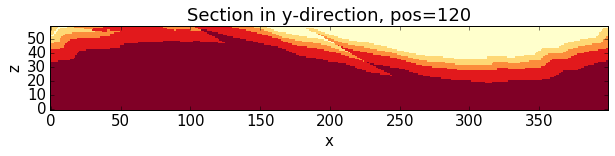
\includegraphics{5-Geophysical-Potential-Fields_32_0.png}
\caption{png}\end{figure}
\begin{figure}[htbp]
\centering
\capstart

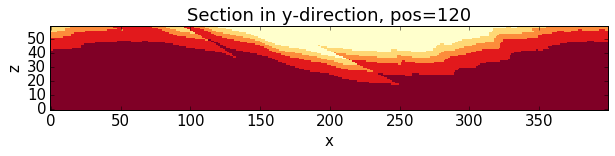
\includegraphics{5-Geophysical-Potential-Fields_32_1.png}
\caption{png}\end{figure}

\begin{Verbatim}[commandchars=\\\{\}]
\PYG{k}{for} \PYG{n}{i} \PYG{o+ow}{in} \PYG{n+nb}{range}\PYG{p}{(}\PYG{l+m+mi}{4}\PYG{p}{)}\PYG{p}{:}
    \PYG{k}{print}\PYG{p}{(}\PYG{l+s}{\PYGZdq{}}\PYG{l+s}{Event }\PYG{l+s+si}{\PYGZpc{}d}\PYG{l+s}{\PYGZdq{}} \PYG{o}{\PYGZpc{}} \PYG{p}{(}\PYG{n}{i}\PYG{o}{+}\PYG{l+m+mi}{2}\PYG{p}{)}\PYG{p}{)}
    \PYG{k}{print} \PYG{n}{his}\PYG{o}{.}\PYG{n}{events}\PYG{p}{[}\PYG{n}{i}\PYG{o}{+}\PYG{l+m+mi}{2}\PYG{p}{]}\PYG{o}{.}\PYG{n}{properties}\PYG{p}{[}\PYG{l+s}{\PYGZsq{}}\PYG{l+s}{Slip}\PYG{l+s}{\PYGZsq{}}\PYG{p}{]}
    \PYG{k}{print} \PYG{n}{his}\PYG{o}{.}\PYG{n}{events}\PYG{p}{[}\PYG{n}{i}\PYG{o}{+}\PYG{l+m+mi}{2}\PYG{p}{]}\PYG{o}{.}\PYG{n}{properties}\PYG{p}{[}\PYG{l+s}{\PYGZsq{}}\PYG{l+s}{Dip}\PYG{l+s}{\PYGZsq{}}\PYG{p}{]}
    \PYG{k}{print} \PYG{n}{his}\PYG{o}{.}\PYG{n}{events}\PYG{p}{[}\PYG{n}{i}\PYG{o}{+}\PYG{l+m+mi}{2}\PYG{p}{]}\PYG{o}{.}\PYG{n}{properties}\PYG{p}{[}\PYG{l+s}{\PYGZsq{}}\PYG{l+s}{Dip Direction}\PYG{l+s}{\PYGZsq{}}\PYG{p}{]}
\end{Verbatim}

\begin{Verbatim}[commandchars=\\\{\}]
Event 2
\PYGZhy{}5000.0
0.0
90.0
Event 3
\PYGZhy{}3000.0
0.0
90.0
Event 4
\PYGZhy{}3000.0
0.0
90.0
Event 5
12000.0
80.0
170.0
\end{Verbatim}

\begin{Verbatim}[commandchars=\\\{\}]
\PYG{c}{\PYGZsh{} recompute the geology blocks for comparison:}
\PYG{n}{pynoddy}\PYG{o}{.}\PYG{n}{compute\PYGZus{}model}\PYG{p}{(}\PYG{l+s}{\PYGZsq{}}\PYG{l+s}{fold\PYGZus{}thrust\PYGZus{}changed.his}\PYG{l+s}{\PYGZsq{}}\PYG{p}{,} \PYG{l+s}{\PYGZsq{}}\PYG{l+s}{fold\PYGZus{}thrust\PYGZus{}changed\PYGZus{}out}\PYG{l+s}{\PYGZsq{}}\PYG{p}{)}
\end{Verbatim}

\begin{Verbatim}[commandchars=\\\{\}]
\PYG{l+s}{\PYGZsq{}}\PYG{l+s}{\PYGZsq{}}
\end{Verbatim}

\begin{Verbatim}[commandchars=\\\{\}]
\PYG{n}{geology\PYGZus{}changed} \PYG{o}{=} \PYG{n}{pynoddy}\PYG{o}{.}\PYG{n}{output}\PYG{o}{.}\PYG{n}{NoddyOutput}\PYG{p}{(}\PYG{l+s}{\PYGZsq{}}\PYG{l+s}{fold\PYGZus{}thrust\PYGZus{}changed\PYGZus{}out}\PYG{l+s}{\PYGZsq{}}\PYG{p}{)}
\end{Verbatim}

\begin{Verbatim}[commandchars=\\\{\}]
\PYG{n}{geology\PYGZus{}changed}\PYG{o}{.}\PYG{n}{plot\PYGZus{}section}\PYG{p}{(}\PYG{l+s}{\PYGZsq{}}\PYG{l+s}{x}\PYG{l+s}{\PYGZsq{}}\PYG{p}{,}
\PYG{c}{\PYGZsh{}                    layer\PYGZus{}labels = his.model\PYGZus{}stratigraphy,}
                   \PYG{n}{colorbar\PYGZus{}orientation} \PYG{o}{=} \PYG{l+s}{\PYGZsq{}}\PYG{l+s}{horizontal}\PYG{l+s}{\PYGZsq{}}\PYG{p}{,}
                   \PYG{n}{colorbar}\PYG{o}{=}\PYG{n+nb+bp}{False}\PYG{p}{,}
                   \PYG{n}{title} \PYG{o}{=} \PYG{l+s}{\PYGZsq{}}\PYG{l+s}{\PYGZsq{}}\PYG{p}{,}
\PYG{c}{\PYGZsh{}                   savefig=True, fig\PYGZus{}filename = \PYGZsq{}fold\PYGZus{}thrust\PYGZus{}NS\PYGZus{}section.eps\PYGZsq{},}
                   \PYG{n}{cmap} \PYG{o}{=} \PYG{l+s}{\PYGZsq{}}\PYG{l+s}{YlOrRd}\PYG{l+s}{\PYGZsq{}}\PYG{p}{)}
\end{Verbatim}
\begin{figure}[htbp]
\centering
\capstart

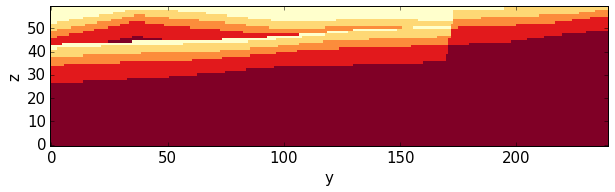
\includegraphics{5-Geophysical-Potential-Fields_36_0.png}
\caption{png}\end{figure}

\begin{Verbatim}[commandchars=\\\{\}]
\PYG{n}{geology\PYGZus{}changed}\PYG{o}{.}\PYG{n}{plot\PYGZus{}section}\PYG{p}{(}\PYG{l+s}{\PYGZsq{}}\PYG{l+s}{y}\PYG{l+s}{\PYGZsq{}}\PYG{p}{,}
                             \PYG{c}{\PYGZsh{} layer\PYGZus{}labels = his.model\PYGZus{}stratigraphy,}
                   \PYG{n}{colorbar\PYGZus{}orientation} \PYG{o}{=} \PYG{l+s}{\PYGZsq{}}\PYG{l+s}{horizontal}\PYG{l+s}{\PYGZsq{}}\PYG{p}{,} \PYG{n}{title} \PYG{o}{=} \PYG{l+s}{\PYGZsq{}}\PYG{l+s}{\PYGZsq{}}\PYG{p}{,} \PYG{n}{cmap} \PYG{o}{=} \PYG{l+s}{\PYGZsq{}}\PYG{l+s}{YlOrRd}\PYG{l+s}{\PYGZsq{}}\PYG{p}{,}
\PYG{c}{\PYGZsh{}                   savefig=True, fig\PYGZus{}filename = \PYGZsq{}fold\PYGZus{}thrust\PYGZus{}EW\PYGZus{}section.eps\PYGZsq{},}
                   \PYG{n}{ve}\PYG{o}{=}\PYG{l+m+mf}{1.5}\PYG{p}{)}
\end{Verbatim}
\begin{figure}[htbp]
\centering
\capstart

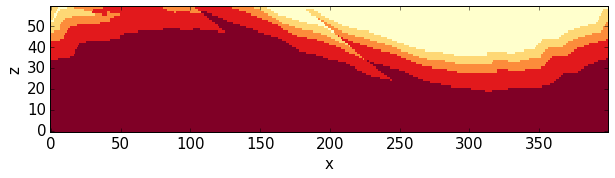
\includegraphics{5-Geophysical-Potential-Fields_37_0.png}
\caption{png}\end{figure}

\begin{Verbatim}[commandchars=\\\{\}]
\PYG{c}{\PYGZsh{} Calculate block difference and export as VTK for 3\PYGZhy{}D visualisation:}
\PYG{k+kn}{import} \PYG{n+nn}{copy}
\PYG{n}{diff\PYGZus{}model} \PYG{o}{=} \PYG{n}{copy}\PYG{o}{.}\PYG{n}{deepcopy}\PYG{p}{(}\PYG{n}{geology\PYGZus{}changed}\PYG{p}{)}
\PYG{n}{diff\PYGZus{}model}\PYG{o}{.}\PYG{n}{block} \PYG{o}{\PYGZhy{}}\PYG{o}{=} \PYG{n}{h\PYGZus{}out}\PYG{o}{.}\PYG{n}{block}
\end{Verbatim}

\begin{Verbatim}[commandchars=\\\{\}]
\PYG{n}{diff\PYGZus{}model}\PYG{o}{.}\PYG{n}{export\PYGZus{}to\PYGZus{}vtk}\PYG{p}{(}\PYG{n}{vtk\PYGZus{}filename} \PYG{o}{=} \PYG{l+s}{\PYGZdq{}}\PYG{l+s}{diff\PYGZus{}model\PYGZus{}fold\PYGZus{}thrust\PYGZus{}belt}\PYG{l+s}{\PYGZdq{}}\PYG{p}{)}
\end{Verbatim}


\section{Figure with all results}
\label{notebooks/5-Geophysical-Potential-Fields:figure-with-all-results}
We now create a figure with the gravity field of the original and the
changed model, as well as a difference plot to highlight areas with
significant changes. This example also shows how additional equations
can easily be combined with pynoddy classes.

\begin{Verbatim}[commandchars=\\\{\}]
\PYG{n}{fig} \PYG{o}{=} \PYG{n}{plt}\PYG{o}{.}\PYG{n}{figure}\PYG{p}{(}\PYG{n}{figsize}\PYG{o}{=}\PYG{p}{(}\PYG{l+m+mi}{20}\PYG{p}{,}\PYG{l+m+mi}{8}\PYG{p}{)}\PYG{p}{)}
\PYG{n}{ax1} \PYG{o}{=} \PYG{n}{fig}\PYG{o}{.}\PYG{n}{add\PYGZus{}subplot}\PYG{p}{(}\PYG{l+m+mi}{131}\PYG{p}{)}
\PYG{c}{\PYGZsh{} original plot}
\PYG{n}{levels} \PYG{o}{=} \PYG{n}{np}\PYG{o}{.}\PYG{n}{arange}\PYG{p}{(}\PYG{l+m+mi}{322}\PYG{p}{,}\PYG{l+m+mi}{344}\PYG{p}{,}\PYG{l+m+mi}{1}\PYG{p}{)}
\PYG{n}{cf1} \PYG{o}{=} \PYG{n}{ax1}\PYG{o}{.}\PYG{n}{contourf}\PYG{p}{(}\PYG{n}{geophys}\PYG{o}{.}\PYG{n}{grv\PYGZus{}data}\PYG{p}{,} \PYG{n}{levels}\PYG{p}{,} \PYG{n}{cmap} \PYG{o}{=} \PYG{l+s}{\PYGZsq{}}\PYG{l+s}{gray}\PYG{l+s}{\PYGZsq{}}\PYG{p}{,} \PYG{n}{vmin} \PYG{o}{=} \PYG{l+m+mi}{324}\PYG{p}{,} \PYG{n}{vmax} \PYG{o}{=} \PYG{l+m+mi}{342}\PYG{p}{)}
\PYG{c}{\PYGZsh{} cbar1 = ax1.colorbar(cf1, orientation = \PYGZsq{}horizontal\PYGZsq{})}
\PYG{n}{fig}\PYG{o}{.}\PYG{n}{colorbar}\PYG{p}{(}\PYG{n}{cf1}\PYG{p}{,} \PYG{n}{orientation}\PYG{o}{=}\PYG{l+s}{\PYGZsq{}}\PYG{l+s}{horizontal}\PYG{l+s}{\PYGZsq{}}\PYG{p}{)}
\PYG{n}{ax1}\PYG{o}{.}\PYG{n}{set\PYGZus{}title}\PYG{p}{(}\PYG{l+s}{\PYGZsq{}}\PYG{l+s}{Gravity of original model}\PYG{l+s}{\PYGZsq{}}\PYG{p}{)}

\PYG{n}{ax2} \PYG{o}{=} \PYG{n}{fig}\PYG{o}{.}\PYG{n}{add\PYGZus{}subplot}\PYG{p}{(}\PYG{l+m+mi}{132}\PYG{p}{)}




\PYG{n}{cf2} \PYG{o}{=} \PYG{n}{ax2}\PYG{o}{.}\PYG{n}{contourf}\PYG{p}{(}\PYG{n}{geophys\PYGZus{}changed}\PYG{o}{.}\PYG{n}{grv\PYGZus{}data}\PYG{p}{,} \PYG{n}{levels}\PYG{p}{,} \PYG{n}{cmap} \PYG{o}{=} \PYG{l+s}{\PYGZsq{}}\PYG{l+s}{gray}\PYG{l+s}{\PYGZsq{}}\PYG{p}{,} \PYG{n}{vmin} \PYG{o}{=} \PYG{l+m+mi}{324}\PYG{p}{,} \PYG{n}{vmax} \PYG{o}{=} \PYG{l+m+mi}{342}\PYG{p}{)}
\PYG{n}{ax2}\PYG{o}{.}\PYG{n}{set\PYGZus{}title}\PYG{p}{(}\PYG{l+s}{\PYGZsq{}}\PYG{l+s}{Gravity of changed model}\PYG{l+s}{\PYGZsq{}}\PYG{p}{)}
\PYG{n}{fig}\PYG{o}{.}\PYG{n}{colorbar}\PYG{p}{(}\PYG{n}{cf2}\PYG{p}{,} \PYG{n}{orientation}\PYG{o}{=}\PYG{l+s}{\PYGZsq{}}\PYG{l+s}{horizontal}\PYG{l+s}{\PYGZsq{}}\PYG{p}{)}

\PYG{n}{ax3} \PYG{o}{=} \PYG{n}{fig}\PYG{o}{.}\PYG{n}{add\PYGZus{}subplot}\PYG{p}{(}\PYG{l+m+mi}{133}\PYG{p}{)}


\PYG{n}{comp\PYGZus{}levels} \PYG{o}{=} \PYG{n}{np}\PYG{o}{.}\PYG{n}{arange}\PYG{p}{(}\PYG{o}{\PYGZhy{}}\PYG{l+m+mf}{10.}\PYG{p}{,}\PYG{l+m+mf}{10.1}\PYG{p}{,}\PYG{l+m+mf}{0.25}\PYG{p}{)}
\PYG{n}{cf3} \PYG{o}{=} \PYG{n}{ax3}\PYG{o}{.}\PYG{n}{contourf}\PYG{p}{(}\PYG{n}{geophys}\PYG{o}{.}\PYG{n}{grv\PYGZus{}data} \PYG{o}{\PYGZhy{}} \PYG{n}{geophys\PYGZus{}changed}\PYG{o}{.}\PYG{n}{grv\PYGZus{}data}\PYG{p}{,} \PYG{n}{comp\PYGZus{}levels}\PYG{p}{,} \PYG{n}{cmap} \PYG{o}{=} \PYG{l+s}{\PYGZsq{}}\PYG{l+s}{RdBu\PYGZus{}r}\PYG{l+s}{\PYGZsq{}}\PYG{p}{)}
\PYG{n}{ax3}\PYG{o}{.}\PYG{n}{set\PYGZus{}title}\PYG{p}{(}\PYG{l+s}{\PYGZsq{}}\PYG{l+s}{Gravity difference}\PYG{l+s}{\PYGZsq{}}\PYG{p}{)}

\PYG{n}{fig}\PYG{o}{.}\PYG{n}{colorbar}\PYG{p}{(}\PYG{n}{cf3}\PYG{p}{,} \PYG{n}{orientation}\PYG{o}{=}\PYG{l+s}{\PYGZsq{}}\PYG{l+s}{horizontal}\PYG{l+s}{\PYGZsq{}}\PYG{p}{)}

\PYG{n}{plt}\PYG{o}{.}\PYG{n}{savefig}\PYG{p}{(}\PYG{l+s}{\PYGZdq{}}\PYG{l+s}{grav\PYGZus{}ori\PYGZus{}changed\PYGZus{}compared.eps}\PYG{l+s}{\PYGZdq{}}\PYG{p}{)}
\end{Verbatim}
\begin{figure}[htbp]
\centering
\capstart

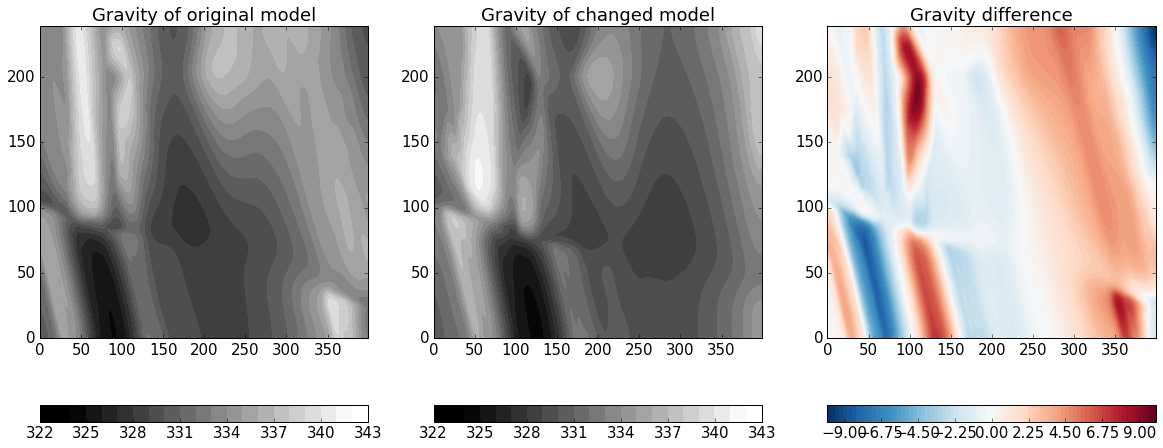
\includegraphics{5-Geophysical-Potential-Fields_41_0.png}
\caption{png}\end{figure}


\chapter{Reproducible Experiments with pynoddy}
\label{notebooks/6-Reproducible-Experiments:reproducible-experiments-with-pynoddy}\label{notebooks/6-Reproducible-Experiments::doc}
All \code{pynoddy} experiments can be defined in a Python script, and if
all settings are appropriate, then this script can be re-run to obtain a
reproduction of the results. However, it is often more convenient to
encapsulate all elements of an experiment within one class. We show here
how this is done in the \code{pynoddy.experiment.Experiment} class and how
this class can be used to define simple reproducible experiments with
kinematic models.

\begin{Verbatim}[commandchars=\\\{\}]
\PYG{k+kn}{from} \PYG{n+nn}{IPython.core.display} \PYG{k+kn}{import} \PYG{n}{HTML}
\PYG{n}{css\PYGZus{}file} \PYG{o}{=} \PYG{l+s}{\PYGZsq{}}\PYG{l+s}{pynoddy.css}\PYG{l+s}{\PYGZsq{}}
\PYG{n}{HTML}\PYG{p}{(}\PYG{n+nb}{open}\PYG{p}{(}\PYG{n}{css\PYGZus{}file}\PYG{p}{,} \PYG{l+s}{\PYGZdq{}}\PYG{l+s}{r}\PYG{l+s}{\PYGZdq{}}\PYG{p}{)}\PYG{o}{.}\PYG{n}{read}\PYG{p}{(}\PYG{p}{)}\PYG{p}{)}
\end{Verbatim}

\begin{Verbatim}[commandchars=\\\{\}]
\PYGZpc{}matplotlib inline
\end{Verbatim}

\begin{Verbatim}[commandchars=\\\{\}]
\PYG{c}{\PYGZsh{} here the usual imports. If any of the imports fails, make sure that pynoddy is installed}
\PYG{c}{\PYGZsh{} properly, ideally with \PYGZsq{}python setup.py develop\PYGZsq{} or \PYGZsq{}python setup.py install\PYGZsq{}}
\PYG{k+kn}{import} \PYG{n+nn}{sys}\PYG{o}{,} \PYG{n+nn}{os}
\PYG{k+kn}{import} \PYG{n+nn}{matplotlib.pyplot} \PYG{k+kn}{as} \PYG{n+nn}{plt}
\PYG{k+kn}{import} \PYG{n+nn}{numpy} \PYG{k+kn}{as} \PYG{n+nn}{np}
\PYG{c}{\PYGZsh{} adjust some settings for matplotlib}
\PYG{k+kn}{from} \PYG{n+nn}{matplotlib} \PYG{k+kn}{import} \PYG{n}{rcParams}
\PYG{c}{\PYGZsh{} print rcParams}
\PYG{n}{rcParams}\PYG{p}{[}\PYG{l+s}{\PYGZsq{}}\PYG{l+s}{font.size}\PYG{l+s}{\PYGZsq{}}\PYG{p}{]} \PYG{o}{=} \PYG{l+m+mi}{15}
\PYG{c}{\PYGZsh{} determine path of repository to set paths corretly below}
\PYG{n}{repo\PYGZus{}path} \PYG{o}{=} \PYG{n}{os}\PYG{o}{.}\PYG{n}{path}\PYG{o}{.}\PYG{n}{realpath}\PYG{p}{(}\PYG{l+s}{\PYGZsq{}}\PYG{l+s}{../..}\PYG{l+s}{\PYGZsq{}}\PYG{p}{)}
\PYG{k+kn}{import} \PYG{n+nn}{pynoddy.history}
\PYG{k+kn}{import} \PYG{n+nn}{pynoddy.experiment}
\PYG{n+nb}{reload}\PYG{p}{(}\PYG{n}{pynoddy}\PYG{o}{.}\PYG{n}{experiment}\PYG{p}{)}
\PYG{n}{rcParams}\PYG{o}{.}\PYG{n}{update}\PYG{p}{(}\PYG{p}{\PYGZob{}}\PYG{l+s}{\PYGZsq{}}\PYG{l+s}{font.size}\PYG{l+s}{\PYGZsq{}}\PYG{p}{:} \PYG{l+m+mi}{15}\PYG{p}{\PYGZcb{}}\PYG{p}{)}
\end{Verbatim}


\section{Defining an experiment}
\label{notebooks/6-Reproducible-Experiments:defining-an-experiment}
We are considering the following scenario: we defined a kinematic model
of a prospective geological unit at depth. As we know that the estimates
of the (kinematic) model parameters contain a high degree of
uncertainty, we would like to represent this uncertainty with the model.

Our approach is here to perform a randomised uncertainty propagation
analysis with a Monte Carlo sampling method. Results should be presented
in several figures (2-D slice plots and a VTK representation in 3-D).

To perform this analysis, we need to perform the following steps (see
main paper for more details):
\begin{enumerate}
\item {} 
Define kinematic model parameters and construct the initial (base)
model;

\item {} 
Assign probability distributions (and possible parameter
correlations) to relevant uncertain input parameters;

\item {} 
Generate a set of n random realisations, repeating the following
steps:
\begin{enumerate}
\item {} 
Draw a randomised input parameter set from the parameter distribu-
tion;

\item {} 
Generate a model with this parameter set;

\item {} 
Analyse the generated model and store results;

\end{enumerate}

\item {} 
Finally: perform postprocessing, generate figures of results

\end{enumerate}

It would be possible to write a Python script to perform all of these
steps in one go. However, we will here take another path and use the
implementation in a Pynoddy Experiment class. Initially, this requires
more work and a careful definition of the experiment - but, finally, it
will enable a higher level of flexibility, extensibility, and
reproducibility.


\section{Setting up the experiment class}
\label{notebooks/6-Reproducible-Experiments:setting-up-the-experiment-class}
We use an experiment class that is pre-defined in the pynoddy.experiment
module and inherits many base functions from the Experiment-class
definition.


\section{Loading an example model from the Virtual Explorer Atlas}
\label{notebooks/6-Reproducible-Experiments:loading-an-example-model-from-the-virtual-explorer-atlas}
As in the last example, we will use a model from the Virtual Explorer
Atlas as an examlpe model for this simulation. We use a model for a fold
interference structure. A discretised 3-D version of this model (from
the Virtual Explorer website) is presented in the figure below. The
model represents a fold interference pattern of ``Type 1'' according to
the definition of Ramsey (1967).
\begin{figure}[htbp]
\centering
\end{figure}

Instead of loading the model into a history object, we are now directly
creating an experiment object for the type of uncertainty analysis:

\begin{Verbatim}[commandchars=\\\{\}]
\PYG{n+nb}{reload}\PYG{p}{(}\PYG{n}{pynoddy}\PYG{o}{.}\PYG{n}{history}\PYG{p}{)}
\PYG{n+nb}{reload}\PYG{p}{(}\PYG{n}{pynoddy}\PYG{o}{.}\PYG{n}{experiment}\PYG{p}{)}

\PYG{k+kn}{from} \PYG{n+nn}{pynoddy.experiment} \PYG{k+kn}{import} \PYG{n}{UncertaintyAnalysis}
\PYG{n+nb}{reload}\PYG{p}{(}\PYG{n}{UncertaintyAnalysis}\PYG{p}{)}
\PYG{c}{\PYGZsh{} model\PYGZus{}url = \PYGZsq{}http://virtualexplorer.com.au/special/noddyatlas/ch3/ch3\PYGZus{}7/his/typeb.his\PYGZsq{}}
\PYG{n}{model\PYGZus{}url} \PYG{o}{=} \PYG{l+s}{\PYGZsq{}}\PYG{l+s}{http://tectonique.net/asg/ch3/ch3\PYGZus{}7/his/typeb.his}\PYG{l+s}{\PYGZsq{}}
\PYG{n}{ue} \PYG{o}{=} \PYG{n}{UncertaintyAnalysis}\PYG{o}{.}\PYG{n}{UncertaintyAnalysis}\PYG{p}{(}\PYG{n}{url} \PYG{o}{=} \PYG{n}{model\PYGZus{}url}\PYG{p}{)}
\PYG{c}{\PYGZsh{} ue = pynoddy.experiment.UncertaintyAnalysis(history = \PYGZdq{}typeb\PYGZus{}tmp.his\PYGZdq{})}
\end{Verbatim}

\begin{Verbatim}[commandchars=\\\{\}]
\PYGZhy{}\PYGZhy{}\PYGZhy{}\PYGZhy{}\PYGZhy{}\PYGZhy{}\PYGZhy{}\PYGZhy{}\PYGZhy{}\PYGZhy{}\PYGZhy{}\PYGZhy{}\PYGZhy{}\PYGZhy{}\PYGZhy{}\PYGZhy{}\PYGZhy{}\PYGZhy{}\PYGZhy{}\PYGZhy{}\PYGZhy{}\PYGZhy{}\PYGZhy{}\PYGZhy{}\PYGZhy{}\PYGZhy{}\PYGZhy{}\PYGZhy{}\PYGZhy{}\PYGZhy{}\PYGZhy{}\PYGZhy{}\PYGZhy{}\PYGZhy{}\PYGZhy{}\PYGZhy{}\PYGZhy{}\PYGZhy{}\PYGZhy{}\PYGZhy{}\PYGZhy{}\PYGZhy{}\PYGZhy{}\PYGZhy{}\PYGZhy{}\PYGZhy{}\PYGZhy{}\PYGZhy{}\PYGZhy{}\PYGZhy{}\PYGZhy{}\PYGZhy{}\PYGZhy{}\PYGZhy{}\PYGZhy{}\PYGZhy{}\PYGZhy{}\PYGZhy{}\PYGZhy{}\PYGZhy{}\PYGZhy{}\PYGZhy{}\PYGZhy{}\PYGZhy{}\PYGZhy{}\PYGZhy{}\PYGZhy{}\PYGZhy{}\PYGZhy{}\PYGZhy{}\PYGZhy{}\PYGZhy{}\PYGZhy{}\PYGZhy{}\PYGZhy{}

TypeError                                 Traceback (most recent call last)

\PYGZlt{}ipython\PYGZhy{}input\PYGZhy{}4\PYGZhy{}0906eece45d0\PYGZgt{} in \PYGZlt{}module\PYGZgt{}()
      6 \PYGZsh{} model\PYGZus{}url = \PYGZsq{}http://virtualexplorer.com.au/special/noddyatlas/ch3/ch3\PYGZus{}7/his/typeb.his\PYGZsq{}
      7 model\PYGZus{}url = \PYGZsq{}http://tectonique.net/asg/ch3/ch3\PYGZus{}7/his/typeb.his\PYGZsq{}
\PYGZhy{}\PYGZhy{}\PYGZhy{}\PYGZhy{}\PYGZgt{} 8 ue = UncertaintyAnalysis.UncertaintyAnalysis(url = model\PYGZus{}url)
      9 \PYGZsh{} ue = pynoddy.experiment.UncertaintyAnalysis(history = \PYGZdq{}typeb\PYGZus{}tmp.his\PYGZdq{})


TypeError: \PYGZus{}\PYGZus{}init\PYGZus{}\PYGZus{}() got an unexpected keyword argument \PYGZsq{}url\PYGZsq{}
\end{Verbatim}

For simpler visualisation in this notebook, we will analyse the
following steps in a section view of the model.

We consider a section in y-direction through the model:

\begin{Verbatim}[commandchars=\\\{\}]
\PYG{n}{ue}\PYG{o}{.}\PYG{n}{write\PYGZus{}history}\PYG{p}{(}\PYG{l+s}{\PYGZdq{}}\PYG{l+s}{typeb\PYGZus{}tmp3.his}\PYG{l+s}{\PYGZdq{}}\PYG{p}{)}
\end{Verbatim}

\begin{Verbatim}[commandchars=\\\{\}]
\PYG{n}{ue}\PYG{o}{.}\PYG{n}{write\PYGZus{}history}\PYG{p}{(}\PYG{l+s}{\PYGZdq{}}\PYG{l+s}{typeb\PYGZus{}tmp2.his}\PYG{l+s}{\PYGZdq{}}\PYG{p}{)}
\end{Verbatim}

\begin{Verbatim}[commandchars=\\\{\}]
\PYG{n}{ue}\PYG{o}{.}\PYG{n}{change\PYGZus{}cube\PYGZus{}size}\PYG{p}{(}\PYG{l+m+mi}{100}\PYG{p}{)}
\PYG{n}{ue}\PYG{o}{.}\PYG{n}{plot\PYGZus{}section}\PYG{p}{(}\PYG{l+s}{\PYGZsq{}}\PYG{l+s}{y}\PYG{l+s}{\PYGZsq{}}\PYG{p}{)}
\end{Verbatim}
\begin{figure}[htbp]
\centering
\capstart

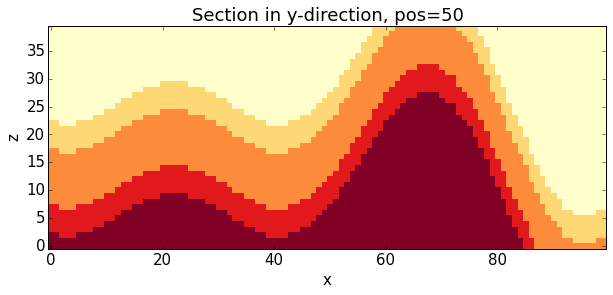
\includegraphics{6-Reproducible-Experiments_11_0.png}
\caption{png}\end{figure}

Before we start to draw random realisations of the model, we should
first store the base state of the model for later reference. This is
simply possibel with the freeze() method which stores the current state
of the model as the ``base-state'':

\begin{Verbatim}[commandchars=\\\{\}]
\PYG{n}{ue}\PYG{o}{.}\PYG{n}{freeze}\PYG{p}{(}\PYG{p}{)}
\end{Verbatim}

We now intialise the random generator. We can directly assign a random
seed to simplify reproducibility (note that this is not \emph{essential}, as
it would be for the definition in a script function: the random state is
preserved within the model and could be retrieved at a later stage, as
well!):

\begin{Verbatim}[commandchars=\\\{\}]
\PYG{n}{ue}\PYG{o}{.}\PYG{n}{set\PYGZus{}random\PYGZus{}seed}\PYG{p}{(}\PYG{l+m+mi}{12345}\PYG{p}{)}
\end{Verbatim}

The next step is to define probability distributions to the relevant
event parameters. Let's first look at the different events:

\begin{Verbatim}[commandchars=\\\{\}]
\PYG{n}{ue}\PYG{o}{.}\PYG{n}{info}\PYG{p}{(}\PYG{n}{events\PYGZus{}only} \PYG{o}{=} \PYG{n+nb+bp}{True}\PYG{p}{)}
\end{Verbatim}

\begin{Verbatim}[commandchars=\\\{\}]
This model consists of 3 events:
    (1) \PYGZhy{} STRATIGRAPHY
    (2) \PYGZhy{} FOLD
    (3) \PYGZhy{} FOLD
\end{Verbatim}

\begin{Verbatim}[commandchars=\\\{\}]
\PYG{n}{ev2} \PYG{o}{=} \PYG{n}{ue}\PYG{o}{.}\PYG{n}{events}\PYG{p}{[}\PYG{l+m+mi}{2}\PYG{p}{]}
\end{Verbatim}

\begin{Verbatim}[commandchars=\\\{\}]
\PYG{n}{ev2}\PYG{o}{.}\PYG{n}{properties}
\end{Verbatim}

\begin{Verbatim}[commandchars=\\\{\}]
\PYG{p}{\PYGZob{}}\PYG{l+s}{\PYGZsq{}}\PYG{l+s}{Amplitude}\PYG{l+s}{\PYGZsq{}}\PYG{p}{:} \PYG{l+m+mf}{1250.0}\PYG{p}{,}
 \PYG{l+s}{\PYGZsq{}}\PYG{l+s}{Cylindricity}\PYG{l+s}{\PYGZsq{}}\PYG{p}{:} \PYG{l+m+mf}{0.0}\PYG{p}{,}
 \PYG{l+s}{\PYGZsq{}}\PYG{l+s}{Dip}\PYG{l+s}{\PYGZsq{}}\PYG{p}{:} \PYG{l+m+mf}{90.0}\PYG{p}{,}
 \PYG{l+s}{\PYGZsq{}}\PYG{l+s}{Dip Direction}\PYG{l+s}{\PYGZsq{}}\PYG{p}{:} \PYG{l+m+mf}{90.0}\PYG{p}{,}
 \PYG{l+s}{\PYGZsq{}}\PYG{l+s}{Pitch}\PYG{l+s}{\PYGZsq{}}\PYG{p}{:} \PYG{l+m+mf}{0.0}\PYG{p}{,}
 \PYG{l+s}{\PYGZsq{}}\PYG{l+s}{Single Fold}\PYG{l+s}{\PYGZsq{}}\PYG{p}{:} \PYG{l+s}{\PYGZsq{}}\PYG{l+s}{FALSE}\PYG{l+s}{\PYGZsq{}}\PYG{p}{,}
 \PYG{l+s}{\PYGZsq{}}\PYG{l+s}{Type}\PYG{l+s}{\PYGZsq{}}\PYG{p}{:} \PYG{l+s}{\PYGZsq{}}\PYG{l+s}{Sine}\PYG{l+s}{\PYGZsq{}}\PYG{p}{,}
 \PYG{l+s}{\PYGZsq{}}\PYG{l+s}{Wavelength}\PYG{l+s}{\PYGZsq{}}\PYG{p}{:} \PYG{l+m+mf}{5000.0}\PYG{p}{,}
 \PYG{l+s}{\PYGZsq{}}\PYG{l+s}{X}\PYG{l+s}{\PYGZsq{}}\PYG{p}{:} \PYG{l+m+mf}{1000.0}\PYG{p}{,}
 \PYG{l+s}{\PYGZsq{}}\PYG{l+s}{Y}\PYG{l+s}{\PYGZsq{}}\PYG{p}{:} \PYG{l+m+mf}{0.0}\PYG{p}{,}
 \PYG{l+s}{\PYGZsq{}}\PYG{l+s}{Z}\PYG{l+s}{\PYGZsq{}}\PYG{p}{:} \PYG{l+m+mf}{0.0}\PYG{p}{\PYGZcb{}}
\end{Verbatim}

Next, we define the probability distributions for the uncertain input
parameters:

\begin{Verbatim}[commandchars=\\\{\}]
\PYG{n}{param\PYGZus{}stats} \PYG{o}{=} \PYG{p}{[}\PYG{p}{\PYGZob{}}\PYG{l+s}{\PYGZsq{}}\PYG{l+s}{event}\PYG{l+s}{\PYGZsq{}} \PYG{p}{:} \PYG{l+m+mi}{2}\PYG{p}{,}
              \PYG{l+s}{\PYGZsq{}}\PYG{l+s}{parameter}\PYG{l+s}{\PYGZsq{}}\PYG{p}{:} \PYG{l+s}{\PYGZsq{}}\PYG{l+s}{Amplitude}\PYG{l+s}{\PYGZsq{}}\PYG{p}{,}
              \PYG{l+s}{\PYGZsq{}}\PYG{l+s}{stdev}\PYG{l+s}{\PYGZsq{}}\PYG{p}{:} \PYG{l+m+mf}{100.0}\PYG{p}{,}
              \PYG{l+s}{\PYGZsq{}}\PYG{l+s}{type}\PYG{l+s}{\PYGZsq{}}\PYG{p}{:} \PYG{l+s}{\PYGZsq{}}\PYG{l+s}{normal}\PYG{l+s}{\PYGZsq{}}\PYG{p}{\PYGZcb{}}\PYG{p}{,}
              \PYG{p}{\PYGZob{}}\PYG{l+s}{\PYGZsq{}}\PYG{l+s}{event}\PYG{l+s}{\PYGZsq{}} \PYG{p}{:} \PYG{l+m+mi}{2}\PYG{p}{,}
              \PYG{l+s}{\PYGZsq{}}\PYG{l+s}{parameter}\PYG{l+s}{\PYGZsq{}}\PYG{p}{:} \PYG{l+s}{\PYGZsq{}}\PYG{l+s}{Wavelength}\PYG{l+s}{\PYGZsq{}}\PYG{p}{,}
              \PYG{l+s}{\PYGZsq{}}\PYG{l+s}{stdev}\PYG{l+s}{\PYGZsq{}}\PYG{p}{:} \PYG{l+m+mf}{500.0}\PYG{p}{,}
              \PYG{l+s}{\PYGZsq{}}\PYG{l+s}{type}\PYG{l+s}{\PYGZsq{}}\PYG{p}{:} \PYG{l+s}{\PYGZsq{}}\PYG{l+s}{normal}\PYG{l+s}{\PYGZsq{}}\PYG{p}{\PYGZcb{}}\PYG{p}{,}
              \PYG{p}{\PYGZob{}}\PYG{l+s}{\PYGZsq{}}\PYG{l+s}{event}\PYG{l+s}{\PYGZsq{}} \PYG{p}{:} \PYG{l+m+mi}{2}\PYG{p}{,}
              \PYG{l+s}{\PYGZsq{}}\PYG{l+s}{parameter}\PYG{l+s}{\PYGZsq{}}\PYG{p}{:} \PYG{l+s}{\PYGZsq{}}\PYG{l+s}{X}\PYG{l+s}{\PYGZsq{}}\PYG{p}{,}
              \PYG{l+s}{\PYGZsq{}}\PYG{l+s}{stdev}\PYG{l+s}{\PYGZsq{}}\PYG{p}{:} \PYG{l+m+mf}{500.0}\PYG{p}{,}
              \PYG{l+s}{\PYGZsq{}}\PYG{l+s}{type}\PYG{l+s}{\PYGZsq{}}\PYG{p}{:} \PYG{l+s}{\PYGZsq{}}\PYG{l+s}{normal}\PYG{l+s}{\PYGZsq{}}\PYG{p}{\PYGZcb{}}\PYG{p}{]}

\PYG{n}{ue}\PYG{o}{.}\PYG{n}{set\PYGZus{}parameter\PYGZus{}statistics}\PYG{p}{(}\PYG{n}{param\PYGZus{}stats}\PYG{p}{)}
\end{Verbatim}

\begin{Verbatim}[commandchars=\\\{\}]
\PYG{n}{resolution} \PYG{o}{=} \PYG{l+m+mi}{100}
\PYG{n}{ue}\PYG{o}{.}\PYG{n}{change\PYGZus{}cube\PYGZus{}size}\PYG{p}{(}\PYG{n}{resolution}\PYG{p}{)}
\PYG{n}{tmp} \PYG{o}{=} \PYG{n}{ue}\PYG{o}{.}\PYG{n}{get\PYGZus{}section}\PYG{p}{(}\PYG{l+s}{\PYGZsq{}}\PYG{l+s}{y}\PYG{l+s}{\PYGZsq{}}\PYG{p}{)}
\PYG{n}{prob\PYGZus{}4} \PYG{o}{=} \PYG{n}{np}\PYG{o}{.}\PYG{n}{zeros\PYGZus{}like}\PYG{p}{(}\PYG{n}{tmp}\PYG{o}{.}\PYG{n}{block}\PYG{p}{[}\PYG{p}{:}\PYG{p}{,}\PYG{p}{:}\PYG{p}{,}\PYG{p}{:}\PYG{p}{]}\PYG{p}{)}
\PYG{n}{n\PYGZus{}draws} \PYG{o}{=} \PYG{l+m+mi}{10}


\PYG{k}{for} \PYG{n}{i} \PYG{o+ow}{in} \PYG{n+nb}{range}\PYG{p}{(}\PYG{n}{n\PYGZus{}draws}\PYG{p}{)}\PYG{p}{:}
    \PYG{n}{ue}\PYG{o}{.}\PYG{n}{random\PYGZus{}draw}\PYG{p}{(}\PYG{p}{)}
    \PYG{n}{tmp} \PYG{o}{=} \PYG{n}{ue}\PYG{o}{.}\PYG{n}{get\PYGZus{}section}\PYG{p}{(}\PYG{l+s}{\PYGZsq{}}\PYG{l+s}{y}\PYG{l+s}{\PYGZsq{}}\PYG{p}{,} \PYG{n}{resolution} \PYG{o}{=} \PYG{n}{resolution}\PYG{p}{)}
    \PYG{n}{prob\PYGZus{}4} \PYG{o}{+}\PYG{o}{=} \PYG{p}{(}\PYG{n}{tmp}\PYG{o}{.}\PYG{n}{block}\PYG{p}{[}\PYG{p}{:}\PYG{p}{,}\PYG{p}{:}\PYG{p}{,}\PYG{p}{:}\PYG{p}{]} \PYG{o}{==} \PYG{l+m+mi}{4}\PYG{p}{)}

\PYG{c}{\PYGZsh{} Normalise}
\PYG{n}{prob\PYGZus{}4} \PYG{o}{=} \PYG{n}{prob\PYGZus{}4} \PYG{o}{/} \PYG{n+nb}{float}\PYG{p}{(}\PYG{n}{n\PYGZus{}draws}\PYG{p}{)}
\end{Verbatim}

\begin{Verbatim}[commandchars=\\\{\}]
\PYG{n}{fig} \PYG{o}{=} \PYG{n}{plt}\PYG{o}{.}\PYG{n}{figure}\PYG{p}{(}\PYG{n}{figsize} \PYG{o}{=} \PYG{p}{(}\PYG{l+m+mi}{12}\PYG{p}{,}\PYG{l+m+mi}{8}\PYG{p}{)}\PYG{p}{)}
\PYG{n}{ax} \PYG{o}{=} \PYG{n}{fig}\PYG{o}{.}\PYG{n}{add\PYGZus{}subplot}\PYG{p}{(}\PYG{l+m+mi}{111}\PYG{p}{)}
\PYG{n}{ax}\PYG{o}{.}\PYG{n}{imshow}\PYG{p}{(}\PYG{n}{prob\PYGZus{}4}\PYG{o}{.}\PYG{n}{transpose}\PYG{p}{(}\PYG{p}{)}\PYG{p}{[}\PYG{p}{:}\PYG{p}{,}\PYG{l+m+mi}{0}\PYG{p}{,}\PYG{p}{:}\PYG{p}{]}\PYG{p}{,}
           \PYG{n}{origin} \PYG{o}{=} \PYG{l+s}{\PYGZsq{}}\PYG{l+s}{lower left}\PYG{l+s}{\PYGZsq{}}\PYG{p}{,}
           \PYG{n}{interpolation} \PYG{o}{=} \PYG{l+s}{\PYGZsq{}}\PYG{l+s}{none}\PYG{l+s}{\PYGZsq{}}\PYG{p}{)}
\PYG{n}{plt}\PYG{o}{.}\PYG{n}{title}\PYG{p}{(}\PYG{l+s}{\PYGZdq{}}\PYG{l+s}{Estimated probability of unit 4}\PYG{l+s}{\PYGZdq{}}\PYG{p}{)}
\PYG{n}{plt}\PYG{o}{.}\PYG{n}{xlabel}\PYG{p}{(}\PYG{l+s}{\PYGZdq{}}\PYG{l+s}{x (E\PYGZhy{}W)}\PYG{l+s}{\PYGZdq{}}\PYG{p}{)}
\PYG{n}{plt}\PYG{o}{.}\PYG{n}{ylabel}\PYG{p}{(}\PYG{l+s}{\PYGZdq{}}\PYG{l+s}{z}\PYG{l+s}{\PYGZdq{}}\PYG{p}{)}
\end{Verbatim}

\begin{Verbatim}[commandchars=\\\{\}]
\PYGZlt{}matplotlib.text.Text at 0x10c0b6a50\PYGZgt{}
\end{Verbatim}
\begin{figure}[htbp]
\centering
\capstart

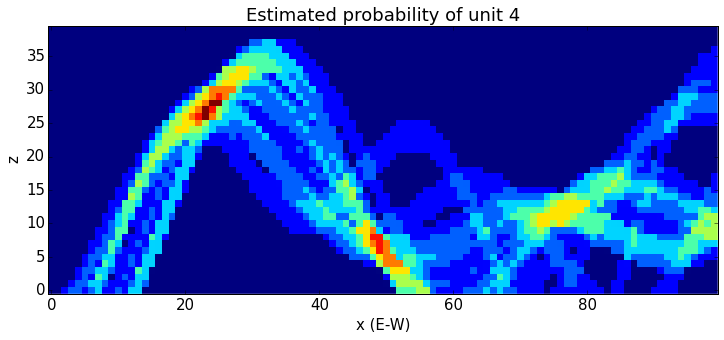
\includegraphics{6-Reproducible-Experiments_23_1.png}
\caption{png}\end{figure}

\begin{Verbatim}[commandchars=\\\{\}]
\PYG{n+nb}{reload}\PYG{p}{(}\PYG{n}{pynoddy}\PYG{o}{.}\PYG{n}{history}\PYG{p}{)}
\PYG{n+nb}{reload}\PYG{p}{(}\PYG{n}{pynoddy}\PYG{o}{.}\PYG{n}{output}\PYG{p}{)}
\PYG{n+nb}{reload}\PYG{p}{(}\PYG{n}{pynoddy}\PYG{o}{.}\PYG{n}{experiment}\PYG{p}{)}
\PYG{n}{model\PYGZus{}url} \PYG{o}{=} \PYG{l+s}{\PYGZsq{}}\PYG{l+s}{http://virtualexplorer.com.au/special/noddyatlas/ch3/ch3\PYGZus{}7/his/typeb.his}\PYG{l+s}{\PYGZsq{}}
\PYG{c}{\PYGZsh{} ue = pynoddy.experiment.UncertaintyAnalysis(url = model\PYGZus{}url)}
\PYG{n}{ue} \PYG{o}{=} \PYG{n}{pynoddy}\PYG{o}{.}\PYG{n}{experiment}\PYG{o}{.}\PYG{n}{UncertaintyAnalysis}\PYG{p}{(}\PYG{n}{history} \PYG{o}{=} \PYG{l+s}{\PYGZdq{}}\PYG{l+s}{typeb\PYGZus{}tmp.his}\PYG{l+s}{\PYGZdq{}}\PYG{p}{)}
\PYG{n}{ue}\PYG{o}{.}\PYG{n}{change\PYGZus{}cube\PYGZus{}size}\PYG{p}{(}\PYG{l+m+mi}{100}\PYG{p}{)}
\PYG{c}{\PYGZsh{} tmp = ue.get\PYGZus{}section(\PYGZsq{}y\PYGZsq{})}
\PYG{c}{\PYGZsh{} tmp.plot\PYGZus{}section(\PYGZsq{}y\PYGZsq{}, position = 0, data = prob\PYGZus{}4, cmap = \PYGZsq{}jet\PYGZsq{})}
\end{Verbatim}

\begin{Verbatim}[commandchars=\\\{\}]
\PYG{n}{STRATIGRAPHY}
\PYG{n}{FOLD}
\PYG{n}{FOLD}
\end{Verbatim}

\begin{Verbatim}[commandchars=\\\{\}]
\PYG{n}{ue}\PYG{o}{.}\PYG{n}{plot\PYGZus{}section}\PYG{p}{(}\PYG{l+s}{\PYGZsq{}}\PYG{l+s}{y}\PYG{l+s}{\PYGZsq{}}\PYG{p}{)}
\end{Verbatim}
\begin{figure}[htbp]
\centering
\capstart

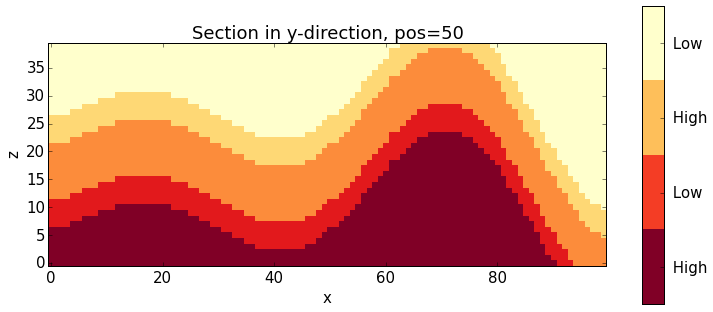
\includegraphics{6-Reproducible-Experiments_25_0.png}
\caption{png}\end{figure}

\begin{Verbatim}[commandchars=\\\{\}]
\PYG{n}{ue}\PYG{o}{.}\PYG{n}{export\PYGZus{}to\PYGZus{}vtk}\PYG{p}{(}\PYG{n}{vtk\PYGZus{}filename} \PYG{o}{=} \PYG{l+s}{\PYGZdq{}}\PYG{l+s}{typeb}\PYG{l+s}{\PYGZdq{}}\PYG{p}{)}
\end{Verbatim}

\begin{Verbatim}[commandchars=\\\{\}]
\PYG{n}{ue}\PYG{o}{.}\PYG{n}{export\PYGZus{}to\PYGZus{}vtk}\PYG{p}{(}\PYG{n}{vtk\PYGZus{}filename} \PYG{o}{=} \PYG{l+s}{\PYGZdq{}}\PYG{l+s}{prob4}\PYG{l+s}{\PYGZdq{}}\PYG{p}{,} \PYG{n}{data} \PYG{o}{=} \PYG{n}{prob\PYGZus{}4}\PYG{p}{)}
\end{Verbatim}

\begin{Verbatim}[commandchars=\\\{\}]
\PYG{n}{pwd}
\end{Verbatim}

\begin{Verbatim}[commandchars=\\\{\}]
\PYG{l+s}{u\PYGZsq{}}\PYG{l+s}{/Users/flow/git/pynoddy/docs/notebooks}\PYG{l+s}{\PYGZsq{}}
\end{Verbatim}

\begin{Verbatim}[commandchars=\\\{\}]
\PYG{n}{block} \PYG{o}{=} \PYG{n}{ue}\PYG{o}{.}\PYG{n}{get\PYGZus{}section}\PYG{p}{(}\PYG{l+s}{\PYGZsq{}}\PYG{l+s}{y}\PYG{l+s}{\PYGZsq{}}\PYG{p}{)}
\end{Verbatim}

\begin{Verbatim}[commandchars=\\\{\}]
\PYG{n}{tmp} \PYG{o}{=} \PYG{n}{np}\PYG{o}{.}\PYG{n}{zeros\PYGZus{}like}\PYG{p}{(}\PYG{n}{block}\PYG{o}{.}\PYG{n}{block}\PYG{p}{)}
\PYG{n}{tmp} \PYG{o}{+}\PYG{o}{=} \PYG{p}{(}\PYG{n}{block}\PYG{o}{.}\PYG{n}{block}\PYG{p}{[}\PYG{p}{:}\PYG{p}{,}\PYG{l+m+mi}{0}\PYG{p}{,}\PYG{p}{:}\PYG{p}{]} \PYG{o}{==} \PYG{l+m+mi}{2}\PYG{p}{)}
\end{Verbatim}

\begin{Verbatim}[commandchars=\\\{\}]
\PYG{n}{plt}\PYG{o}{.}\PYG{n}{imshow}\PYG{p}{(}\PYG{n}{tmp}\PYG{p}{[}\PYG{p}{:}\PYG{p}{,}\PYG{l+m+mi}{0}\PYG{p}{,}\PYG{p}{:}\PYG{p}{]}\PYG{o}{.}\PYG{n}{transpose}\PYG{p}{(}\PYG{p}{)}\PYG{p}{)}
\end{Verbatim}

\begin{Verbatim}[commandchars=\\\{\}]
\PYGZlt{}matplotlib.image.AxesImage at 0x10e9e5750\PYGZgt{}
\end{Verbatim}
\begin{figure}[htbp]
\centering
\capstart

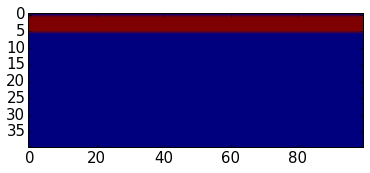
\includegraphics{6-Reproducible-Experiments_31_1.png}
\caption{png}\end{figure}

\begin{Verbatim}[commandchars=\\\{\}]
\PYG{n}{block}\PYG{o}{.}\PYG{n}{plot\PYGZus{}section}\PYG{p}{(}\PYG{l+s}{\PYGZsq{}}\PYG{l+s}{y}\PYG{l+s}{\PYGZsq{}}\PYG{p}{)}
\end{Verbatim}
\begin{figure}[htbp]
\centering
\capstart

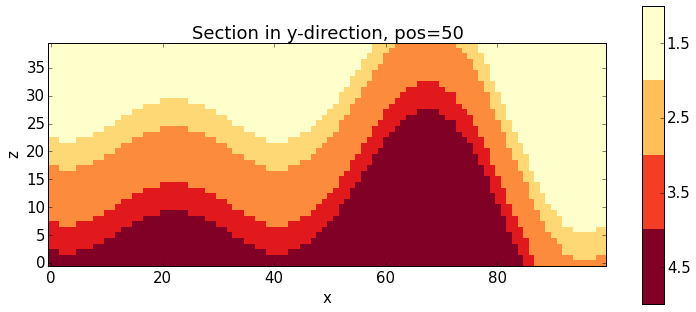
\includegraphics{6-Reproducible-Experiments_32_0.png}
\caption{png}\end{figure}

\begin{Verbatim}[commandchars=\\\{\}]
\PYG{n}{plt}\PYG{o}{.}\PYG{n}{imshow}\PYG{p}{(}\PYG{n}{block}\PYG{o}{.}\PYG{n}{block}\PYG{p}{[}\PYG{p}{:}\PYG{p}{,}\PYG{l+m+mi}{0}\PYG{p}{,}\PYG{p}{:}\PYG{p}{]}\PYG{o}{.}\PYG{n}{transpose}\PYG{p}{(}\PYG{p}{)}\PYG{p}{,} \PYG{n}{origin} \PYG{o}{=} \PYG{l+s}{\PYGZsq{}}\PYG{l+s}{lower left}\PYG{l+s}{\PYGZsq{}}\PYG{p}{,} \PYG{n}{interpolation} \PYG{o}{=} \PYG{l+s}{\PYGZsq{}}\PYG{l+s}{none}\PYG{l+s}{\PYGZsq{}}\PYG{p}{)}
\PYG{n}{plt}\PYG{o}{.}\PYG{n}{colorbar}\PYG{p}{(}\PYG{n}{orientation} \PYG{o}{=} \PYG{l+s}{\PYGZdq{}}\PYG{l+s}{horizontal}\PYG{l+s}{\PYGZdq{}}\PYG{p}{)}
\end{Verbatim}

\begin{Verbatim}[commandchars=\\\{\}]
\PYGZlt{}matplotlib.colorbar.Colorbar instance at 0x10eb97b48\PYGZgt{}
\end{Verbatim}
\begin{figure}[htbp]
\centering
\capstart

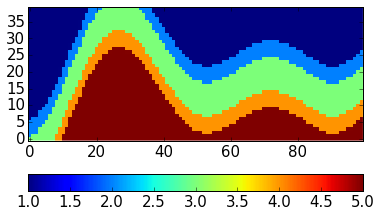
\includegraphics{6-Reproducible-Experiments_33_1.png}
\caption{png}\end{figure}

\begin{Verbatim}[commandchars=\\\{\}]
\PYG{c}{\PYGZsh{} filter out unit 4:}
\PYG{n}{test} \PYG{o}{=} \PYG{n}{np}\PYG{o}{.}\PYG{n}{zeros\PYGZus{}like}\PYG{p}{(}\PYG{n}{block}\PYG{o}{.}\PYG{n}{block}\PYG{p}{[}\PYG{p}{:}\PYG{p}{,}\PYG{l+m+mi}{0}\PYG{p}{,}\PYG{p}{:}\PYG{p}{]}\PYG{p}{)}
\PYG{n}{test} \PYG{o}{+}\PYG{o}{=} \PYG{p}{(}\PYG{n}{block}\PYG{o}{.}\PYG{n}{block}\PYG{p}{[}\PYG{p}{:}\PYG{p}{,}\PYG{l+m+mi}{0}\PYG{p}{,}\PYG{p}{:}\PYG{p}{]} \PYG{o}{==} \PYG{l+m+mi}{4}\PYG{p}{)}
\PYG{n}{plt}\PYG{o}{.}\PYG{n}{imshow}\PYG{p}{(}\PYG{n}{test}\PYG{o}{.}\PYG{n}{transpose}\PYG{p}{(}\PYG{p}{)}\PYG{p}{,} \PYG{n}{origin} \PYG{o}{=} \PYG{l+s}{\PYGZsq{}}\PYG{l+s}{lower left}\PYG{l+s}{\PYGZsq{}}\PYG{p}{,} \PYG{n}{interpolation} \PYG{o}{=} \PYG{l+s}{\PYGZsq{}}\PYG{l+s}{none}\PYG{l+s}{\PYGZsq{}}\PYG{p}{)}
\end{Verbatim}

\begin{Verbatim}[commandchars=\\\{\}]
\PYGZlt{}matplotlib.image.AxesImage at 0x10ed5cc90\PYGZgt{}
\end{Verbatim}
\begin{figure}[htbp]
\centering
\capstart

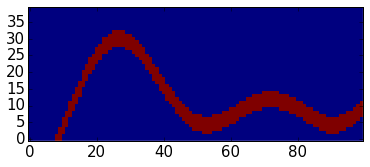
\includegraphics{6-Reproducible-Experiments_34_1.png}
\caption{png}\end{figure}

\begin{Verbatim}[commandchars=\\\{\}]
\PYG{n}{ue}\PYG{o}{.}\PYG{n}{write\PYGZus{}history}\PYG{p}{(}\PYG{l+s}{\PYGZdq{}}\PYG{l+s}{typeb\PYGZus{}tmp.his}\PYG{l+s}{\PYGZdq{}}\PYG{p}{)}
\end{Verbatim}

\begin{Verbatim}[commandchars=\\\{\}]
\PYG{n}{ue}\PYG{o}{.}\PYG{n}{events}\PYG{p}{[}\PYG{l+m+mi}{2}\PYG{p}{]}\PYG{o}{.}\PYG{n}{event\PYGZus{}lines}\PYG{p}{[}\PYG{o}{\PYGZhy{}}\PYG{l+m+mi}{1}\PYG{p}{]}
\end{Verbatim}

\begin{Verbatim}[commandchars=\\\{\}]
\PYG{l+s}{\PYGZsq{}}\PYG{l+s+se}{\PYGZbs{}t}\PYG{l+s}{Name}\PYG{l+s+se}{\PYGZbs{}t}\PYG{l+s}{= Fold}\PYG{l+s+se}{\PYGZbs{}n}\PYG{l+s}{\PYGZsq{}}
\end{Verbatim}

\begin{Verbatim}[commandchars=\\\{\}]
\PYG{k}{for} \PYG{n}{i}\PYG{p}{,}\PYG{n}{line} \PYG{o+ow}{in} \PYG{n+nb}{enumerate}\PYG{p}{(}\PYG{n}{ue}\PYG{o}{.}\PYG{n}{history\PYGZus{}lines}\PYG{p}{)}\PYG{p}{:}
    \PYG{k}{if} \PYG{l+s}{\PYGZsq{}}\PYG{l+s}{BlockOptions}\PYG{l+s}{\PYGZsq{}} \PYG{o+ow}{in} \PYG{n}{line}\PYG{p}{:}
        \PYG{k}{print} \PYG{n}{ue}\PYG{o}{.}\PYG{n}{history\PYGZus{}lines}\PYG{p}{[}\PYG{n}{i}\PYG{o}{\PYGZhy{}}\PYG{l+m+mi}{1}\PYG{p}{]} \PYG{o}{==} \PYG{l+s}{\PYGZsq{}}\PYG{l+s+se}{\PYGZbs{}n}\PYG{l+s}{\PYGZsq{}}
\end{Verbatim}

\begin{Verbatim}[commandchars=\\\{\}]
\PYG{n+nb+bp}{True}
\end{Verbatim}

\begin{Verbatim}[commandchars=\\\{\}]
list.insert??
\end{Verbatim}

\begin{Verbatim}[commandchars=\\\{\}]
\PYG{n}{a} \PYG{o}{=} \PYG{p}{[}\PYG{l+s}{\PYGZsq{}}\PYG{l+s}{a}\PYG{l+s}{\PYGZsq{}}\PYG{p}{,} \PYG{l+s}{\PYGZsq{}}\PYG{l+s}{b}\PYG{l+s}{\PYGZsq{}}\PYG{p}{,} \PYG{l+s}{\PYGZsq{}}\PYG{l+s}{c}\PYG{l+s}{\PYGZsq{}}\PYG{p}{]}
\end{Verbatim}

\begin{Verbatim}[commandchars=\\\{\}]
\PYG{k}{print} \PYG{n}{a}\PYG{p}{[}\PYG{l+m+mi}{2}\PYG{p}{]}
\PYG{n}{a}\PYG{o}{.}\PYG{n}{insert}\PYG{p}{(}\PYG{l+m+mi}{2}\PYG{p}{,}\PYG{l+s}{\PYGZsq{}}\PYG{l+s}{2}\PYG{l+s}{\PYGZsq{}}\PYG{p}{)}
\end{Verbatim}

\begin{Verbatim}[commandchars=\\\{\}]
\PYG{n}{c}
\end{Verbatim}

\begin{Verbatim}[commandchars=\\\{\}]
\PYG{n}{a}
\end{Verbatim}

\begin{Verbatim}[commandchars=\\\{\}]
\PYG{p}{[}\PYG{l+s}{\PYGZsq{}}\PYG{l+s}{a}\PYG{l+s}{\PYGZsq{}}\PYG{p}{,} \PYG{l+s}{\PYGZsq{}}\PYG{l+s}{b}\PYG{l+s}{\PYGZsq{}}\PYG{p}{,} \PYG{l+s}{\PYGZsq{}}\PYG{l+s}{2}\PYG{l+s}{\PYGZsq{}}\PYG{p}{,} \PYG{l+s}{\PYGZsq{}}\PYG{l+s}{c}\PYG{l+s}{\PYGZsq{}}\PYG{p}{]}
\end{Verbatim}



\renewcommand{\indexname}{Index}
\printindex
\end{document}
